%%%%%%%%%%%%%%%%%%%%%%%%%%%%%%%%%%%%%%%%%%%%%%%%%%%%%%%%%%%%%%%%%%%%%%%%%%%%%%%
%% TKS v7.3 META TRACK — 2-Categories and Topoi
%% Agent: tks-meta
%%
%% This file contains the higher categorical and topos-theoretic foundations
%% for TKS, unifying all tracks in a coherent meta-system.
%%
%% DEPENDENCIES:
%%   - v6.1 Category Noetica (basic categorical structure)
%%   - v7.0 Concurrency (monoidal structure)
%%   - v7.2 Monoidal 2-Categories (preliminary 2-categorical structure)
%%   - v7.2 Topos Foundations (presheaf topoi)
%%   - v7.2 Coalgebraic Dynamics (F-coalgebras)
%%
%% STATUS: SKELETON — To be filled by tks-meta agent
%%%%%%%%%%%%%%%%%%%%%%%%%%%%%%%%%%%%%%%%%%%%%%%%%%%%%%%%%%%%%%%%%%%%%%%%%%%%%%%

%% ============================================================================
%% CHAPTER 1: 2-CATEGORICAL STRUCTURE OF TKS
%% ============================================================================
\chapter{2-Categorical Structure of TKS}
\label{ch:2-categorical-structure}

\begin{tcolorbox}[colback=blue!5!white,colframe=blue!75!black,title=\vnewthree]
This chapter develops the full 2-categorical structure of TKS, extending v7.2 monoidal 2-categories with bicategorical coherence.
\end{tcolorbox}

%% ----------------------------------------------------------------------------
\section{Review: Monoidal 2-Categories from v7.2}
\label{sec:review-monoidal-2cat}
%% Content: Recap of v7.2 2-categorical structures
%% Agent: tks-meta
%% Handoff: Objects, 1-morphisms, 2-morphisms, horizontal/vertical composition

%% ----------------------------------------------------------------------------
\section{TKS as a 2-Category: Overview}
\label{sec:2cat-tks}

\begin{tcolorbox}[colback=green!5!white,colframe=green!75!black,title=\textbf{Meta-Unification Scope}]
This section provides the high-level 2-categorical structure of TKS, organizing the
mathematical (v7.3 Math), compiler (v7.3 Compiler), and quantum (v7.3 Quantum) tracks
into a coherent meta-framework. We do not redefine the low-level semantics of these
tracks; rather, we describe how they fit together categorically.
\end{tcolorbox}

\subsection{Objects: Semantic Domains and Worlds}

The \textbf{0-cells} (objects) of the TKS 2-category represent the fundamental semantic
domains within which TKS operates. These extend the basic World structure from v6.1
to encompass the richer domain landscape developed across v7.0--v7.3.

\begin{definition}[0-Cells of $\mathbf{TKS}_2$]
\label{def:0-cells-tks2}
The 0-cells of the TKS 2-category $\mathbf{TKS}_2$ are:
\begin{enumerate}[label=(\roman*)]
  \item \textbf{Worlds}: The four primary domains $\Worlds = \{W_S, W_M, W_E, W_P\}$
        (Spiritual, Mental, Emotional, Physical), corresponding to $\{A, B, C, D\}$.
  \item \textbf{Hilbert Domains}: The noetic Hilbert spaces $\Hspace_W$ for each world
        $W$, as developed in the Quantum Track (v7.2--v7.3).
  \item \textbf{Type Domains}: The semantic domains $\sem{\tau}$ for each TKS type $\tau$,
        as defined in the Compiler Track (v7.0--v7.3).
  \item \textbf{Fractal Domains}: The ordinal-indexed fractal spaces $\OrdFrac_\alpha$
        for each ordinal $\alpha$, as developed in the Math Track (v7.3).
\end{enumerate}
We denote the class of 0-cells as:
\[
\mathrm{Ob}(\mathbf{TKS}_2) = \Worlds \cup \{\Hspace_W\}_{W \in \Worlds}
                             \cup \{\sem{\tau}\}_{\tau \in \mathsf{Type}}
                             \cup \{\OrdFrac_\alpha\}_{\alpha \in \Ord}
\]
\end{definition}

\begin{remark}[World-Centric Organization]
In the simplified view (compatible with v7.2), we may restrict to the four Worlds
$\{A, B, C, D\}$ as the primary 0-cells. The extended domains (Hilbert spaces, type
domains, fractal spaces) can be viewed as \emph{indexed over} Worlds via fibrations
(see Chapter~\ref{ch:indexed-fibered}).
\end{remark}

\subsection{1-Morphisms: Noetic Transformations, ACBE Maps, and RPM Flows}

The \textbf{1-cells} (1-morphisms) of $\mathbf{TKS}_2$ represent the transformative
processes between domains. These unify three major structural components from the
TKS canon.

\begin{definition}[1-Cells of $\mathbf{TKS}_2$]
\label{def:1-cells-tks2}
The 1-cells of $\mathbf{TKS}_2$ comprise three interrelated classes:

\begin{enumerate}[label=(\alph*)]
  \item \textbf{Noetic Operators} (from v6.1 Category $\Noetica$):
  \[
    \noe{k} : W \to W' \quad \text{for } k \in \{0, 1, \ldots, 9\}
  \]
  These are the fundamental Idea-transforming operators, acting within or across worlds.
  Each $\noe{k}$ preserves the underlying Idea structure while effecting noetic change.

  \item \textbf{ACBE Cascade Maps} (from v6.1 ACBE Functor):
  \[
    \iota_{WW'} : W \to W' \quad \text{for } W \succ W'
  \]
  The descent morphisms implementing the ACBE (Atsilut $\to$ Briah $\to$ Yetsirah $\to$ Assiah)
  cascade. Specifically:
  \begin{align*}
    \iota_{AB} &: A \to B & \text{(Spiritual $\to$ Mental)} \\
    \iota_{BC} &: B \to C & \text{(Mental $\to$ Emotional)} \\
    \iota_{CD} &: C \to D & \text{(Emotional $\to$ Physical)}
  \end{align*}
  The full ACBE functor acts as $\mathsf{ACBE} = \iota_{CD} \circ \iota_{BC} \circ \iota_{AB} : A \to D$.

  \item \textbf{RPM Kleisli Morphisms} (from v6.1/v7.0 RPM Monad):
  \[
    f^{\RPM} : X \to \RPM(Y) \quad \text{(in Kleisli category $\Kleisli_\RPM$)}
  \]
  These represent computations with prerequisite dependencies. The RPM monad structure
  $(\RPM, \eta^\RPM, \mu^\RPM)$ endows these with composition via Kleisli extension:
  \[
    g^{\RPM} \circ_\Kleisli f^{\RPM} = \mu^\RPM \circ \RPM(g^{\RPM}) \circ f^{\RPM}
  \]
\end{enumerate}
\end{definition}

\begin{definition}[Horizontal Composition of 1-Cells]
\label{def:1-cell-horizontal-comp}
For composable 1-cells $f : X \to Y$ and $g : Y \to Z$, horizontal composition is:
\[
g \circ_h f : X \to Z
\]
defined by:
\begin{itemize}
  \item Noetics: $\noe{j} \circ_h \noe{k} = \noe{j} \circ \noe{k}$ (noetic composition from v6.1)
  \item ACBE: $\iota_{BC} \circ_h \iota_{AB} = \iota_{BC} \circ \iota_{AB}$ (cascade composition)
  \item RPM: $g^\RPM \circ_h f^\RPM = g^\RPM \circ_\Kleisli f^\RPM$ (Kleisli composition)
  \item Mixed: When combining types, use the appropriate functorial action (e.g., lifting
        noetics through $\RPM$ via $\RPM(\noe{k})$).
\end{itemize}
\end{definition}

\subsection{2-Morphisms: Natural Transformations and Fractal Evolution}

The \textbf{2-cells} (2-morphisms) of $\mathbf{TKS}_2$ represent transformations
\emph{between} transformations---the higher structure that captures noetic evolution,
coherence, and equivalence.

\begin{definition}[2-Cells of $\mathbf{TKS}_2$]
\label{def:2-cells-tks2}
The 2-cells $\alpha : f \Rightarrow g$ for parallel 1-cells $f, g : X \to Y$ include:

\begin{enumerate}[label=(\alph*)]
  \item \textbf{Noetic Natural Transformations}:
  \[
    \eta_{jk} : \noe{j} \Rightarrow \noe{k}
  \]
  Natural transformations between noetic operators, as introduced in v7.1. These capture
  the sense in which one noetic process can be systematically transformed into another.

  \item \textbf{Fractal Evolution Morphisms}:
  \[
    \Frac^{[\alpha \to \beta]} : \TransFrac{\alpha} \Rightarrow \TransFrac{\beta}
  \]
  For ordinals $\alpha \leq \beta$, the canonical embedding of an $\alpha$-stage fractal
  into a $\beta$-stage fractal (v7.2--v7.3 Math Track). At limit ordinals $\lambda$:
  \[
    \TransFrac{\lambda} = \varinjlim_{\alpha < \lambda} \TransFrac{\alpha}
  \]

  \item \textbf{RPM Monad Coherence Cells}:
  \[
    \mathsf{assoc} : (h^\RPM \circ_\Kleisli g^\RPM) \circ_\Kleisli f^\RPM
                     \Rightarrow h^\RPM \circ_\Kleisli (g^\RPM \circ_\Kleisli f^\RPM)
  \]
  The associativity isomorphisms (and unit isomorphisms) witnessing monad coherence.

  \item \textbf{Quantum Unitary Equivalences}:
  \[
    U : \NoeticOp{j} \Rightarrow \NoeticOp{k} \quad \text{where }
        \NoeticOp{k} = U \NoeticOp{j} U^\dagger
  \]
  Unitary transformations relating quantum noetic operators (v7.3 Quantum Track).
\end{enumerate}
\end{definition}

\begin{definition}[Vertical and Horizontal Composition of 2-Cells]
\label{def:2-cell-composition}
Given 2-cells, we have two composition operations:

\textbf{Vertical Composition:} For $\alpha : f \Rightarrow g$ and $\beta : g \Rightarrow h$:
\[
\beta \bullet \alpha : f \Rightarrow h
\]

\textbf{Horizontal Composition:} For $\alpha : f \Rightarrow f'$ and $\beta : g \Rightarrow g'$
with $\mathrm{cod}(f) = \mathrm{dom}(g)$:
\[
\beta \circ \alpha : g \circ f \Rightarrow g' \circ f'
\]
\end{definition}

\begin{theorem}[Interchange Law in $\mathbf{TKS}_2$]
\label{thm:interchange-tks2}
The horizontal and vertical compositions in $\mathbf{TKS}_2$ satisfy the interchange law:
\[
(\beta' \circ \alpha') \bullet (\beta \circ \alpha) = (\beta' \bullet \beta) \circ (\alpha' \bullet \alpha)
\]
whenever both sides are defined.
\end{theorem}

\begin{proof}
This follows from the naturality of the component 2-cells and the functoriality of
composition in each track (noetic, RPM, quantum). The detailed verification proceeds
by cases according to the type of 2-cell involved.
\end{proof}

\subsection{Diagrammatic Overview}

The following diagrams illustrate the structure of $\mathbf{TKS}_2$.

\begin{center}
\textbf{Diagram 1: Basic 2-Categorical Structure}
\end{center}

% tikz-cd diagram showing 0-cells, 1-cells, 2-cells
\[
\begin{tikzcd}[column sep=large, row sep=large]
  A \arrow[r, bend left=40, "\noe{k}"{name=U}]
    \arrow[r, bend right=40, "\noe{j}"'{name=D}]
    \arrow[Rightarrow, from=U, to=D, "\eta_{kj}"]
  & B \arrow[r, "\iota_{BC}"]
  & C \arrow[r, "\iota_{CD}"]
  & D
\end{tikzcd}
\]

This diagram shows:
\begin{itemize}
  \item 0-cells: Worlds $A$, $B$, $C$, $D$ (nodes)
  \item 1-cells: Noetics $\noe{k}, \noe{j}$ and descent maps $\iota_{BC}, \iota_{CD}$ (arrows)
  \item 2-cell: Natural transformation $\eta_{kj} : \noe{k} \Rightarrow \noe{j}$ (double arrow)
\end{itemize}

\begin{center}
\textbf{Diagram 2: RPM-Noetic Interaction}
\end{center}

\[
\begin{tikzcd}[column sep=huge, row sep=large]
  X \arrow[r, "f^\RPM"]
    \arrow[d, "\noe{k}"']
  & \RPM(Y) \arrow[d, "\RPM(\noe{k})"]
  \\
  X' \arrow[r, "f'^\RPM"']
    \arrow[Rightarrow, from=1-1, to=2-2, shorten >=8pt, shorten <=8pt, "\alpha" description]
  & \RPM(Y')
\end{tikzcd}
\]

This diagram shows:
\begin{itemize}
  \item Vertical arrows: Noetic operators acting on domains
  \item Horizontal arrows: RPM Kleisli morphisms
  \item The 2-cell $\alpha$ witnessing coherence between noetic action and RPM structure
\end{itemize}

\begin{center}
\textbf{Diagram 3: Transfinite Fractal Evolution}
\end{center}

% ASCII diagram for fractal evolution chain
\begin{verbatim}
     Phi^0 -----> Phi^1 -----> Phi^2 -----> ... -----> Phi^omega
       |           |           |                         |
       v           v           v           ...           v
     Psi^0 -----> Psi^1 -----> Psi^2 -----> ... -----> Psi^omega

     (2-cells between parallel fractal evolution chains)
\end{verbatim}

More precisely, in tikz-cd:

\[
\begin{tikzcd}[column sep=small]
  \TransFrac{0} \arrow[r] \arrow[d, Rightarrow]
  & \TransFrac{1} \arrow[r] \arrow[d, Rightarrow]
  & \TransFrac{2} \arrow[r] \arrow[d, Rightarrow]
  & \cdots \arrow[r]
  & \TransFrac{\omega} \arrow[d, Rightarrow]
  \\
  \Psi^{0} \arrow[r]
  & \Psi^{1} \arrow[r]
  & \Psi^{2} \arrow[r]
  & \cdots \arrow[r]
  & \Psi^{\omega}
\end{tikzcd}
\]

This illustrates fractal families $\Frac$ and $\Psi$ evolving through ordinal stages,
with 2-cells at each stage witnessing the relationship between parallel evolutions.

\subsection{Unification Summary}

\begin{proposition}[TKS Unification via 2-Category]
\label{prop:tks-unification}
The 2-category $\mathbf{TKS}_2$ provides a unified framework encompassing:
\begin{enumerate}
  \item \textbf{v6.1 Category $\Noetica$}: Embedded as the sub-2-category with 0-cells
        $\{A,B,C,D\}$, 1-cells the noetic operators, and trivial 2-cells (identities only).
  \item \textbf{v6.1 ACBE Functor}: The descent maps $\iota_{WW'}$ form a chain of 1-cells
        implementing the ACBE cascade as a pseudo-functor (see Chapter~\ref{ch:lax-pseudo-functors}).
  \item \textbf{v7.0 RPM Monad}: The Kleisli category $\Kleisli_\RPM$ embeds as a
        sub-2-category, with 2-cells given by monad coherence.
  \item \textbf{v7.2--v7.3 Quantum Noetics}: The noetic Hilbert spaces $\Hspace_W$ and
        quantum operators $\NoeticOp{k}$ form a dagger-2-category (see future work).
  \item \textbf{v7.3 Transfinite Fractals}: The ordinal fractal category $\OrdFrac$
        embeds with ordinal evolution providing the 2-cell structure.
\end{enumerate}
\end{proposition}

\begin{remark}[Handoff Note]
\textbf{Next: Bicategorical Coherence} (Section~\ref{sec:bicategorical-coherence}).
The 2-category $\mathbf{TKS}_2$ as defined here is a \emph{strict} 2-category when
restricted to Worlds. However, the full structure including type domains and fractal
spaces is more naturally a \emph{bicategory} with non-trivial associators and unitors.
The next section develops these coherence conditions, including the pentagon and
triangle identities required for a well-defined bicategorical structure.
\end{remark}

%% ----------------------------------------------------------------------------
\section{Bicategorical Coherence in TKS}
\label{sec:bicategorical-coherence}

\begin{tcolorbox}[colback=green!5!white,colframe=green!75!black,title=\textbf{Coherence Requirements}]
This section establishes that $\mathbf{TKS}_2$ is properly a \emph{bicategory} rather than
a strict 2-category. The key insight is that composition of 1-cells from different
subsystems (Noetics, ACBE, RPM) is only associative and unital \emph{up to coherent
isomorphism}, not strictly.
\end{tcolorbox}

\subsection{Why TKS is a Bicategory}

The 2-category $\mathbf{TKS}_2$ defined in Section~\ref{sec:2cat-tks} exhibits
non-strict behavior when we compose morphisms across different structural layers
of TKS. This necessitates treating $\mathbf{TKS}_2$ as a bicategory.

\begin{definition}[Bicategory]
\label{def:bicategory}
A \textbf{bicategory} $\mathcal{B}$ consists of:
\begin{enumerate}[label=(\roman*)]
  \item A class of \textbf{0-cells} (objects) $\mathrm{Ob}(\mathcal{B})$
  \item For each pair of 0-cells $X, Y$, a category $\mathcal{B}(X, Y)$ whose objects
        are \textbf{1-cells} and morphisms are \textbf{2-cells}
  \item For each triple $X, Y, Z$, a \textbf{composition functor}:
        \[
          \circ : \mathcal{B}(Y, Z) \times \mathcal{B}(X, Y) \to \mathcal{B}(X, Z)
        \]
  \item For each 0-cell $X$, an \textbf{identity 1-cell} $\mathrm{Id}_X \in \mathcal{B}(X, X)$
  \item Natural isomorphisms (not identities):
        \begin{itemize}
          \item \textbf{Associator}: $\alpha_{h,g,f} : (h \circ g) \circ f \xRightarrow{\cong} h \circ (g \circ f)$
          \item \textbf{Left unitor}: $\lambda_f : \mathrm{Id}_Y \circ f \xRightarrow{\cong} f$
          \item \textbf{Right unitor}: $\rho_f : f \circ \mathrm{Id}_X \xRightarrow{\cong} f$
        \end{itemize}
  \item Coherence conditions: pentagon and triangle identities (below)
\end{enumerate}
\end{definition}

\subsubsection{Non-Trivial Associators in TKS}

The need for non-trivial associators arises from the interaction between different
1-cell types in $\mathbf{TKS}_2$.

\begin{proposition}[Non-Strict Associativity]
\label{prop:non-strict-assoc}
Composition in $\mathbf{TKS}_2$ is not strictly associative when mixing:
\begin{enumerate}[label=(\alph*)]
  \item Noetic operators $\noe{k}$ with ACBE descent maps $\iota_{WW'}$
  \item RPM Kleisli morphisms $f^\RPM$ with noetic operators $\noe{k}$
  \item Transfinite fractal evolutions $\TransFrac{\alpha}$ with other 1-cells
\end{enumerate}
\end{proposition}

\begin{proof}[Justification]
Consider the composition of three 1-cells:
\[
  f = \noe{k} : A \to A, \quad
  g = \iota_{AB} : A \to B, \quad
  h = \noe{j}^\RPM : B \to \RPM(B)
\]
The two possible associations yield:
\begin{align*}
  (h \circ g) \circ f &= (\noe{j}^\RPM \circ \iota_{AB}) \circ \noe{k} \\
  h \circ (g \circ f) &= \noe{j}^\RPM \circ (\iota_{AB} \circ \noe{k})
\end{align*}

These are not strictly equal because:
\begin{itemize}
  \item The left side first applies the noetic $\noe{k}$ in World $A$, then descends
        via $\iota_{AB}$, then applies the RPM-lifted $\noe{j}^\RPM$ in World $B$.
  \item The right side first applies $\noe{k}$ then descends (composing in World $A$'s
        context), then applies $\noe{j}^\RPM$.
\end{itemize}

The difference lies in how the intermediate computations are bracketed with respect
to the RPM monad structure. However, these are \emph{canonically isomorphic} via
the associator 2-cell $\alpha_{h,g,f}$.
\end{proof}

\begin{definition}[TKS Associator]
\label{def:tks-associator}
For composable 1-cells $f : W \to X$, $g : X \to Y$, $h : Y \to Z$ in $\mathbf{TKS}_2$,
the \textbf{associator} is the 2-cell:
\[
  \alpha_{h,g,f} : (h \circ g) \circ f \xRightarrow{\cong} h \circ (g \circ f)
\]
defined case-by-case:
\begin{enumerate}[label=(\roman*)]
  \item \textbf{Pure Noetics}: When $f, g, h$ are all noetic operators, $\alpha$ is the
        identity (noetic composition is strictly associative by v6.1).
  \item \textbf{Pure ACBE}: When $f, g, h$ are all descent maps, $\alpha$ is the identity
        (cascade composition is strictly associative).
  \item \textbf{Pure RPM}: When $f, g, h$ are all Kleisli morphisms, $\alpha$ is the
        monad associativity isomorphism from $\RPM$'s monad laws.
  \item \textbf{Mixed}: For mixed compositions, $\alpha$ is constructed from:
        \begin{itemize}
          \item The natural isomorphism $\RPM(g \circ f) \cong \RPM(g) \circ \RPM(f)$
                (RPM preserves composition up to isomorphism)
          \item The interchange between noetic action and ACBE descent
          \item Coherence cells from the embedding of each subsystem
        \end{itemize}
\end{enumerate}
\end{definition}

\subsubsection{Non-Trivial Unitors in TKS}

\begin{definition}[TKS Identity 1-Cells]
\label{def:tks-identity}
For each 0-cell $W \in \mathrm{Ob}(\mathbf{TKS}_2)$, the \textbf{identity 1-cell} is:
\[
  \mathrm{Id}_W = \noe{0}|_W : W \to W
\]
where $\noe{0}$ is the identity noetic operator (``Beingness/Isness'' from v6.1).
\end{definition}

\begin{definition}[TKS Unitors]
\label{def:tks-unitors}
For a 1-cell $f : X \to Y$, the \textbf{left unitor} and \textbf{right unitor} are:
\begin{align*}
  \lambda_f &: \mathrm{Id}_Y \circ f = \noe{0} \circ f \xRightarrow{\cong} f \\
  \rho_f &: f \circ \mathrm{Id}_X = f \circ \noe{0} \xRightarrow{\cong} f
\end{align*}

For pure noetic $f = \noe{k}$, these reduce to the identities $\noe{0} \circ \noe{k} = \noe{k}$
and $\noe{k} \circ \noe{0} = \noe{k}$ from the v6.1 noetic algebra.

For RPM morphisms $f = g^\RPM$, the unitors incorporate the monad unit laws:
\[
  \eta^\RPM \circ_\Kleisli g^\RPM \cong g^\RPM \cong g^\RPM \circ_\Kleisli \eta^\RPM
\]
\end{definition}

\subsection{Coherence Conditions}

The associators and unitors must satisfy two fundamental coherence conditions:
the \textbf{pentagon identity} (for associativity) and the \textbf{triangle identity}
(for units).

\subsubsection{The Pentagon Identity}

\begin{definition}[Pentagon Identity]
\label{def:pentagon}
For any four composable 1-cells $f : V \to W$, $g : W \to X$, $h : X \to Y$, $k : Y \to Z$,
the following diagram of 2-cells commutes:

\[
\begin{tikzcd}[column sep=small, row sep=large]
  & ((k \circ h) \circ g) \circ f
    \arrow[dl, Rightarrow, "\alpha_{k,h,g} \circ \mathrm{id}_f"']
    \arrow[dr, Rightarrow, "\alpha_{k \circ h, g, f}"]
  & \\
  (k \circ (h \circ g)) \circ f
    \arrow[d, Rightarrow, "\alpha_{k, h \circ g, f}"']
  & &
  (k \circ h) \circ (g \circ f)
    \arrow[d, Rightarrow, "\alpha_{k, h, g \circ f}"]
  \\
  k \circ ((h \circ g) \circ f)
    \arrow[rr, Rightarrow, "\mathrm{id}_k \circ \alpha_{h,g,f}"']
  & &
  k \circ (h \circ (g \circ f))
\end{tikzcd}
\]
\end{definition}

\begin{theorem}[TKS Pentagon Coherence]
\label{thm:tks-pentagon}
The associators in $\mathbf{TKS}_2$ satisfy the pentagon identity.
\end{theorem}

\begin{proof}[Proof Sketch]
The proof proceeds by considering the cases based on the types of 1-cells involved:

\textbf{Case 1 (Pure subsystem):} When all four 1-cells belong to the same subsystem
(all noetics, all ACBE, or all RPM), the associators are either identities (noetics, ACBE)
or the standard monad coherence (RPM), which satisfy the pentagon by their respective
theories.

\textbf{Case 2 (Mixed):} For mixed compositions, we use the fact that each subsystem
embeds into $\mathbf{TKS}_2$ via a pseudo-functor (see Chapter~\ref{ch:lax-pseudo-functors}).
The pentagon coherence for the mixed case follows from:
\begin{enumerate}
  \item The pentagon coherence of each embedding pseudo-functor
  \item The naturality of the comparison 2-cells between subsystems
  \item The interchange law (Theorem~\ref{thm:interchange-tks2})
\end{enumerate}

The full verification requires checking that the composite 2-cells around both paths
of the pentagon agree, which follows from the monad laws for $\RPM$ and the functoriality
of ACBE.
\end{proof}

\subsubsection{The Triangle Identity}

\begin{definition}[Triangle Identity]
\label{def:triangle}
For any two composable 1-cells $f : X \to Y$ and $g : Y \to Z$, the following
diagram commutes:

\[
\begin{tikzcd}[column sep=huge, row sep=large]
  (g \circ \mathrm{Id}_Y) \circ f
    \arrow[rr, Rightarrow, "\alpha_{g, \mathrm{Id}_Y, f}"]
    \arrow[dr, Rightarrow, "\rho_g \circ \mathrm{id}_f"']
  & &
  g \circ (\mathrm{Id}_Y \circ f)
    \arrow[dl, Rightarrow, "\mathrm{id}_g \circ \lambda_f"]
  \\
  & g \circ f &
\end{tikzcd}
\]
\end{definition}

\begin{theorem}[TKS Triangle Coherence]
\label{thm:tks-triangle}
The associators and unitors in $\mathbf{TKS}_2$ satisfy the triangle identity.
\end{theorem}

\begin{proof}[Proof Sketch]
The triangle identity ensures that the two ways of simplifying $(g \circ \mathrm{Id}_Y) \circ f$
to $g \circ f$ agree. In $\mathbf{TKS}_2$:
\begin{itemize}
  \item The path via $\rho_g \circ \mathrm{id}_f$ first removes the right identity from $g$
  \item The path via $\alpha$ then $\mathrm{id}_g \circ \lambda_f$ reassociates then removes
        the left identity from $f$
\end{itemize}

For pure noetics with $\mathrm{Id}_Y = \noe{0}$, both paths reduce to the identity
since $\noe{0}$ is a strict identity for noetic composition (v6.1).

For RPM morphisms, the triangle identity follows from the monad unit laws:
\[
  \mu^\RPM \circ \RPM(\eta^\RPM) = \mathrm{id} = \mu^\RPM \circ \eta^\RPM_{\RPM}
\]

The mixed cases follow by naturality of the unitors with respect to the embedding
functors.
\end{proof}

\subsection{Mac Lane's Coherence Theorem for TKS}

\begin{theorem}[Mac Lane Coherence for $\mathbf{TKS}_2$]
\label{thm:maclane-tks}
Every diagram of 2-cells in $\mathbf{TKS}_2$ built from associators $\alpha$, unitors
$\lambda, \rho$, their inverses, and identity 2-cells, and composed via vertical and
horizontal composition, commutes.
\end{theorem}

\begin{corollary}[Strictification of $\mathbf{TKS}_2$]
\label{cor:strictification}
The bicategory $\mathbf{TKS}_2$ is biequivalent to a strict 2-category $\mathbf{TKS}_2^{\mathrm{st}}$.
That is, there exist pseudo-functors:
\[
  F : \mathbf{TKS}_2 \to \mathbf{TKS}_2^{\mathrm{st}}, \quad
  G : \mathbf{TKS}_2^{\mathrm{st}} \to \mathbf{TKS}_2
\]
with $G \circ F \simeq \mathrm{Id}$ and $F \circ G \simeq \mathrm{Id}$ (equivalences
up to pseudo-natural isomorphism).
\end{corollary}

\begin{remark}[Practical Implication]
Mac Lane's coherence theorem allows us to work ``as if'' $\mathbf{TKS}_2$ were a strict
2-category for most purposes. When computing compositions, we may omit explicit
associators and unitors, confident that any two ways of bracketing will yield
canonically isomorphic results. This simplifies calculations while maintaining
full rigor.
\end{remark}

\subsection{Coherence Example: ACBE Cascade Composition}

We illustrate coherence with the ACBE cascade, the fundamental descent from
Spiritual to Physical worlds.

\begin{example}[ACBE Cascade Coherence]
\label{ex:acbe-coherence}
Consider the full ACBE cascade $\mathsf{ACBE} : A \to D$ decomposed as:
\[
  \mathsf{ACBE} = \iota_{CD} \circ \iota_{BC} \circ \iota_{AB}
\]

There are two ways to associate this triple composition:
\begin{align*}
  \text{Left association:} \quad & (\iota_{CD} \circ \iota_{BC}) \circ \iota_{AB} \\
  \text{Right association:} \quad & \iota_{CD} \circ (\iota_{BC} \circ \iota_{AB})
\end{align*}

The associator provides the canonical isomorphism:
\[
  \alpha_{\iota_{CD}, \iota_{BC}, \iota_{AB}} :
  (\iota_{CD} \circ \iota_{BC}) \circ \iota_{AB}
  \xRightarrow{\cong}
  \iota_{CD} \circ (\iota_{BC} \circ \iota_{AB})
\]

For pure ACBE maps, this associator is the identity (ACBE composition is strict).
However, when we interleave with noetic operators, non-trivial coherence arises.
\end{example}

\begin{example}[Mixed Coherence: Noetic-ACBE Interaction]
\label{ex:mixed-coherence}
Consider applying a noetic operator at each stage of descent:
\[
  f = \noe{k} : A \to A, \quad
  g = \iota_{AB} : A \to B, \quad
  h = \noe{j} : B \to B, \quad
  i = \iota_{BC} : B \to C
\]

The following diagram must commute (pentagon instance):

\[
\begin{tikzcd}[column sep=tiny, row sep=large]
  & ((\iota_{BC} \circ \noe{j}) \circ \iota_{AB}) \circ \noe{k}
    \arrow[dl, Rightarrow, "\alpha \circ \mathrm{id}"']
    \arrow[dr, Rightarrow, "\alpha"]
  & \\
  (\iota_{BC} \circ (\noe{j} \circ \iota_{AB})) \circ \noe{k}
    \arrow[d, Rightarrow, "\alpha"']
  & &
  (\iota_{BC} \circ \noe{j}) \circ (\iota_{AB} \circ \noe{k})
    \arrow[d, Rightarrow, "\alpha"]
  \\
  \iota_{BC} \circ ((\noe{j} \circ \iota_{AB}) \circ \noe{k})
    \arrow[rr, Rightarrow, "\mathrm{id} \circ \alpha"']
  & &
  \iota_{BC} \circ (\noe{j} \circ (\iota_{AB} \circ \noe{k}))
\end{tikzcd}
\]

This commutes by Theorem~\ref{thm:tks-pentagon}, ensuring that the order of applying
noetic transformations during ACBE descent is coherently tracked.
\end{example}

\subsection{Summary: Bicategorical Structure}

\begin{proposition}[TKS Bicategorical Structure]
\label{prop:tks-bicategory}
$\mathbf{TKS}_2$ is a bicategory satisfying:
\begin{enumerate}
  \item \textbf{0-cells}: Worlds and extended domains (Definition~\ref{def:0-cells-tks2})
  \item \textbf{1-cells}: Noetics, ACBE maps, RPM morphisms (Definition~\ref{def:1-cells-tks2})
  \item \textbf{2-cells}: Natural transformations and coherence cells (Definition~\ref{def:2-cells-tks2})
  \item \textbf{Associators}: $\alpha_{h,g,f}$ (Definition~\ref{def:tks-associator})
  \item \textbf{Unitors}: $\lambda_f$, $\rho_f$ (Definition~\ref{def:tks-unitors})
  \item \textbf{Pentagon coherence}: Theorem~\ref{thm:tks-pentagon}
  \item \textbf{Triangle coherence}: Theorem~\ref{thm:tks-triangle}
  \item \textbf{Mac Lane coherence}: Theorem~\ref{thm:maclane-tks}
\end{enumerate}
\end{proposition}

\begin{remark}[Handoff Note]
\textbf{Next: 2-Functors Between TKS Structures} (Section~\ref{sec:2-functors}).
Having established the bicategorical structure of $\mathbf{TKS}_2$, we now consider
structure-preserving maps between TKS and other 2-categories. This includes:
\begin{itemize}
  \item Strict 2-functors (rarely applicable to TKS)
  \item Lax 2-functors (preserve composition up to a comparison 2-cell)
  \item Pseudo-functors / homomorphisms (comparison 2-cells are isomorphisms)
\end{itemize}
The ACBE functor from v6.1 will be shown to extend to a pseudo-functor in the
2-categorical setting (Chapter~\ref{ch:lax-pseudo-functors}).
\end{remark}

%% ----------------------------------------------------------------------------
\section{2-Functors Between TKS Structures}
\label{sec:2-functors}
%% Content: Structure-preserving maps between 2-categories
%% Agent: tks-meta
%% Handoff: Strict vs lax vs pseudo 2-functors

%% ----------------------------------------------------------------------------
\section{2-Natural Transformations}
\label{sec:2-natural-transformations}
%% Content: Transformations between 2-functors
%% Agent: tks-meta
%% Handoff: Modifications, mates

%% ============================================================================
%% CHAPTER 2: LAX AND PSEUDO-FUNCTORS
%% ============================================================================
\chapter{Lax and Pseudo-Functors in TKS}
\label{ch:lax-pseudo-functors}

\begin{tcolorbox}[colback=blue!5!white,colframe=blue!75!black,title=\vnewthree]
This chapter develops lax and pseudo-functorial structures for TKS, capturing
approximate or coherent preservation of structure. We extend the ACBE functor
from v6.1 to a pseudo-functor and analyze the RPM monad's lax 2-functorial nature.
\end{tcolorbox}

%% ----------------------------------------------------------------------------
\section{Lax 2-Functors}
\label{sec:lax-functors}

Building on the bicategorical structure of $\mathbf{TKS}_2$ (Chapter~\ref{ch:2-categorical-structure}),
we now develop the theory of structure-preserving maps between 2-categories, beginning
with the most general notion: lax 2-functors.

\begin{definition}[Lax 2-Functor]
\label{def:lax-2-functor}
A \textbf{lax 2-functor} $F : \mathcal{B} \to \mathcal{C}$ between bicategories consists of:
\begin{enumerate}[label=(\roman*)]
  \item A function $F_0 : \mathrm{Ob}(\mathcal{B}) \to \mathrm{Ob}(\mathcal{C})$ on 0-cells
  \item For each pair of 0-cells $X, Y \in \mathcal{B}$, a functor:
        \[
          F_{X,Y} : \mathcal{B}(X, Y) \to \mathcal{C}(F_0 X, F_0 Y)
        \]
        on hom-categories (acting on 1-cells and 2-cells)
  \item For each composable pair of 1-cells $f : X \to Y$, $g : Y \to Z$, a
        \textbf{compositor} 2-cell (not necessarily invertible):
        \[
          \phi_{g,f} : F(g) \circ F(f) \Rightarrow F(g \circ f)
        \]
  \item For each 0-cell $X$, a \textbf{unitor} 2-cell:
        \[
          \phi_X : \mathrm{Id}_{F(X)} \Rightarrow F(\mathrm{Id}_X)
        \]
\end{enumerate}
subject to the coherence axioms below.
\end{definition}

\begin{remark}[Direction Convention]
The direction of $\phi_{g,f}$ in Definition~\ref{def:lax-2-functor} is from
``$F$ applied separately'' to ``$F$ applied to composition.'' This is the
\emph{lax} direction. The opposite direction ($F(g \circ f) \Rightarrow F(g) \circ F(f)$)
defines an \emph{oplax} 2-functor.
\end{remark}

\begin{definition}[Lax 2-Functor Coherence Axioms]
\label{def:lax-coherence}
The compositor and unitor 2-cells must satisfy:

\textbf{(L1) Associativity coherence:} For composable $f : W \to X$, $g : X \to Y$, $h : Y \to Z$:
\[
\begin{tikzcd}[column sep=huge, row sep=large]
  (F(h) \circ F(g)) \circ F(f)
    \arrow[r, Rightarrow, "\phi_{h,g} \circ \mathrm{id}"]
    \arrow[d, Rightarrow, "\alpha^{\mathcal{C}}"']
  &
  F(h \circ g) \circ F(f)
    \arrow[r, Rightarrow, "\phi_{h \circ g, f}"]
  &
  F((h \circ g) \circ f)
    \arrow[d, Rightarrow, "F(\alpha^{\mathcal{B}})"]
  \\
  F(h) \circ (F(g) \circ F(f))
    \arrow[r, Rightarrow, "\mathrm{id} \circ \phi_{g,f}"']
  &
  F(h) \circ F(g \circ f)
    \arrow[r, Rightarrow, "\phi_{h, g \circ f}"']
  &
  F(h \circ (g \circ f))
\end{tikzcd}
\]

\textbf{(L2) Left unit coherence:} For $f : X \to Y$:
\[
\begin{tikzcd}[column sep=large]
  \mathrm{Id}_{F(Y)} \circ F(f)
    \arrow[r, Rightarrow, "\phi_Y \circ \mathrm{id}"]
    \arrow[dr, Rightarrow, "\lambda^{\mathcal{C}}"']
  &
  F(\mathrm{Id}_Y) \circ F(f)
    \arrow[r, Rightarrow, "\phi_{\mathrm{Id}_Y, f}"]
  &
  F(\mathrm{Id}_Y \circ f)
    \arrow[dl, Rightarrow, "F(\lambda^{\mathcal{B}})"]
  \\
  & F(f) &
\end{tikzcd}
\]

\textbf{(L3) Right unit coherence:} For $f : X \to Y$:
\[
\begin{tikzcd}[column sep=large]
  F(f) \circ \mathrm{Id}_{F(X)}
    \arrow[r, Rightarrow, "\mathrm{id} \circ \phi_X"]
    \arrow[dr, Rightarrow, "\rho^{\mathcal{C}}"']
  &
  F(f) \circ F(\mathrm{Id}_X)
    \arrow[r, Rightarrow, "\phi_{f, \mathrm{Id}_X}"]
  &
  F(f \circ \mathrm{Id}_X)
    \arrow[dl, Rightarrow, "F(\rho^{\mathcal{B}})"]
  \\
  & F(f) &
\end{tikzcd}
\]
\end{definition}

%% ----------------------------------------------------------------------------
\section{Pseudo-Functors (Homomorphisms)}
\label{sec:pseudo-functors}

When the comparison 2-cells are isomorphisms, we obtain the central notion
for TKS: pseudo-functors.

\begin{definition}[Pseudo-Functor]
\label{def:pseudo-functor}
A \textbf{pseudo-functor} (also called \textbf{homomorphism of bicategories})
$F : \mathcal{B} \to \mathcal{C}$ is a lax 2-functor where all compositor and
unitor 2-cells are \emph{isomorphisms}:
\begin{align*}
  \phi_{g,f} &: F(g) \circ F(f) \xRightarrow{\cong} F(g \circ f) \\
  \phi_X &: \mathrm{Id}_{F(X)} \xRightarrow{\cong} F(\mathrm{Id}_X)
\end{align*}
\end{definition}

\begin{definition}[Strict 2-Functor]
\label{def:strict-2-functor}
A \textbf{strict 2-functor} $F : \mathcal{B} \to \mathcal{C}$ is a pseudo-functor
where all compositor and unitor 2-cells are \emph{identities}:
\begin{align*}
  F(g) \circ F(f) &= F(g \circ f) & \text{(strict composition preservation)} \\
  \mathrm{Id}_{F(X)} &= F(\mathrm{Id}_X) & \text{(strict identity preservation)}
\end{align*}
\end{definition}

\begin{remark}[Hierarchy of 2-Functors]
\label{rem:2-functor-hierarchy}
The hierarchy is:
\[
  \text{Strict 2-functor} \subsetneq \text{Pseudo-functor} \subsetneq \text{Lax 2-functor}
\]
In TKS:
\begin{itemize}
  \item \textbf{ACBE} is a pseudo-functor (Section~\ref{sec:pseudo-functor-acbe})
  \item \textbf{RPM} induces a lax 2-functor via its Kleisli construction (Section~\ref{sec:rpm-lax-functor})
  \item Pure noetic composition within a single World is strict
\end{itemize}
\end{remark}

%% ----------------------------------------------------------------------------
\section{Noetic Pseudo-Functors}
\label{sec:noetic-pseudo-functors}

We now specialize to pseudo-functors arising from TKS's noetic structure.

\begin{definition}[World Inclusion Pseudo-Functor]
\label{def:world-inclusion-pseudo}
For Worlds $W \hookrightarrow W'$ (where $W$ is a sub-World of $W'$), the
\textbf{inclusion pseudo-functor} is:
\[
  \iota_{W \hookrightarrow W'} : \mathbf{Noe}_W \to \mathbf{Noe}_{W'}
\]
where $\mathbf{Noe}_W$ is the category of noetic operators on World $W$.
The pseudo-functor structure is given by:
\begin{itemize}
  \item On objects (Ideas in $W$): $\iota(I) = I$ viewed in $W'$
  \item On 1-cells (noetic operators): $\iota(\noe{k}) = \noe{k}|_{W'}$ (restriction/extension)
  \item Compositor: $\phi_{\noe{j}, \noe{k}} : \iota(\noe{j}) \circ \iota(\noe{k}) \xRightarrow{\cong} \iota(\noe{j} \circ \noe{k})$
\end{itemize}
\end{definition}

\begin{proposition}[Noetic Inclusions are Pseudo-Functorial]
\label{prop:noetic-inclusion-pseudo}
The World inclusion maps $\iota_{W \hookrightarrow W'}$ are pseudo-functors
satisfying:
\begin{enumerate}[label=(\alph*)]
  \item The compositors $\phi_{\noe{j}, \noe{k}}$ are isomorphisms
  \item For nested inclusions $W \hookrightarrow W' \hookrightarrow W''$:
        \[
          \iota_{W' \hookrightarrow W''} \circ \iota_{W \hookrightarrow W'} \simeq \iota_{W \hookrightarrow W''}
        \]
        (pseudo-natural equivalence)
  \item The compositors are compatible with the ACBE structure (see Section~\ref{sec:pseudo-functor-acbe})
\end{enumerate}
\end{proposition}

%% ----------------------------------------------------------------------------
\section{Coherence Conditions for Lax/Pseudo-Functors}
\label{sec:coherence-conditions}

This section develops the coherence theory specific to TKS's functorial structures.

\begin{definition}[Compositor Naturality]
\label{def:compositor-naturality}
For a lax 2-functor $F$, the compositor $\phi$ must be \emph{natural} in both
arguments. Given 2-cells $\sigma : f \Rightarrow f'$ and $\tau : g \Rightarrow g'$:
\[
\begin{tikzcd}
  F(g) \circ F(f)
    \arrow[r, Rightarrow, "\phi_{g,f}"]
    \arrow[d, Rightarrow, "F(\tau) \circ F(\sigma)"']
  &
  F(g \circ f)
    \arrow[d, Rightarrow, "F(\tau \circ \sigma)"]
  \\
  F(g') \circ F(f')
    \arrow[r, Rightarrow, "\phi_{g',f'}"']
  &
  F(g' \circ f')
\end{tikzcd}
\]
commutes (where $\tau \circ \sigma$ denotes horizontal composition of 2-cells).
\end{definition}

\begin{theorem}[Coherence for TKS Pseudo-Functors]
\label{thm:tks-pseudo-coherence}
Let $F : \mathbf{TKS}_2 \to \mathcal{C}$ be a pseudo-functor. Then:
\begin{enumerate}[label=(\roman*)]
  \item Any diagram built from compositors $\phi$, unitors $\phi_X$, their inverses,
        associators $\alpha$, and identity 2-cells commutes.
  \item The pseudo-functor $F$ is determined up to pseudo-natural equivalence by
        its action on generating 1-cells (noetics $\noe{k}$, ACBE maps $\iota_{WW'}$,
        RPM unit $\eta^\RPM$).
  \item Composition of pseudo-functors is pseudo-functorial: if $F : \mathcal{A} \to \mathcal{B}$
        and $G : \mathcal{B} \to \mathcal{C}$ are pseudo-functors, so is $G \circ F$.
\end{enumerate}
\end{theorem}

\begin{proof}[Proof Sketch]
(i) follows from the general coherence theorem for bicategories (cf. Mac Lane's
coherence, Theorem~\ref{thm:maclane-tks}). The compositor and unitor axioms
(L1)--(L3) ensure that all paths through a coherence diagram are equal.

(ii) The generating 1-cells form a basis for $\mathbf{TKS}_2$ in the sense that
every 1-cell is a composition of generators. The pseudo-functor axioms then
determine $F$ on all composites.

(iii) The composite $G \circ F$ has compositors:
\[
  \psi_{g,f} = G(\phi^F_{g,f}) \circ \phi^G_{F(g), F(f)} :
  GF(g) \circ GF(f) \xRightarrow{\cong} GF(g \circ f)
\]
which are isomorphisms since $G$ preserves isomorphisms and $\phi^F, \phi^G$
are isomorphisms.
\end{proof}

%% ----------------------------------------------------------------------------
\section{ACBE as a Pseudo-Functor}
\label{sec:pseudo-functor-acbe}

The ACBE (Atzilut-Consciousness-Being-Existence) cascade from v6.1 extends
naturally to a pseudo-functor in the 2-categorical setting.

\subsection{Source and Target 2-Categories}

\begin{definition}[Source 2-Category for ACBE]
\label{def:acbe-source}
The \textbf{source 2-category} for the ACBE pseudo-functor is:
\[
  \mathbf{World}_2 = \text{the full sub-bicategory of } \mathbf{TKS}_2
  \text{ on the four Worlds } \{A, B, C, D\}
\]
where:
\begin{itemize}
  \item 0-cells: $A$ (Spiritual/Atzilut), $B$ (Mental/Briah), $C$ (Astral/Yetzirah), $D$ (Physical/Assiah)
  \item 1-cells: Noetic operators $\noe{k}|_W$ restricted to each World, plus identity
  \item 2-cells: Natural transformations between noetic operators
\end{itemize}
\end{definition}

\begin{definition}[Target 2-Category for ACBE]
\label{def:acbe-target}
The \textbf{target 2-category} is the bicategory of spans (or cospans) capturing
the descent structure:
\[
  \mathbf{Desc}_2 = \mathbf{Span}(\mathbf{Set}_{\mathrm{Idea}})
\]
where $\mathbf{Set}_{\mathrm{Idea}}$ is the category of Idea-sets with noetic
structure. Alternatively, $\mathbf{Desc}_2$ can be taken as the 2-category
of profunctors between World categories.
\end{definition}

\subsection{The ACBE Pseudo-Functor Structure}

\begin{definition}[ACBE Pseudo-Functor]
\label{def:acbe-pseudo-functor}
The \textbf{ACBE pseudo-functor} is:
\[
  \mathsf{ACBE} : \mathbf{World}_2^{\mathrm{op}} \to \mathbf{TKS}_2
\]
(contravariant, since descent goes ``down'' the World hierarchy) defined by:

\textbf{On 0-cells:}
\[
  \mathsf{ACBE}(W) = W \quad \text{(identity on Worlds)}
\]

\textbf{On 1-cells:} For the generating descent arrows $d_{W \to W'} : W \to W'$
(where $W'$ is one level ``lower'' than $W$):
\[
  \mathsf{ACBE}(d_{W \to W'}) = \iota_{WW'} : W \to W'
\]
the ACBE descent map from v6.1 (Definition~\ref{def:acbe-v61}).

\textbf{On 2-cells:} For a 2-cell $\sigma : d \Rightarrow d'$ (a modification of descent):
\[
  \mathsf{ACBE}(\sigma) = \sigma^\iota : \iota \Rightarrow \iota'
\]
the induced transformation on descent maps.
\end{definition}

\subsection{Comparison 2-Cells for ACBE}

The key structure making $\mathsf{ACBE}$ a \emph{pseudo}-functor (not strict)
is the comparison 2-cells for cascade composition.

\begin{definition}[ACBE Compositor]
\label{def:acbe-compositor}
For composable descents $d_{AB} : A \to B$ and $d_{BC} : B \to C$, the
\textbf{ACBE compositor} is the 2-cell:
\[
  \phi^{\mathsf{ACBE}}_{d_{BC}, d_{AB}} :
  \mathsf{ACBE}(d_{BC}) \circ \mathsf{ACBE}(d_{AB})
  \xRightarrow{\cong}
  \mathsf{ACBE}(d_{BC} \circ d_{AB})
\]
That is:
\[
  \phi^{\mathsf{ACBE}}_{BC, AB} :
  \iota_{BC} \circ \iota_{AB}
  \xRightarrow{\cong}
  \iota_{AC}
\]
where $\iota_{AC} = \mathsf{ACBE}(d_{AC})$ is the direct $A \to C$ descent.
\end{definition}

\begin{proposition}[ACBE Compositor is an Isomorphism]
\label{prop:acbe-compositor-iso}
The ACBE compositor $\phi^{\mathsf{ACBE}}_{BC, AB}$ is an isomorphism of
1-cells in $\mathbf{TKS}_2$. That is, there exists:
\[
  (\phi^{\mathsf{ACBE}}_{BC, AB})^{-1} :
  \iota_{AC}
  \xRightarrow{\cong}
  \iota_{BC} \circ \iota_{AB}
\]
such that both compositions yield identity 2-cells.
\end{proposition}

\begin{proof}
The compositor arises from the v6.1 cascade axiom (Axiom~\ref{ax:cascade-v61}),
which states that multi-step descent is equivalent to direct descent. The
isomorphism witnesses that ``descending through $B$'' and ``descending directly''
yield the same result up to canonical identification.

The inverse $(\phi^{\mathsf{ACBE}})^{-1}$ is the ``factorization'' 2-cell that
decomposes direct descent into staged descent. Both compositions:
\begin{align*}
  \phi^{-1} \circ \phi &= \mathrm{id}_{\iota_{BC} \circ \iota_{AB}} \\
  \phi \circ \phi^{-1} &= \mathrm{id}_{\iota_{AC}}
\end{align*}
hold by the uniqueness clause in the cascade axiom.
\end{proof}

\begin{figure}[ht]
\centering
\[
\begin{tikzcd}[row sep=large, column sep=large]
  A
    \arrow[r, "\iota_{AB}"{name=AB}]
    \arrow[dr, "\iota_{AC}"'{name=AC}]
    \arrow[ddr, bend right=40, "\iota_{AD}"'{name=AD}]
  &
  B
    \arrow[d, "\iota_{BC}"{name=BC}]
  \\
  &
  C
    \arrow[d, "\iota_{CD}"{name=CD}]
    \arrow[Rightarrow, dashed, from=BC, to=AC, shorten <=4pt, shorten >=4pt, "\phi^{\mathsf{ACBE}}_{BC,AB}" description]
  \\
  &
  D
    \arrow[Rightarrow, dashed, from=CD, to=AD, shorten <=4pt, shorten >=4pt, "\phi^{\mathsf{ACBE}}_{CD,AC}" description]
\end{tikzcd}
\]
\caption{ACBE Pseudo-Functor Structure: The compositor 2-cells $\phi^{\mathsf{ACBE}}$
witness the isomorphism between staged descent and direct descent.}
\label{fig:acbe-pseudo-functor}
\end{figure}

\begin{theorem}[ACBE is a Pseudo-Functor]
\label{thm:acbe-pseudo-functor}
The map $\mathsf{ACBE} : \mathbf{World}_2^{\mathrm{op}} \to \mathbf{TKS}_2$ with
the compositors $\phi^{\mathsf{ACBE}}$ and unitors $\phi^{\mathsf{ACBE}}_W$
satisfies all pseudo-functor axioms (Definition~\ref{def:pseudo-functor}).
\end{theorem}

\begin{proof}
We verify the coherence axioms:

\textbf{(L1) Associativity coherence:} For the triple composition $A \to B \to C \to D$:
\[
\begin{tikzcd}[column sep=small, row sep=large]
  (\iota_{CD} \circ \iota_{BC}) \circ \iota_{AB}
    \arrow[r, Rightarrow, "\phi \circ \mathrm{id}"]
    \arrow[d, Rightarrow, "\alpha"']
  &
  \iota_{BD} \circ \iota_{AB}
    \arrow[r, Rightarrow, "\phi"]
  &
  \iota_{AD}
    \arrow[d, equal]
  \\
  \iota_{CD} \circ (\iota_{BC} \circ \iota_{AB})
    \arrow[r, Rightarrow, "\mathrm{id} \circ \phi"']
  &
  \iota_{CD} \circ \iota_{AC}
    \arrow[r, Rightarrow, "\phi"']
  &
  \iota_{AD}
\end{tikzcd}
\]
Both paths yield $\iota_{AD}$, and the diagram commutes because both paths
represent the unique direct descent $A \to D$.

\textbf{(L2)--(L3) Unit coherence:} The identity 1-cell on World $W$ is $\noe{0}|_W$.
The unitor $\phi^{\mathsf{ACBE}}_W : \mathrm{Id}_W \xRightarrow{\cong} \mathsf{ACBE}(\mathrm{Id}_W)$
is the identity (ACBE acts strictly on identity descents).
\end{proof}

%% ----------------------------------------------------------------------------
\section{RPM as a Lax 2-Functor}
\label{sec:rpm-lax-functor}

The RPM (Recursive Potential Monad) from v6.1 induces a \emph{lax} 2-functor
structure, reflecting that monad composition involves ``flattening'' that
is not generally invertible.

\subsection{The RPM Monad in 2-Categorical Terms}

\begin{definition}[RPM as Endo-Pseudo-Functor]
\label{def:rpm-endo}
The RPM monad defines an endo-pseudo-functor:
\[
  \RPM : \mathbf{TKS}_2 \to \mathbf{TKS}_2
\]
with the following structure:

\textbf{On 0-cells:}
\[
  \RPM(W) = \RPM_W \quad \text{(the RPM-extended World)}
\]

\textbf{On 1-cells:} For $f : W \to W'$:
\[
  \RPM(f) : \RPM_W \to \RPM_{W'}
\]
the Kleisli lifting of $f$ (see v6.1, Definition~\ref{def:kleisli-rpm}).

\textbf{On 2-cells:} For $\sigma : f \Rightarrow g$:
\[
  \RPM(\sigma) : \RPM(f) \Rightarrow \RPM(g)
\]
the lifted natural transformation.
\end{definition}

\subsection{Kleisli Construction in 2-Categories}

\begin{definition}[Kleisli 2-Category]
\label{def:kleisli-2-cat}
The \textbf{Kleisli 2-category} $\mathbf{TKS}_2^\RPM$ has:
\begin{itemize}
  \item \textbf{0-cells}: Same as $\mathbf{TKS}_2$ (Worlds)
  \item \textbf{1-cells}: Kleisli morphisms $f^\RPM : W \to W'$, i.e., morphisms
        $f : W \to \RPM(W')$ in $\mathbf{TKS}_2$
  \item \textbf{2-cells}: Natural transformations between Kleisli morphisms
  \item \textbf{Composition}: Kleisli composition
        \[
          g^\RPM \circ_\Kleisli f^\RPM = \mu^\RPM \circ \RPM(g) \circ f
        \]
        where $\mu^\RPM : \RPM^2 \to \RPM$ is the monad multiplication
\end{itemize}
\end{definition}

\begin{definition}[Kleisli Embedding as Lax Functor]
\label{def:kleisli-lax}
The Kleisli embedding:
\[
  J^\RPM : \mathbf{TKS}_2 \to \mathbf{TKS}_2^\RPM
\]
is a \textbf{lax 2-functor} with:

\textbf{On 0-cells:} $J^\RPM(W) = W$

\textbf{On 1-cells:} $J^\RPM(f) = \eta^\RPM \circ f : W \to \RPM(W')$
(composing $f : W \to W'$ with the monad unit)

\textbf{Compositor (lax, not pseudo):}
\[
  \phi^\RPM_{g,f} : J^\RPM(g) \circ_\Kleisli J^\RPM(f) \Rightarrow J^\RPM(g \circ f)
\]
This compositor is \emph{not} generally an isomorphism, making $J^\RPM$ lax
rather than pseudo.
\end{definition}

\begin{proposition}[RPM Lax Structure]
\label{prop:rpm-lax}
The Kleisli embedding $J^\RPM$ satisfies:
\begin{enumerate}[label=(\alph*)]
  \item The compositor $\phi^\RPM_{g,f}$ is derived from the monad laws:
        \[
          \phi^\RPM_{g,f} = \mu^\RPM \circ \RPM(\eta^\RPM) \circ \ldots
        \]
  \item The lax direction is forced: we have
        $J^\RPM(g) \circ_\Kleisli J^\RPM(f) \Rightarrow J^\RPM(g \circ f)$
        but not necessarily the reverse.
  \item The compositor becomes an isomorphism when restricted to \emph{pure}
        morphisms (those not involving RPM effects), recovering pseudo-functoriality
        for the pure fragment.
\end{enumerate}
\end{proposition}

\begin{figure}[ht]
\centering
\[
\begin{tikzcd}[row sep=large, column sep=huge]
  W
    \arrow[r, "f"]
    \arrow[d, "\eta^\RPM_W"']
  &
  X
    \arrow[r, "g"]
    \arrow[d, "\eta^\RPM_X"]
  &
  Y
    \arrow[d, "\eta^\RPM_Y"]
  \\
  \RPM(W)
    \arrow[r, "\RPM(f)"']
  &
  \RPM(X)
    \arrow[r, "\RPM(g)"']
    \arrow[dr, phantom, "\Downarrow \phi^\RPM"]
  &
  \RPM(Y)
  \\
  &
  &
  \RPM(Y)
    \arrow[u, equal]
\end{tikzcd}
\]
\caption{RPM Lax Functor: The compositor $\phi^\RPM$ mediates between
Kleisli-composed $\RPM$ liftings and direct composition lifting.}
\label{fig:rpm-lax-functor}
\end{figure}

\subsection{Comparison: ACBE vs RPM Functoriality}

\begin{table}[ht]
\centering
\begin{tabular}{|l|c|c|}
\hline
\textbf{Property} & \textbf{ACBE} & \textbf{RPM} \\
\hline
Functor type & Pseudo & Lax \\
Compositor invertible? & Yes & No (in general) \\
Preserves identities & Up to iso & Up to 2-cell \\
Direction & Contravariant (descent) & Covariant (lifting) \\
Key structure & Cascade axiom & Monad laws \\
\hline
\end{tabular}
\caption{Comparison of ACBE and RPM Functorial Structures}
\label{tab:acbe-rpm-comparison}
\end{table}

%% ----------------------------------------------------------------------------
\section{Master Coherence Proposition}
\label{sec:master-coherence}

We conclude with a comprehensive coherence result unifying ACBE and RPM
functorial structures.

\begin{proposition}[ACBE-RPM Functorial Coherence]
\label{prop:acbe-rpm-coherence}
The ACBE pseudo-functor and RPM lax functor satisfy the following coherence
conditions within $\mathbf{TKS}_2$:

\begin{enumerate}[label=\textbf{(C\arabic*)}]
  \item \textbf{ACBE-RPM Interchange:} For descent $\iota_{WW'} : W \to W'$ and
        RPM lifting $\eta^\RPM : W' \to \RPM(W')$:
        \[
        \begin{tikzcd}[column sep=large]
          \RPM(\iota_{WW'}) \circ \eta^\RPM_W
            \arrow[r, Rightarrow, "\cong"]
          &
          \eta^\RPM_{W'} \circ \iota_{WW'}
        \end{tikzcd}
        \]
        (naturality of $\eta^\RPM$ with respect to ACBE descent)

  \item \textbf{Cascade-Kleisli Compatibility:} The ACBE compositors and RPM
        compositors satisfy:
        \[
        \begin{tikzcd}[column sep=small]
          \RPM(\iota_{BC}) \circ \RPM(\iota_{AB})
            \arrow[r, Rightarrow, "\phi^\RPM"]
            \arrow[d, Rightarrow, "\RPM(\phi^{\mathsf{ACBE}})"']
          &
          \RPM(\iota_{BC} \circ \iota_{AB})
            \arrow[d, Rightarrow, "\RPM(\phi^{\mathsf{ACBE}})"]
          \\
          \RPM(\iota_{AC})
            \arrow[r, equal]
          &
          \RPM(\iota_{AC})
        \end{tikzcd}
        \]

  \item \textbf{Noetic-Functorial Compatibility:} For noetic operator $\noe{k} : W \to W$:
        \[
          \mathsf{ACBE}(\noe{k}) \circ \iota_{WW'} \cong \iota_{WW'} \circ \noe{k}
        \]
        where the isomorphism is the noetic-ACBE interchange from v6.1.

  \item \textbf{Coherence Pentagon:} For any four composable 1-cells mixing
        ACBE descents, RPM liftings, and noetic operators, the coherence
        pentagon (Definition~\ref{def:pentagon}) commutes.
\end{enumerate}
\end{proposition}

\begin{proof}[Proof Sketch]
\textbf{(C1)} follows from the naturality of the monad unit $\eta^\RPM$ with
respect to all 1-cells in $\mathbf{TKS}_2$, including ACBE descents.

\textbf{(C2)} follows from $\RPM$ being a 2-functor (on the pseudo-part), so it
preserves the compositor isomorphisms of $\mathsf{ACBE}$.

\textbf{(C3)} is the noetic equivariance axiom from v6.1, stating that noetic
operators commute with ACBE descent up to canonical isomorphism.

\textbf{(C4)} follows from the bicategorical coherence of $\mathbf{TKS}_2$
(Theorem~\ref{thm:maclane-tks}) and the compatibility of ACBE/RPM compositors
with the structural associators and unitors.
\end{proof}

\begin{remark}[Handoff Note]
\textbf{Next: The Noetic Topos} (Chapter~\ref{ch:noetic-topos}).
Having established the 2-categorical and functorial structure of TKS, we now
construct the Noetic Topos---a topos-theoretic universe providing:
\begin{itemize}
  \item Intuitionistic internal logic for noetic reasoning
  \item Subobject classifier $\Omega$ for noetic truth values
  \item Geometric morphisms between World-topoi
  \item Sheaf semantics for Ideas and their transformations
\end{itemize}
The pseudo-functor $\mathsf{ACBE}$ will induce geometric morphisms between
World-topoi, and the lax functor structure of $\RPM$ will relate to the
monad-topos correspondence.
\end{remark}

%% ============================================================================
%% CHAPTER 3: THE NOETIC TOPOS
%% ============================================================================
\chapter{The Noetic Topos}
\label{ch:noetic-topos}

\begin{tcolorbox}[colback=blue!5!white,colframe=blue!75!black,title=\vnewthree]
This chapter constructs the \textbf{Noetic Topos}---a topos-theoretic universe
for TKS providing intuitionistic logic, subobject classification, and geometric
morphisms between World-topoi. The Noetic Topos serves as the semantic foundation
for noetic reasoning, unifying the 2-categorical structure (Chapters~\ref{ch:2-categorical-structure}--\ref{ch:lax-pseudo-functors})
with a logical framework.
\end{tcolorbox}

%% ----------------------------------------------------------------------------
\section{Topos Foundations}
\label{sec:review-topos}

We begin with the essential definitions from topos theory, establishing why
TKS naturally admits a topos-theoretic treatment.

\subsection{Elementary Topos: Definition}
\label{subsec:elementary-topos}

\begin{definition}[Elementary Topos]
\label{def:elementary-topos}
An \textbf{elementary topos} is a category $\mathcal{E}$ satisfying:
\begin{enumerate}[label=(\roman*)}
  \item $\mathcal{E}$ has all finite limits (equivalently: terminal object $1$,
        binary products $\times$, and equalizers)
  \item $\mathcal{E}$ has all finite colimits (equivalently: initial object $0$,
        binary coproducts $+$, and coequalizers)
  \item $\mathcal{E}$ is \textbf{cartesian closed}: for every object $B$, the
        functor $(-) \times B : \mathcal{E} \to \mathcal{E}$ has a right adjoint
        $(-)^B$, the exponential:
        \[
          \mathrm{Hom}_{\mathcal{E}}(A \times B, C) \cong \mathrm{Hom}_{\mathcal{E}}(A, C^B)
        \]
  \item $\mathcal{E}$ has a \textbf{subobject classifier} $\Omega$: an object
        with a morphism $\mathrm{true} : 1 \to \Omega$ such that for every
        monomorphism $m : S \hookrightarrow A$, there exists a unique
        \textbf{characteristic morphism} $\chi_S : A \to \Omega$ making the
        following a pullback:
        \[
        \begin{tikzcd}
          S \arrow[r] \arrow[d, hook, "m"'] \arrow[dr, phantom, "\lrcorner", very near start]
          & 1 \arrow[d, "\mathrm{true}"] \\
          A \arrow[r, "\chi_S"']
          & \Omega
        \end{tikzcd}
        \]
\end{enumerate}
\end{definition}

\begin{remark}[Topos as Generalized Universe]
\label{rem:topos-universe}
An elementary topos can be viewed as a ``universe of discourse'' where:
\begin{itemize}
  \item Objects are ``types'' or ``sets''
  \item Morphisms are ``functions''
  \item $\Omega$ classifies ``properties'' or ``predicates''
  \item The internal logic is intuitionistic (not necessarily classical)
\end{itemize}
For TKS, the Noetic Topos provides a universe where Ideas, noetic transformations,
and ACBE descent all have natural homes.
\end{remark}

\subsection{Grothendieck Topoi: Sheaves on a Site}
\label{subsec:grothendieck-topoi}

The canonical source of topoi comes from sheaves on a site.

\begin{definition}[Site]
\label{def:site}
A \textbf{site} is a pair $(\mathcal{C}, J)$ where:
\begin{itemize}
  \item $\mathcal{C}$ is a small category
  \item $J$ is a \textbf{Grothendieck topology} (coverage) on $\mathcal{C}$:
        for each object $C \in \mathcal{C}$, $J(C)$ is a collection of
        \textbf{covering sieves} on $C$ satisfying:
        \begin{enumerate}[label=(J\arabic*)]
          \item \textbf{Maximality}: The maximal sieve $\{f : \mathrm{dom}(f) \to C\}$
                is in $J(C)$
          \item \textbf{Stability}: If $S \in J(C)$ and $g : D \to C$, then
                $g^*(S) = \{h : g \circ h \in S\} \in J(D)$
          \item \textbf{Transitivity}: If $S \in J(C)$ and for each $f : D \to C$
                in $S$ we have $R_f \in J(D)$, then the composite sieve
                $\{f \circ h : h \in R_f, f \in S\} \in J(C)$
        \end{enumerate}
\end{itemize}
\end{definition}

\begin{definition}[Sheaf on a Site]
\label{def:sheaf-on-site}
A \textbf{presheaf} on $\mathcal{C}$ is a functor $F : \mathcal{C}^{\mathrm{op}} \to \mathbf{Set}$.
A presheaf $F$ is a \textbf{sheaf} for the topology $J$ if for every covering
sieve $S \in J(C)$, the natural map:
\[
  F(C) \to \lim_{(f : D \to C) \in S} F(D)
\]
is an isomorphism. That is, sections over $C$ are uniquely determined by
compatible families of sections over the covering.
\end{definition}

\begin{definition}[Grothendieck Topos]
\label{def:grothendieck-topos}
A \textbf{Grothendieck topos} is a category equivalent to the category of
sheaves $\mathbf{Sh}(\mathcal{C}, J)$ on some site $(\mathcal{C}, J)$.
Every Grothendieck topos is an elementary topos (but not conversely).
\end{definition}

\subsection{Why TKS Forms a Topos}
\label{subsec:why-tks-topos}

The category $\mathbf{Noetica}$ from v6.1--v7.2 provides a natural site.

\begin{proposition}[TKS Admits Topos Structure]
\label{prop:tks-admits-topos}
The TKS framework admits topos-theoretic treatment because:
\begin{enumerate}[label=(\alph*)]
  \item \textbf{Noetica is a category}: Objects are Ideas $I$; morphisms are
        noetic transformations $\noe{k} : I \to J$ (v6.1, Definition~\ref{def:noetica-v61})
  \item \textbf{Natural coverage exists}: Noetic operators provide a notion of
        ``covering'' Ideas (see Section~\ref{sec:noetic-topos-construction})
  \item \textbf{World structure is fibered}: The four Worlds $\{A, B, C, D\}$
        induce a fibration over $\mathbf{Noetica}$ (Chapter~\ref{ch:indexed-fibered})
  \item \textbf{ACBE descent is sheaf-like}: The cascade axiom ensures Ideas
        ``glue'' coherently across Worlds
\end{enumerate}
\end{proposition}

%% ----------------------------------------------------------------------------
\section{Construction of the Noetic Topos}
\label{sec:noetic-topos-construction}

We now construct the Noetic Topos as sheaves on the site $(\mathbf{Noetica}, J_{\mathrm{noe}})$.

\subsection{The Noetic Site}
\label{subsec:noetic-site}

\begin{definition}[The Category Noetica]
\label{def:noetica-recap}
Recall from v6.1 that $\mathbf{Noetica}$ is the category with:
\begin{itemize}
  \item \textbf{Objects}: Ideas $I \in \mathcal{I}$, indexed by World: $I \in \mathcal{I}_W$
        for $W \in \{A, B, C, D\}$
  \item \textbf{Morphisms}: Noetic operators $\noe{k} : I \to J$ with:
        \begin{itemize}
          \item Composition: $\noe{j} \circ \noe{k}$
          \item Identity: $\noe{0} = \mathrm{id}_I$ for each Idea $I$
        \end{itemize}
  \item \textbf{Additional structure}: ACBE descent maps $\iota_{WW'} : \mathcal{I}_W \to \mathcal{I}_{W'}$
        and RPM monad $\RPM : \mathbf{Noetica} \to \mathbf{Noetica}$
\end{itemize}
\end{definition}

\begin{definition}[Noetic Coverage]
\label{def:noetic-coverage}
The \textbf{noetic coverage} $J_{\mathrm{noe}}$ on $\mathbf{Noetica}$ is defined as follows.
For each Idea $I$, a sieve $S$ on $I$ is \textbf{covering} if:
\[
  S \in J_{\mathrm{noe}}(I) \iff
  \text{the noetic operators in } S \text{ ``jointly realize'' } I
\]
More precisely, $S \in J_{\mathrm{noe}}(I)$ if one of the following holds:

\textbf{(Noe-Cov-1) Foundation coverage:} There exist noetic operators
$\{\noe{k_\alpha} : I_\alpha \to I\}_{\alpha \in A}$ in $S$ such that:
\[
  I = \bigvee_{\alpha \in A} \noe{k_\alpha}(I_\alpha)
\]
in the noetic lattice structure (v6.1, Section~\ref{sec:noetic-lattice-v61}).

\textbf{(Noe-Cov-2) World coverage:} For Idea $I \in \mathcal{I}_W$, the sieve
generated by descent maps $\{\iota_{W'W} : I' \to I \mid I' \in \mathcal{I}_{W'}, W' \geq W\}$
is covering. (Ideas are covered by their ``higher'' manifestations.)

\textbf{(Noe-Cov-3) RPM coverage:} The unit $\eta^\RPM_I : I \to \RPM(I)$
generates a covering sieve. (Every Idea is ``covered'' by its RPM-potential.)
\end{definition}

\begin{proposition}[Noetic Coverage is a Topology]
\label{prop:noetic-coverage-topology}
The coverage $J_{\mathrm{noe}}$ satisfies axioms (J1)--(J3) of Definition~\ref{def:site},
making $(\mathbf{Noetica}, J_{\mathrm{noe}})$ a site.
\end{proposition}

\begin{proof}
\textbf{(J1) Maximality:} The maximal sieve on $I$ contains $\mathrm{id}_I = \noe{0}$,
which trivially realizes $I$.

\textbf{(J2) Stability:} Given $S \in J_{\mathrm{noe}}(I)$ and $\noe{j} : J \to I$,
the pullback sieve $\noe{j}^*(S) = \{\noe{k} : \noe{j} \circ \noe{k} \in S\}$
covers $J$ because noetic realization composes: if $\{\noe{k_\alpha}\}$ jointly
realize $I$, then $\{\noe{j}^{-1} \circ \noe{k_\alpha}\}$ (where defined) jointly
realize $J$.

\textbf{(J3) Transitivity:} If $S$ covers $I$ and each $S_f$ covers the domain
of $f \in S$, then the composite sieve covers $I$ by transitivity of noetic
realization (v6.1, Axiom~\ref{ax:noetic-transitivity-v61}).
\end{proof}

\subsection{The Noetic Topos}
\label{subsec:noetic-topos-def}

\begin{definition}[The Noetic Topos]
\label{def:noetic-topos}
The \textbf{Noetic Topos} is the Grothendieck topos:
\[
  \mathbf{NoeTop} := \mathbf{Sh}(\mathbf{Noetica}, J_{\mathrm{noe}})
\]
the category of sheaves on the noetic site.
\end{definition}

\begin{theorem}[Noetic Topos is Well-Defined]
\label{thm:noetic-topos-well-defined}
$\mathbf{NoeTop}$ is an elementary topos with:
\begin{enumerate}[label=(\roman*)]
  \item All finite limits and colimits (computed pointwise, then sheafified)
  \item Exponentials $F^G$ for sheaves $F, G$
  \item Subobject classifier $\Omega_{\mathrm{noe}}$ (Section~\ref{sec:subobject-classifier})
\end{enumerate}
\end{theorem}

\subsection{Objects of the Noetic Topos}
\label{subsec:noetic-topos-objects}

\begin{definition}[Noetic Sheaf]
\label{def:noetic-sheaf}
A \textbf{noetic sheaf} $F \in \mathbf{NoeTop}$ is a functor
$F : \mathbf{Noetica}^{\mathrm{op}} \to \mathbf{Set}$ such that for every
covering sieve $S \in J_{\mathrm{noe}}(I)$:
\[
  F(I) \xrightarrow{\cong} \lim_{(\noe{k} : J \to I) \in S} F(J)
\]
Concretely:
\begin{itemize}
  \item $F(I)$ is the set of ``sections'' or ``elements'' over Idea $I$
  \item For $\noe{k} : I \to J$, the restriction $F(\noe{k}) : F(J) \to F(I)$
        gives ``pullback along noetic transformation''
  \item The sheaf condition ensures sections glue uniquely over coverings
\end{itemize}
\end{definition}

\begin{example}[Canonical Noetic Sheaves]
\label{ex:canonical-noetic-sheaves}
Key examples of noetic sheaves:

\textbf{(a) Representable sheaves:} For each Idea $I$, the representable presheaf
$\mathrm{y}(I) = \mathrm{Hom}_{\mathbf{Noetica}}(-, I)$ is a sheaf (by Yoneda).
These are the ``basic'' sheaves.

\textbf{(b) World sheaves:} For World $W$, define:
\[
  \mathcal{W}_W(I) = \begin{cases}
    \{*\} & \text{if } I \in \mathcal{I}_W \\
    \emptyset & \text{otherwise}
  \end{cases}
\]
This is the sheaf ``supported on World $W$.''

\textbf{(c) RPM-potential sheaf:} The functor $\RPM(-)$ extends to a sheaf
$\mathcal{R}$ with $\mathcal{R}(I) = \RPM(I)$ (the set of RPM-potentials over $I$).

\textbf{(d) Foundation sheaves:} For each Foundation $\mathcal{F}$, there is a
sheaf $\mathcal{F}_{\mathrm{sh}}$ tracking how $\mathcal{F}$-resources are
distributed over Ideas.
\end{example}

\begin{figure}[ht]
\centering
\[
\begin{tikzcd}[row sep=large, column sep=large]
  & F(I) \arrow[dl, "F(\noe{k})"'] \arrow[dr, "F(\noe{j})"] & \\
  F(J) \arrow[dr, "F(\noe{m})"'] & & F(K) \arrow[dl, "F(\noe{n})"] \\
  & F(L) &
\end{tikzcd}
\quad
\begin{tikzcd}[row sep=large, column sep=large]
  & I & \\
  J \arrow[ur, "\noe{k}"] & & K \arrow[ul, "\noe{j}"'] \\
  & L \arrow[ul, "\noe{m}"] \arrow[ur, "\noe{n}"'] &
\end{tikzcd}
\]
\caption{A noetic sheaf $F$: sections over Ideas with compatible restrictions
along noetic transformations. Left: the sheaf. Right: the underlying diagram in $\mathbf{Noetica}$.}
\label{fig:noetic-sheaf}
\end{figure}

%% ----------------------------------------------------------------------------
\section{Subobject Classifier}
\label{sec:subobject-classifier}

The subobject classifier $\Omega_{\mathrm{noe}}$ is the ``truth-value object''
in the Noetic Topos, capturing noetic predicates.

\subsection{Construction of the Subobject Classifier}
\label{subsec:subobject-classifier-construction}

\begin{definition}[Sieves as Truth Values]
\label{def:sieves-truth}
For an Idea $I \in \mathbf{Noetica}$, a \textbf{sieve on $I$} is a collection
$S$ of morphisms with codomain $I$ such that:
\[
  \noe{k} \in S \text{ and } \noe{j} : K \to \mathrm{dom}(\noe{k})
  \implies \noe{k} \circ \noe{j} \in S
\]
(Sieves are ``downward closed'' under precomposition.)
\end{definition}

\begin{definition}[Noetic Subobject Classifier]
\label{def:noetic-omega}
The \textbf{noetic subobject classifier} $\Omega_{\mathrm{noe}}$ is the sheaf:
\[
  \Omega_{\mathrm{noe}}(I) = \{S : S \text{ is a sieve on } I\}
\]
with restriction maps: for $\noe{k} : J \to I$,
\[
  \Omega_{\mathrm{noe}}(\noe{k}) : \Omega_{\mathrm{noe}}(I) \to \Omega_{\mathrm{noe}}(J), \quad
  S \mapsto \noe{k}^*(S) = \{\noe{j} : \noe{k} \circ \noe{j} \in S\}
\]
\end{definition}

\begin{proposition}[$\Omega_{\mathrm{noe}}$ is a Sheaf]
\label{prop:omega-is-sheaf}
$\Omega_{\mathrm{noe}}$ satisfies the sheaf condition for $J_{\mathrm{noe}}$:
compatible families of sieves glue uniquely.
\end{proposition}

\begin{definition}[The True Morphism]
\label{def:true-morphism}
The morphism $\mathrm{true} : 1 \to \Omega_{\mathrm{noe}}$ is defined by:
\[
  \mathrm{true}_I : \{*\} \to \Omega_{\mathrm{noe}}(I), \quad
  * \mapsto \mathrm{maxsieve}(I) = \{\text{all morphisms into } I\}
\]
(The ``maximally true'' sieve contains everything.)
\end{definition}

\begin{theorem}[Universal Property of $\Omega_{\mathrm{noe}}$]
\label{thm:omega-universal}
For any monomorphism $m : S \hookrightarrow F$ of noetic sheaves, there exists
a unique characteristic morphism $\chi_S : F \to \Omega_{\mathrm{noe}}$ such that:
\[
\begin{tikzcd}
  S \arrow[r] \arrow[d, hook, "m"'] \arrow[dr, phantom, "\lrcorner", very near start]
  & 1 \arrow[d, "\mathrm{true}"] \\
  F \arrow[r, "\chi_S"']
  & \Omega_{\mathrm{noe}}
\end{tikzcd}
\]
is a pullback. Explicitly, for $x \in F(I)$:
\[
  \chi_S(x) = \{\noe{k} : J \to I \mid F(\noe{k})(x) \in S(J)\}
\]
(The sieve of ``witnesses'' that $x$ belongs to $S$.)
\end{theorem}

\subsection{Noetic Truth Values}
\label{subsec:noetic-truth-values}

Unlike classical logic with $\{0, 1\}$, the Noetic Topos has rich truth values.

\begin{definition}[Noetic Truth Values]
\label{def:noetic-truth-values}
A \textbf{noetic truth value at Idea $I$} is an element of $\Omega_{\mathrm{noe}}(I)$,
i.e., a sieve on $I$. Key truth values include:

\textbf{(True)} $\top_I = \mathrm{maxsieve}(I)$: the sieve containing all morphisms into $I$.

\textbf{(False)} $\bot_I = \emptyset$: the empty sieve.

\textbf{(Partial truth)} For covering sieve $S \in J_{\mathrm{noe}}(I)$:
$S$ represents ``true on the covering $S$'' but not necessarily globally true.

\textbf{(World-relative truth)} The sieve:
\[
  \top^W_I = \{\noe{k} : J \to I \mid J \in \mathcal{I}_W\}
\]
is ``true as witnessed from World $W$.''
\end{definition}

\begin{proposition}[Noetic Truth is Graded]
\label{prop:truth-graded}
The set $\Omega_{\mathrm{noe}}(I)$ forms a \textbf{Heyting algebra} under:
\begin{align*}
  S_1 \land S_2 &= S_1 \cap S_2 & \text{(meet)} \\
  S_1 \lor S_2 &= S_1 \cup S_2 & \text{(join)} \\
  S_1 \Rightarrow S_2 &= \{\noe{k} : \noe{k}^*(S_1) \subseteq \noe{k}^*(S_2)\} & \text{(implication)} \\
  \neg S &= S \Rightarrow \bot = \{\noe{k} : \noe{k}^*(S) = \emptyset\} & \text{(negation)}
\end{align*}
This Heyting algebra structure is \emph{intuitionistic}: $S \lor \neg S \neq \top$
in general.
\end{proposition}

\begin{figure}[ht]
\centering
\[
\begin{tikzcd}[row sep=small, column sep=small]
  & \top_I \arrow[dl, dash] \arrow[dr, dash] & \\
  S_1 \arrow[d, dash] & & S_2 \arrow[d, dash] \\
  S_1 \cap S_2 \arrow[dr, dash] & & \text{other sieves} \arrow[dl, dash] \\
  & \bot_I &
\end{tikzcd}
\]
\caption{Heyting algebra of noetic truth values at Idea $I$: a lattice of sieves
with $\top_I$ (maximal) at top and $\bot_I$ (empty) at bottom.}
\label{fig:noetic-truth-lattice}
\end{figure}

\subsection{Characteristic Morphisms for Noetic Predicates}
\label{subsec:characteristic-morphisms}

\begin{definition}[Noetic Predicate]
\label{def:noetic-predicate}
A \textbf{noetic predicate} on a sheaf $F$ is a subsheaf $P \hookrightarrow F$.
Equivalently, it is a morphism $\chi_P : F \to \Omega_{\mathrm{noe}}$.
\end{definition}

\begin{example}[World-Membership Predicate]
\label{ex:world-membership}
For the representable sheaf $\mathrm{y}(I)$ and World $W$, the predicate
``belongs to World $W$'' has characteristic morphism:
\[
  \chi_W : \mathrm{y}(I) \to \Omega_{\mathrm{noe}}, \quad
  \chi_W(\noe{k} : J \to I) = \begin{cases}
    \top_J & \text{if } J \in \mathcal{I}_W \\
    \bot_J & \text{otherwise}
  \end{cases}
\]
\end{example}

\begin{example}[RPM-Realizability Predicate]
\label{ex:rpm-realizability}
For Idea $I$, the predicate ``is RPM-realizable'' on the potential sheaf
$\mathcal{R}$ has characteristic morphism:
\[
  \chi_{\mathrm{real}} : \mathcal{R} \to \Omega_{\mathrm{noe}}, \quad
  \chi_{\mathrm{real}}(p) = \{\noe{k} : \mu^\RPM(\noe{k}^*(p)) \text{ is defined}\}
\]
(The sieve of noetic transformations along which the potential $p$ can be realized.)
\end{example}

%% ----------------------------------------------------------------------------
\section{Internal Logic of the Noetic Topos}
\label{sec:internal-logic}

Every topos has an \textbf{internal logic}---a language for reasoning ``inside''
the topos. For $\mathbf{NoeTop}$, this provides a formal logic for noetic reasoning.

\subsection{Intuitionistic Logic}
\label{subsec:intuitionistic-logic}

\begin{theorem}[Internal Logic is Intuitionistic]
\label{thm:internal-intuitionistic}
The internal logic of $\mathbf{NoeTop}$ is \textbf{intuitionistic (constructive)}:
\begin{itemize}
  \item The law of excluded middle $P \lor \neg P$ does not hold in general
  \item Double negation elimination $\neg\neg P \Rightarrow P$ fails in general
  \item Proofs must be constructive: to prove $\exists x. \phi(x)$, one must
        exhibit a witness
\end{itemize}
This reflects the noetic principle that truth is \emph{witnessed} through
noetic transformations, not merely asserted.
\end{theorem}

\begin{remark}[Noetic Interpretation of Intuitionistic Logic]
\label{rem:noetic-intuitionistic}
Intuitionistic logic is natural for TKS because:
\begin{enumerate}[label=(\alph*)]
  \item \textbf{Partial knowledge}: An Idea may be true on some noetic paths
        but not others (covering vs. global truth)
  \item \textbf{Constructive descent}: ACBE descent requires explicit construction
        of lower-World manifestations
  \item \textbf{RPM potentiality}: A potential may be realizable in some contexts
        but not others---classical excluded middle is inappropriate
\end{enumerate}
\end{remark}

\subsection{Interpretation of Logical Connectives}
\label{subsec:logical-connectives}

Let $\phi, \psi$ be formulas (subsheaves of some ambient sheaf $F$) with
characteristic morphisms $\chi_\phi, \chi_\psi : F \to \Omega_{\mathrm{noe}}$.

\begin{definition}[Noetic Logical Operations]
\label{def:noetic-logical-ops}
The logical connectives are interpreted as follows:

\textbf{Conjunction} ($\land$): $\llbracket \phi \land \psi \rrbracket_I = \llbracket \phi \rrbracket_I \cap \llbracket \psi \rrbracket_I$

\emph{Noetic meaning}: ``$\phi$ and $\psi$ hold'' means both are witnessed by
the same noetic transformations.

\textbf{Disjunction} ($\lor$): $\llbracket \phi \lor \psi \rrbracket_I = \llbracket \phi \rrbracket_I \cup \llbracket \psi \rrbracket_I$

\emph{Noetic meaning}: ``$\phi$ or $\psi$ holds'' means at least one is witnessed
(but we may not know which globally).

\textbf{Implication} ($\Rightarrow$):
\[
  \llbracket \phi \Rightarrow \psi \rrbracket_I = \{\noe{k} : J \to I \mid
    \noe{k}^*(\llbracket \phi \rrbracket_I) \subseteq \llbracket \psi \rrbracket_J\}
\]

\emph{Noetic meaning}: ``$\phi$ implies $\psi$'' at those transformations where
witnessing $\phi$ guarantees witnessing $\psi$.

\textbf{Negation} ($\neg$): $\llbracket \neg \phi \rrbracket_I = \llbracket \phi \Rightarrow \bot \rrbracket_I$

\emph{Noetic meaning}: ``not $\phi$'' holds where no noetic path witnesses $\phi$.

\textbf{Universal quantification} ($\forall$): For $\phi(x)$ a predicate on
sheaf $G$ with $\pi : G \to F$:
\[
  \llbracket \forall x. \phi(x) \rrbracket_I = \bigcap_{g \in G(I)} \llbracket \phi(g) \rrbracket_I
\]

\emph{Noetic meaning}: ``for all $x$, $\phi(x)$'' means $\phi$ is witnessed
for every element of the sheaf.

\textbf{Existential quantification} ($\exists$):
\[
  \llbracket \exists x. \phi(x) \rrbracket_I = \text{the sieve generated by }
    \bigcup_{g \in G(I)} \llbracket \phi(g) \rrbracket_I
\]

\emph{Noetic meaning}: ``there exists $x$ with $\phi(x)$'' means $\phi$ is
witnessed for at least one element (possibly different elements on different
noetic paths).
\end{definition}

\begin{figure}[ht]
\centering
\[
\begin{array}{|c|c|c|}
\hline
\textbf{Connective} & \textbf{Set-Theoretic} & \textbf{Noetic Interpretation} \\
\hline
\phi \land \psi & \llbracket\phi\rrbracket \cap \llbracket\psi\rrbracket & \text{Both witnessed on same paths} \\
\phi \lor \psi & \llbracket\phi\rrbracket \cup \llbracket\psi\rrbracket & \text{At least one witnessed} \\
\phi \Rightarrow \psi & \text{Heyting implication} & \text{$\phi$-paths $\subseteq$ $\psi$-paths} \\
\neg \phi & \phi \Rightarrow \bot & \text{No path witnesses $\phi$} \\
\forall x.\phi(x) & \bigcap_x \llbracket\phi(x)\rrbracket & \text{Witnessed for all elements} \\
\exists x.\phi(x) & \text{Generated by } \bigcup_x & \text{Witnessed for some element} \\
\hline
\end{array}
\]
\caption{Logical connectives in the Noetic Topos with their noetic interpretations.}
\label{fig:logical-connectives}
\end{figure}

\subsection{Embedding Classical TKS Propositions}
\label{subsec:classical-embedding}

Classical TKS propositions from v6.1 embed into the internal logic of $\mathbf{NoeTop}$.

\begin{proposition}[Classical Embedding]
\label{prop:classical-embedding}
Let $P$ be a classical TKS proposition (one that holds globally and without
noetic qualification). Then $P$ embeds into $\mathbf{NoeTop}$ as:
\[
  \llbracket P \rrbracket_I = \begin{cases}
    \top_I & \text{if } P \text{ holds} \\
    \bot_I & \text{if } P \text{ fails}
  \end{cases}
\]
for all Ideas $I$. Such propositions satisfy:
\begin{enumerate}[label=(\roman*)]
  \item $\llbracket P \rrbracket \lor \llbracket \neg P \rrbracket = \top$
        (excluded middle holds for classical propositions)
  \item $\llbracket \neg\neg P \rrbracket = \llbracket P \rrbracket$
        (double negation holds for classical propositions)
\end{enumerate}
\end{proposition}

\begin{example}[ACBE Cascade Axiom as Internal Proposition]
\label{ex:acbe-internal}
The v6.1 cascade axiom (Axiom~\ref{ax:cascade-v61}) states:
\[
  \iota_{AC} \cong \iota_{BC} \circ \iota_{AB}
\]
This is a \emph{classical} proposition---it holds globally for all Ideas.
In the internal logic:
\[
  \llbracket \iota_{AC} \cong \iota_{BC} \circ \iota_{AB} \rrbracket_I = \top_I
  \quad \text{for all } I
\]
The cascade axiom is ``everywhere true'' in the Noetic Topos.
\end{example}

\begin{example}[World-Relative Proposition]
\label{ex:world-relative}
Consider the proposition ``Idea $I$ is in World $A$'':
\[
  \llbracket I \in \mathcal{I}_A \rrbracket_J = \begin{cases}
    \top_J & \text{if there exists } \noe{k} : J \to I \text{ with } J \in \mathcal{I}_A \\
    \bot_J & \text{otherwise}
  \end{cases}
\]
This is a \emph{non-classical} proposition: it may be true on some noetic paths
(those through World $A$) but not others. The excluded middle:
\[
  \llbracket I \in \mathcal{I}_A \rrbracket \lor \llbracket I \notin \mathcal{I}_A \rrbracket \neq \top
\]
in general---the ``middle'' is populated by Ideas with partial World-membership.
\end{example}

\begin{theorem}[Soundness of Internal Reasoning]
\label{thm:internal-soundness}
Intuitionistic proofs in the internal logic of $\mathbf{NoeTop}$ are sound:
if $\vdash \phi$ is provable intuitionistically, then $\llbracket \phi \rrbracket_I = \top_I$
for all Ideas $I$.

Moreover, the internal logic is \textbf{complete} for the topos: a formula
$\phi$ is valid in all topoi iff it is intuitionistically provable.
\end{theorem}

%% ----------------------------------------------------------------------------
\section{Geometric Morphisms}
\label{sec:geometric-morphisms}

Topoi are related by \textbf{geometric morphisms}, which preserve the topos
structure. For TKS, these connect different World-topoi and relate to ACBE descent.

\subsection{Definition and Basic Properties}
\label{subsec:geometric-morphisms-def}

\begin{definition}[Geometric Morphism]
\label{def:geometric-morphism}
A \textbf{geometric morphism} $f : \mathcal{E} \to \mathcal{F}$ between topoi
consists of an adjoint pair:
\[
\begin{tikzcd}
  \mathcal{E}
    \arrow[r, bend left=20, "f_*"{name=U}]
  &
  \mathcal{F}
    \arrow[l, bend left=20, "f^*"{name=D}]
  \arrow[phantom, from=D, to=U, "\dashv" rotate=-90]
\end{tikzcd}
\]
where:
\begin{itemize}
  \item $f^* : \mathcal{F} \to \mathcal{E}$ is the \textbf{inverse image functor}
        (left adjoint), which preserves finite limits
  \item $f_* : \mathcal{E} \to \mathcal{F}$ is the \textbf{direct image functor}
        (right adjoint)
\end{itemize}
\end{definition}

\begin{remark}[Geometric vs. Logical Morphisms]
\label{rem:geometric-vs-logical}
The inverse image $f^*$ preserves all finite limits and colimits (hence all
first-order structure). This makes geometric morphisms ``logical'' in the
sense that they preserve the internal logic's connectives.
\end{remark}

\subsection{World-Topoi and ACBE-Induced Morphisms}
\label{subsec:world-topoi}

\begin{definition}[World Topos]
\label{def:world-topos}
For each World $W \in \{A, B, C, D\}$, the \textbf{World topos} is:
\[
  \mathbf{NoeTop}_W := \mathbf{Sh}(\mathbf{Noetica}_W, J_{\mathrm{noe}}|_W)
\]
where $\mathbf{Noetica}_W$ is the full subcategory of $\mathbf{Noetica}$ on
Ideas in World $W$, and $J_{\mathrm{noe}}|_W$ is the restricted coverage.
\end{definition}

\begin{theorem}[ACBE Induces Geometric Morphisms]
\label{thm:acbe-geometric}
The ACBE descent maps $\iota_{WW'} : W \to W'$ (for $W$ ``higher'' than $W'$)
induce geometric morphisms:
\[
  \tilde{\iota}_{WW'} : \mathbf{NoeTop}_{W'} \to \mathbf{NoeTop}_W
\]
with:
\begin{itemize}
  \item \textbf{Inverse image} $\tilde{\iota}_{WW'}^* : \mathbf{NoeTop}_W \to \mathbf{NoeTop}_{W'}$:
        restriction of sheaves along $\iota_{WW'}$
  \item \textbf{Direct image} $\tilde{\iota}_{WW'*} : \mathbf{NoeTop}_{W'} \to \mathbf{NoeTop}_W$:
        right Kan extension (``pushforward'')
\end{itemize}
\end{theorem}

\begin{proof}[Proof Sketch]
The ACBE descent $\iota_{WW'} : \mathbf{Noetica}_W \to \mathbf{Noetica}_{W'}$
is a functor preserving the coverage (by the cascade axiom's compatibility
with $J_{\mathrm{noe}}$). By the general theory of Grothendieck topoi, this
induces a geometric morphism as stated.

The pseudo-functor structure of $\mathsf{ACBE}$ (Theorem~\ref{thm:acbe-pseudo-functor})
ensures the compositors $\phi^{\mathsf{ACBE}}$ lift to natural isomorphisms
between the composite geometric morphisms:
\[
  \tilde{\iota}_{W'W''} \circ \tilde{\iota}_{WW'} \cong \tilde{\iota}_{WW''}
\]
\end{proof}

\begin{figure}[ht]
\centering
\[
\begin{tikzcd}[row sep=large, column sep=large]
  \mathbf{NoeTop}_A
    \arrow[r, shift left, "\tilde{\iota}_{AB}^*"]
    \arrow[d, shift left, "\tilde{\iota}_{AC}^*"']
  &
  \mathbf{NoeTop}_B
    \arrow[l, shift left, "\tilde{\iota}_{AB*}"]
    \arrow[d, shift left, "\tilde{\iota}_{BC}^*"]
  \\
  \mathbf{NoeTop}_C
    \arrow[u, shift left, "\tilde{\iota}_{AC*}"']
    \arrow[r, shift left, "\tilde{\iota}_{CD}^*"']
  &
  \mathbf{NoeTop}_D
    \arrow[l, shift left, "\tilde{\iota}_{CD*}"']
    \arrow[u, shift left, "\tilde{\iota}_{BC*}"]
\end{tikzcd}
\]
\caption{Geometric morphisms between World-topoi induced by ACBE descent.
Each adjoint pair $(\tilde{\iota}^*, \tilde{\iota}_*)$ preserves the topos structure.}
\label{fig:world-topoi-geometric}
\end{figure}

\subsection{Essential Geometric Morphisms}
\label{subsec:essential-geometric}

\begin{definition}[Essential Geometric Morphism]
\label{def:essential-geometric}
A geometric morphism $f : \mathcal{E} \to \mathcal{F}$ is \textbf{essential}
if $f^*$ has a left adjoint $f_!$ (in addition to the right adjoint $f_*$):
\[
  f_! \dashv f^* \dashv f_*
\]
\end{definition}

\begin{proposition}[ACBE Morphisms are Essential]
\label{prop:acbe-essential}
The geometric morphisms $\tilde{\iota}_{WW'}$ are essential when $\iota_{WW'}$
has a left adjoint in $\mathbf{Noetica}$. This occurs when:
\begin{itemize}
  \item There is an ``ascent'' map $\iota^{WW'} : W' \to W$ (inverse to descent)
  \item The World $W$ has ``enough'' Ideas to cover those in $W'$
\end{itemize}
In the standard ACBE cascade, descent is not fully invertible, so the morphisms
are essential only in restricted cases (e.g., within a single Foundation).
\end{proposition}

\subsection{Points of the Noetic Topos}
\label{subsec:topos-points}

\begin{definition}[Point of a Topos]
\label{def:topos-point}
A \textbf{point} of topos $\mathcal{E}$ is a geometric morphism $p : \mathbf{Set} \to \mathcal{E}$.
Points correspond to ``models'' or ``stalks'' of the topos.
\end{definition}

\begin{proposition}[Points of the Noetic Topos]
\label{prop:noetic-points}
Points of $\mathbf{NoeTop}$ correspond to:
\begin{enumerate}[label=(\alph*)]
  \item \textbf{Idea-points}: For each Idea $I$, there is a point $p_I$ with
        stalk functor $p_I^*(F) = F(I)$ (evaluation at $I$)
  \item \textbf{World-points}: For each World $W$, the colimit over all Ideas
        in $W$ gives a point
  \item \textbf{Filter-points}: For certain filters $\mathcal{U}$ on $\mathbf{Noetica}$,
        the filtered colimit gives a point (these capture ``limit'' behavior
        along noetic transformations)
\end{enumerate}
The topos $\mathbf{NoeTop}$ has ``enough points'' if it is generated by
representables---this holds by construction.
\end{proposition}

%% ----------------------------------------------------------------------------
\section{Summary and Connections}
\label{sec:topos-summary}

\begin{remark}[Chapter Summary]
This chapter established:
\begin{enumerate}
  \item \textbf{Topos foundations}: Elementary topoi, Grothendieck topoi as
        sheaves on sites, and why TKS admits topos structure
  \item \textbf{The Noetic Topos} $\mathbf{NoeTop} = \mathbf{Sh}(\mathbf{Noetica}, J_{\mathrm{noe}})$:
        sheaves on the noetic site with coverage capturing noetic realization,
        World structure, and RPM potentiality
  \item \textbf{Subobject classifier} $\Omega_{\mathrm{noe}}$: sieves as truth
        values, characteristic morphisms for noetic predicates, graded truth
        beyond classical $\{0, 1\}$
  \item \textbf{Internal logic}: Intuitionistic logic with noetic interpretations
        of $\land, \lor, \Rightarrow, \neg, \forall, \exists$; embedding of
        classical TKS propositions
  \item \textbf{Geometric morphisms}: ACBE descent induces geometric morphisms
        between World-topoi; essential morphisms and topos points
\end{enumerate}
\end{remark}

\begin{remark}[Connection to Previous Chapters]
The Noetic Topos connects to:
\begin{itemize}
  \item \textbf{Chapter~\ref{ch:2-categorical-structure}}: The 2-categorical
        structure of $\mathbf{TKS}_2$ underlies $\mathbf{Noetica}$; 2-cells
        induce morphisms between sheaves
  \item \textbf{Chapter~\ref{ch:lax-pseudo-functors}}: The ACBE pseudo-functor
        (Theorem~\ref{thm:acbe-pseudo-functor}) lifts to geometric morphisms
        between World-topoi (Theorem~\ref{thm:acbe-geometric})
  \item \textbf{RPM monad}: The lax 2-functor structure of $\RPM$ relates to
        monad-topos correspondence (to be developed in Chapter~\ref{ch:internal-language})
\end{itemize}
\end{remark}

\begin{remark}[Handoff Note]
\textbf{Next: Internal Language of the Noetic Topos} (Chapter~\ref{ch:internal-language}).

With the Noetic Topos constructed and its internal logic characterized, we now
develop its \textbf{internal language}---a dependent type theory that serves
as the ``native language'' for reasoning in $\mathbf{NoeTop}$:
\begin{itemize}
  \item Types as objects, terms as morphisms
  \item Dependent types ($\Pi$, $\Sigma$) via fibrations
  \item Identity types and the propositions-as-types correspondence
  \item Martin-L\"of type theory as the syntax for $\mathbf{NoeTop}$
\end{itemize}
The internal language will provide a computational interpretation of noetic
transformations and connect to the compiler-agent's type system.
\end{remark}

%% ============================================================================
%% CHAPTER 4: INTERNAL LANGUAGE OF THE NOETIC TOPOS
%% ============================================================================
\chapter{Internal Language of the Noetic Topos}
\label{ch:internal-language}

\begin{tcolorbox}[colback=blue!5!white,colframe=blue!75!black,title=\vnewthree]
This chapter develops the \textbf{internal language} of the Noetic Topos---a
dependent type theory that serves as the ``native language'' for reasoning in
$\mathbf{NoeTop}$. We establish the correspondence between types and objects,
terms and morphisms, and develop \textbf{Noetic Type Theory} ($\mathsf{NTT}$)
with full dependent types. This provides the syntactic foundation for the
compiler track and connects TKS to modern type-theoretic frameworks.
\end{tcolorbox}

%% ----------------------------------------------------------------------------
\section{Type Theory and Topoi: The Correspondence}
\label{sec:type-theory-topoi}

The fundamental insight connecting type theory and topos theory is that every
topos has an \emph{internal language}---a type theory whose types are objects
and whose terms are morphisms.

\subsection{Historical Context}
\label{subsec:type-topos-history}

\begin{remark}[The Lambek-Scott Correspondence]
\label{rem:lambek-scott}
The correspondence between type theories and categories was established by
Lambek and Scott:
\begin{itemize}
  \item \textbf{Simply typed lambda calculus} $\leftrightarrow$ \textbf{Cartesian closed categories}
  \item \textbf{Dependent type theory} $\leftrightarrow$ \textbf{Locally cartesian closed categories}
  \item \textbf{Higher-order logic} $\leftrightarrow$ \textbf{Elementary topoi}
\end{itemize}
Since $\mathbf{NoeTop}$ is a Grothendieck topos (hence locally cartesian closed
and elementary), it supports a rich dependent type theory.
\end{remark}

\subsection{The General Framework}
\label{subsec:general-framework}

\begin{definition}[Internal Language of a Topos]
\label{def:internal-language-topos}
The \textbf{internal language} $\mathcal{L}(\mathcal{E})$ of a topos $\mathcal{E}$ is a
type theory with:
\begin{enumerate}[label=(\roman*)]
  \item \textbf{Types}: Objects of $\mathcal{E}$
  \item \textbf{Terms}: Morphisms in $\mathcal{E}$; a term $t : A$ in context $\Gamma$
        is a morphism $\llbracket \Gamma \rrbracket \to \llbracket A \rrbracket$
  \item \textbf{Type constructors}: Categorical operations
        \begin{itemize}
          \item Product $A \times B$: categorical product
          \item Sum $A + B$: coproduct
          \item Function $A \to B$: exponential $B^A$
          \item Dependent types: via fibrations (Section~\ref{sec:dependent-types})
        \end{itemize}
  \item \textbf{Propositions}: Morphisms into $\Omega$ (subobject classifier)
  \item \textbf{Logic}: Intuitionistic, from Heyting algebra structure of $\Omega$
\end{enumerate}
\end{definition}

\begin{theorem}[Soundness and Completeness]
\label{thm:internal-language-correspondence}
For any topos $\mathcal{E}$:
\begin{enumerate}[label=(\alph*)]
  \item \textbf{Soundness}: If $\Gamma \vdash t : A$ is derivable in $\mathcal{L}(\mathcal{E})$,
        then $\llbracket t \rrbracket : \llbracket \Gamma \rrbracket \to \llbracket A \rrbracket$
        exists in $\mathcal{E}$
  \item \textbf{Completeness}: Every morphism in $\mathcal{E}$ is the interpretation
        of some term in $\mathcal{L}(\mathcal{E})$
\end{enumerate}
\end{theorem}

%% ----------------------------------------------------------------------------
\section{Types as Objects}
\label{sec:types-as-objects}

We now instantiate the general framework for $\mathbf{NoeTop}$, defining the
base types and type constructors of \textbf{Noetic Type Theory} ($\mathsf{NTT}$).

\subsection{Base Types}
\label{subsec:base-types}

\begin{definition}[Noetic Base Types]
\label{def:noetic-base-types}
The base types of $\mathsf{NTT}$ correspond to fundamental objects of $\mathbf{NoeTop}$:

\textbf{(1) Idea type} $\mathsf{Idea}$: The representable sheaf of all Ideas:
\[
  \llbracket \mathsf{Idea} \rrbracket = \coprod_{I \in \mathrm{Ob}(\mathbf{Noetica})} \mathrm{y}(I)
\]
Elements of type $\mathsf{Idea}$ are Ideas in the TKS sense.

\textbf{(2) World type} $\mathsf{World}$: The discrete sheaf on four elements:
\[
  \llbracket \mathsf{World} \rrbracket = \underline{\{A, B, C, D\}}
\]
where $\underline{S}$ denotes the constant sheaf on set $S$.

\textbf{(3) Element type} $\mathsf{Elem}$: The sheaf of Foundation elements:
\[
  \llbracket \mathsf{Elem} \rrbracket(I) = \bigcup_{\mathcal{F} \in \mathbf{Found}} \mathcal{F}(I)
\]
(Elements accessible at Idea $I$ across all Foundations.)

\textbf{(4) Boolean type} $\mathsf{Bool}$: The coproduct $1 + 1$:
\[
  \llbracket \mathsf{Bool} \rrbracket = 1 + 1 \cong \underline{\{\mathsf{true}, \mathsf{false}\}}
\]

\textbf{(5) Unit type} $\mathsf{Unit}$: The terminal object:
\[
  \llbracket \mathsf{Unit} \rrbracket = 1
\]

\textbf{(6) Empty type} $\mathsf{Empty}$: The initial object:
\[
  \llbracket \mathsf{Empty} \rrbracket = 0
\]

\textbf{(7) Natural numbers} $\mathsf{Nat}$: The natural number object:
\[
  \llbracket \mathsf{Nat} \rrbracket = \underline{\mathbb{N}}
\]
\end{definition}

\begin{figure}[ht]
\centering
\[
\begin{array}{|c|c|c|}
\hline
\textbf{Type} & \textbf{Notation} & \textbf{Object in } \mathbf{NoeTop} \\
\hline
\text{Idea} & \mathsf{Idea} & \coprod_I \mathrm{y}(I) \\
\text{World} & \mathsf{World} & \underline{\{A,B,C,D\}} \\
\text{Element} & \mathsf{Elem} & \bigcup_{\mathcal{F}} \mathcal{F}(-) \\
\text{Boolean} & \mathsf{Bool} & 1 + 1 \\
\text{Unit} & \mathsf{Unit} & 1 \\
\text{Empty} & \mathsf{Empty} & 0 \\
\text{Natural} & \mathsf{Nat} & \underline{\mathbb{N}} \\
\hline
\end{array}
\]
\caption{Base types of Noetic Type Theory and their interpretations as objects
in the Noetic Topos $\mathbf{NoeTop}$.}
\label{fig:base-types}
\end{figure}

\subsection{Type Constructors}
\label{subsec:type-constructors}

\begin{definition}[Simple Type Constructors]
\label{def:simple-type-constructors}
$\mathsf{NTT}$ includes the following type constructors, interpreted via
categorical operations in $\mathbf{NoeTop}$:

\textbf{Product type} ($\times$):
\[
  \frac{\Gamma \vdash A : \mathsf{Type} \quad \Gamma \vdash B : \mathsf{Type}}
       {\Gamma \vdash A \times B : \mathsf{Type}}
  \qquad
  \llbracket A \times B \rrbracket = \llbracket A \rrbracket \times \llbracket B \rrbracket
\]

\textbf{Sum type} ($+$):
\[
  \frac{\Gamma \vdash A : \mathsf{Type} \quad \Gamma \vdash B : \mathsf{Type}}
       {\Gamma \vdash A + B : \mathsf{Type}}
  \qquad
  \llbracket A + B \rrbracket = \llbracket A \rrbracket + \llbracket B \rrbracket
\]

\textbf{Function type} ($\to$):
\[
  \frac{\Gamma \vdash A : \mathsf{Type} \quad \Gamma \vdash B : \mathsf{Type}}
       {\Gamma \vdash A \to B : \mathsf{Type}}
  \qquad
  \llbracket A \to B \rrbracket = \llbracket B \rrbracket^{\llbracket A \rrbracket}
\]

\textbf{List type} ($\mathsf{List}$):
\[
  \frac{\Gamma \vdash A : \mathsf{Type}}
       {\Gamma \vdash \mathsf{List}(A) : \mathsf{Type}}
  \qquad
  \llbracket \mathsf{List}(A) \rrbracket = \coprod_{n \in \mathbb{N}} \llbracket A \rrbracket^n
\]

\textbf{Option type} ($\mathsf{Option}$):
\[
  \frac{\Gamma \vdash A : \mathsf{Type}}
       {\Gamma \vdash \mathsf{Option}(A) : \mathsf{Type}}
  \qquad
  \llbracket \mathsf{Option}(A) \rrbracket = 1 + \llbracket A \rrbracket
\]
\end{definition}

\subsection{World-Indexed Types}
\label{subsec:world-indexed-types}

A distinctive feature of $\mathsf{NTT}$ is \textbf{World-indexing}: types can
depend on which World they are evaluated in.

\begin{definition}[World-Indexed Type Family]
\label{def:world-indexed-type}
A \textbf{World-indexed type family} is a type $A : \mathsf{World} \to \mathsf{Type}$,
i.e., a dependent type over $\mathsf{World}$. Categorically, this is a morphism:
\[
  \llbracket A \rrbracket : \llbracket \mathsf{World} \rrbracket \to \mathsf{Type}_{\mathbf{NoeTop}}
\]
where $\mathsf{Type}_{\mathbf{NoeTop}}$ is the universe of small types (small objects).
\end{definition}

\begin{example}[World-Specific Idea Type]
\label{ex:world-idea-type}
The type of Ideas in a specific World is:
\[
  \mathsf{Idea}_W : \mathsf{World} \to \mathsf{Type}, \quad
  \mathsf{Idea}_W(W) = \{I : \mathsf{Idea} \mid I \in \mathcal{I}_W\}
\]
Semantically:
\[
  \llbracket \mathsf{Idea}_W(W) \rrbracket = \coprod_{I \in \mathcal{I}_W} \mathrm{y}(I)
\]
This is the subsheaf of $\llbracket \mathsf{Idea} \rrbracket$ supported on World $W$.
\end{example}

\begin{example}[Foundation-Indexed Element Type]
\label{ex:foundation-element-type}
For each Foundation $\mathcal{F}$, define:
\[
  \mathsf{Elem}_{\mathcal{F}} : \mathsf{Type}, \quad
  \llbracket \mathsf{Elem}_{\mathcal{F}} \rrbracket(I) = \mathcal{F}(I)
\]
The general $\mathsf{Elem}$ type is then:
\[
  \mathsf{Elem} \cong \sum_{\mathcal{F} : \mathsf{Found}} \mathsf{Elem}_{\mathcal{F}}
\]
(A dependent sum over Foundations.)
\end{example}

%% ----------------------------------------------------------------------------
\section{Terms as Morphisms}
\label{sec:terms-as-morphisms}

Terms in $\mathsf{NTT}$ are interpreted as morphisms in $\mathbf{NoeTop}$.

\subsection{Contexts and Substitution}
\label{subsec:contexts-substitution}

\begin{definition}[Context]
\label{def:context}
A \textbf{context} $\Gamma$ is a list of typed variable declarations:
\[
  \Gamma = (x_1 : A_1, x_2 : A_2, \ldots, x_n : A_n)
\]
The interpretation $\llbracket \Gamma \rrbracket$ is the iterated product:
\[
  \llbracket x_1 : A_1, \ldots, x_n : A_n \rrbracket =
  \llbracket A_1 \rrbracket \times \cdots \times \llbracket A_n \rrbracket
\]
The empty context $\cdot$ is interpreted as the terminal object $1$.
\end{definition}

\begin{definition}[Term Interpretation]
\label{def:term-interpretation}
A \textbf{term} $t$ of type $A$ in context $\Gamma$, written $\Gamma \vdash t : A$,
is interpreted as a morphism:
\[
  \llbracket t \rrbracket : \llbracket \Gamma \rrbracket \to \llbracket A \rrbracket
\]
in $\mathbf{NoeTop}$.
\end{definition}

\begin{definition}[Substitution]
\label{def:substitution}
Given $\Gamma \vdash s : B$ and $\Gamma, x : B \vdash t : A$, the substitution
$t[s/x]$ has type $A$ in context $\Gamma$:
\[
  \llbracket t[s/x] \rrbracket = \llbracket t \rrbracket \circ \langle \mathrm{id}, \llbracket s \rrbracket \rangle
\]
where $\langle \mathrm{id}, \llbracket s \rrbracket \rangle : \llbracket \Gamma \rrbracket \to \llbracket \Gamma \rrbracket \times \llbracket B \rrbracket$.
\end{definition}

\subsection{Introduction and Elimination Rules}
\label{subsec:intro-elim}

We give the standard type-theoretic rules with their categorical interpretations.

\begin{definition}[Product Type Rules]
\label{def:product-rules}
\textbf{Introduction:}
\[
  \frac{\Gamma \vdash a : A \quad \Gamma \vdash b : B}
       {\Gamma \vdash (a, b) : A \times B}
  \qquad
  \llbracket (a, b) \rrbracket = \langle \llbracket a \rrbracket, \llbracket b \rrbracket \rangle
\]

\textbf{Elimination:}
\[
  \frac{\Gamma \vdash p : A \times B}
       {\Gamma \vdash \pi_1(p) : A}
  \qquad
  \llbracket \pi_1(p) \rrbracket = \pi_1 \circ \llbracket p \rrbracket
\]
\[
  \frac{\Gamma \vdash p : A \times B}
       {\Gamma \vdash \pi_2(p) : B}
  \qquad
  \llbracket \pi_2(p) \rrbracket = \pi_2 \circ \llbracket p \rrbracket
\]

\textbf{Computation:} $\pi_1(a, b) \equiv a$ and $\pi_2(a, b) \equiv b$.
\end{definition}

\begin{definition}[Sum Type Rules]
\label{def:sum-rules}
\textbf{Introduction:}
\[
  \frac{\Gamma \vdash a : A}
       {\Gamma \vdash \mathsf{inl}(a) : A + B}
  \qquad
  \frac{\Gamma \vdash b : B}
       {\Gamma \vdash \mathsf{inr}(b) : A + B}
\]

\textbf{Elimination:}
\[
  \frac{\Gamma \vdash s : A + B \quad
        \Gamma, x : A \vdash c_1 : C \quad
        \Gamma, y : B \vdash c_2 : C}
       {\Gamma \vdash \mathsf{case}(s, x.c_1, y.c_2) : C}
\]
Semantically: $\llbracket \mathsf{case} \rrbracket = [\llbracket c_1 \rrbracket, \llbracket c_2 \rrbracket] \circ \llbracket s \rrbracket$
(copairing followed by case distinction).
\end{definition}

\begin{definition}[Function Type Rules]
\label{def:function-rules}
\textbf{Introduction (lambda abstraction):}
\[
  \frac{\Gamma, x : A \vdash t : B}
       {\Gamma \vdash \lambda x. t : A \to B}
  \qquad
  \llbracket \lambda x. t \rrbracket = \Lambda(\llbracket t \rrbracket)
\]
where $\Lambda : \mathrm{Hom}(\Gamma \times A, B) \to \mathrm{Hom}(\Gamma, B^A)$ is the
exponential transpose (currying).

\textbf{Elimination (application):}
\[
  \frac{\Gamma \vdash f : A \to B \quad \Gamma \vdash a : A}
       {\Gamma \vdash f(a) : B}
  \qquad
  \llbracket f(a) \rrbracket = \mathrm{ev} \circ \langle \llbracket f \rrbracket, \llbracket a \rrbracket \rangle
\]
where $\mathrm{ev} : B^A \times A \to B$ is the evaluation morphism.

\textbf{Computation ($\beta$-reduction):} $(\lambda x. t)(a) \equiv t[a/x]$.

\textbf{Uniqueness ($\eta$-expansion):} $f \equiv \lambda x. f(x)$ for $f : A \to B$.
\end{definition}

\subsection{Noetic Operations as Terms}
\label{subsec:noetic-operations-terms}

The TKS-specific operations become typed terms in $\mathsf{NTT}$.

\begin{definition}[Noetic Operator Terms]
\label{def:noetic-operator-terms}
For each noetic operator $\noe{k}$, there is a term:
\[
  \mathsf{noe}_k : \mathsf{Idea} \to \mathsf{Idea}
\]
with interpretation:
\[
  \llbracket \mathsf{noe}_k \rrbracket : \llbracket \mathsf{Idea} \rrbracket \to \llbracket \mathsf{Idea} \rrbracket
\]
given by the action of $\noe{k}$ on representable sheaves.
\end{definition}

\begin{definition}[ACBE Descent Terms]
\label{def:acbe-descent-terms}
For Worlds $W, W'$ with $W$ higher than $W'$, there is a descent term:
\[
  \mathsf{descend}_{W,W'} : \mathsf{Idea}_W \to \mathsf{Idea}_{W'}
\]
satisfying the cascade law:
\[
  \mathsf{descend}_{W,W''} \equiv \mathsf{descend}_{W',W''} \circ \mathsf{descend}_{W,W'}
\]
(up to the compositor isomorphism from Theorem~\ref{thm:acbe-pseudo-functor}).
\end{definition}

\begin{definition}[RPM Monad Terms]
\label{def:rpm-monad-terms}
The RPM monad structure (Chapter~\ref{ch:lax-pseudo-functors}) gives terms:

\textbf{Unit:}
\[
  \mathsf{pure}^{\RPM} : \forall A. A \to \RPM(A)
  \qquad
  \llbracket \mathsf{pure}^{\RPM} \rrbracket = \eta^{\RPM}
\]

\textbf{Bind:}
\[
  \mathsf{bind}^{\RPM} : \forall A, B. \RPM(A) \to (A \to \RPM(B)) \to \RPM(B)
\]
or equivalently, the Kleisli extension:
\[
  (-)^* : (A \to \RPM(B)) \to (\RPM(A) \to \RPM(B))
\]

\textbf{Join:}
\[
  \mathsf{join}^{\RPM} : \forall A. \RPM(\RPM(A)) \to \RPM(A)
  \qquad
  \llbracket \mathsf{join}^{\RPM} \rrbracket = \mu^{\RPM}
\]
\end{definition}

%% ----------------------------------------------------------------------------
\section{Dependent Types}
\label{sec:dependent-types}

The full power of $\mathsf{NTT}$ comes from \textbf{dependent types}---types that
depend on terms. These are interpreted via \emph{display maps} and \emph{fibrations}
in $\mathbf{NoeTop}$.

\subsection{Dependent Types via Display Maps}
\label{subsec:display-maps}

\begin{definition}[Display Map]
\label{def:display-map}
A \textbf{display map} in $\mathbf{NoeTop}$ is a morphism $p : E \to B$ that is
a ``family of types indexed by $B$.'' The fiber over $b \in B(I)$ is:
\[
  E_b = p^{-1}(b) \subseteq E(I)
\]
A dependent type $x : B \vdash A(x) : \mathsf{Type}$ is interpreted as a display map
$\llbracket A \rrbracket \to \llbracket B \rrbracket$.
\end{definition}

\begin{remark}[Locally Cartesian Closed Structure]
\label{rem:lccc}
Since $\mathbf{NoeTop}$ is locally cartesian closed, for any object $B$, the
slice category $\mathbf{NoeTop}/B$ is cartesian closed. This ensures:
\begin{itemize}
  \item $\Pi$-types exist (dependent products)
  \item $\Sigma$-types exist (dependent sums)
  \item Identity types exist
\end{itemize}
\end{remark}

\subsection{Pi-Types (Dependent Function Types)}
\label{subsec:pi-types}

\begin{definition}[$\Pi$-Type]
\label{def:pi-type}
Given a dependent type $x : A \vdash B(x) : \mathsf{Type}$ (i.e., a display map
$p : \llbracket B \rrbracket \to \llbracket A \rrbracket$), the \textbf{dependent
function type} (or \textbf{$\Pi$-type}) is:
\[
  \Pi_{x : A} B(x) : \mathsf{Type}
\]
Its elements are \emph{dependent functions}: for each $a : A$, a term of type $B(a)$.
\end{definition}

\begin{definition}[$\Pi$-Type Rules]
\label{def:pi-type-rules}
\textbf{Formation:}
\[
  \frac{\Gamma \vdash A : \mathsf{Type} \quad \Gamma, x : A \vdash B(x) : \mathsf{Type}}
       {\Gamma \vdash \Pi_{x : A} B(x) : \mathsf{Type}}
\]

\textbf{Introduction:}
\[
  \frac{\Gamma, x : A \vdash t : B(x)}
       {\Gamma \vdash \lambda x. t : \Pi_{x : A} B(x)}
\]

\textbf{Elimination:}
\[
  \frac{\Gamma \vdash f : \Pi_{x : A} B(x) \quad \Gamma \vdash a : A}
       {\Gamma \vdash f(a) : B(a)}
\]

\textbf{Computation:} $(\lambda x. t)(a) \equiv t[a/x]$.

\textbf{Uniqueness:} $f \equiv \lambda x. f(x)$ for $f : \Pi_{x:A} B(x)$.
\end{definition}

\begin{definition}[Categorical Interpretation of $\Pi$]
\label{def:pi-categorical}
Given display map $p : E \to B$ over $A$ (i.e., $p : E \to A$ in context), the
$\Pi$-type is the \textbf{dependent product} in the slice category:
\[
  \llbracket \Pi_{x:A} B(x) \rrbracket = \Pi_p(E) = \prod_{a \in A} E_a
\]
This is constructed via the right adjoint to pullback:
\[
\begin{tikzcd}
  \mathbf{NoeTop}/A \arrow[r, shift left, "p^*"{name=U}]
  & \mathbf{NoeTop}/E \arrow[l, shift left, "\Pi_p"{name=D}]
  \arrow[phantom, from=U, to=D, "\dashv" rotate=-90]
\end{tikzcd}
\]
\end{definition}

\begin{example}[World-Polymorphic Function]
\label{ex:world-polymorphic}
A function that works uniformly across all Worlds has type:
\[
  \Pi_{W : \mathsf{World}} (\mathsf{Idea}_W \to \mathsf{Idea}_W)
\]
This is the type of ``World-polymorphic endofunctions on Ideas.''
\end{example}

\subsection{Sigma-Types (Dependent Pair Types)}
\label{subsec:sigma-types}

\begin{definition}[$\Sigma$-Type]
\label{def:sigma-type}
Given dependent type $x : A \vdash B(x) : \mathsf{Type}$, the \textbf{dependent
pair type} (or \textbf{$\Sigma$-type}) is:
\[
  \Sigma_{x : A} B(x) : \mathsf{Type}
\]
Its elements are pairs $(a, b)$ where $a : A$ and $b : B(a)$.
\end{definition}

\begin{definition}[$\Sigma$-Type Rules]
\label{def:sigma-type-rules}
\textbf{Formation:}
\[
  \frac{\Gamma \vdash A : \mathsf{Type} \quad \Gamma, x : A \vdash B(x) : \mathsf{Type}}
       {\Gamma \vdash \Sigma_{x : A} B(x) : \mathsf{Type}}
\]

\textbf{Introduction:}
\[
  \frac{\Gamma \vdash a : A \quad \Gamma \vdash b : B(a)}
       {\Gamma \vdash (a, b) : \Sigma_{x : A} B(x)}
\]

\textbf{Elimination:}
\[
  \frac{\Gamma \vdash p : \Sigma_{x : A} B(x)}
       {\Gamma \vdash \pi_1(p) : A}
  \qquad
  \frac{\Gamma \vdash p : \Sigma_{x : A} B(x)}
       {\Gamma \vdash \pi_2(p) : B(\pi_1(p))}
\]

\textbf{Computation:} $\pi_1(a, b) \equiv a$ and $\pi_2(a, b) \equiv b$.

\textbf{Uniqueness:} $p \equiv (\pi_1(p), \pi_2(p))$.
\end{definition}

\begin{definition}[Categorical Interpretation of $\Sigma$]
\label{def:sigma-categorical}
The $\Sigma$-type is the \textbf{total space} of the display map $p : E \to A$:
\[
  \llbracket \Sigma_{x:A} B(x) \rrbracket = E
\]
with the projection $\pi_1 : E \to A$ being $p$ itself.

Alternatively, $\Sigma$-types are constructed via \textbf{pullback} (dependent sum):
\[
\begin{tikzcd}
  \mathbf{NoeTop}/A \arrow[r, shift left, "\Sigma_p"{name=U}]
  & \mathbf{NoeTop}/E \arrow[l, shift left, "p^*"{name=D}]
  \arrow[phantom, from=D, to=U, "\dashv" rotate=-90]
\end{tikzcd}
\]
where $\Sigma_p$ is left adjoint to pullback $p^*$.
\end{definition}

\begin{example}[Typed Ideas]
\label{ex:typed-ideas}
The type of ``Ideas together with their World'' is:
\[
  \Sigma_{W : \mathsf{World}} \mathsf{Idea}_W
\]
This is isomorphic to $\mathsf{Idea}$ (since every Idea belongs to exactly one World),
but makes the World-dependence explicit.
\end{example}

\begin{example}[Foundation-Tagged Elements]
\label{ex:foundation-tagged}
The type of elements with their Foundation:
\[
  \Sigma_{\mathcal{F} : \mathsf{Found}} \mathsf{Elem}_{\mathcal{F}}
\]
This pairs each element with ``which Foundation it came from.''
\end{example}

\subsection{Identity Types}
\label{subsec:identity-types}

\begin{definition}[Identity Type]
\label{def:identity-type}
For type $A$ and terms $a, b : A$, the \textbf{identity type} (or \textbf{equality type}) is:
\[
  \mathsf{Id}_A(a, b) : \mathsf{Type}
\]
Elements of $\mathsf{Id}_A(a, b)$ are \emph{proofs} or \emph{witnesses} that $a$ equals $b$.
\end{definition}

\begin{definition}[Identity Type Rules]
\label{def:identity-type-rules}
\textbf{Formation:}
\[
  \frac{\Gamma \vdash A : \mathsf{Type} \quad \Gamma \vdash a : A \quad \Gamma \vdash b : A}
       {\Gamma \vdash \mathsf{Id}_A(a, b) : \mathsf{Type}}
\]

\textbf{Introduction (reflexivity):}
\[
  \frac{\Gamma \vdash a : A}
       {\Gamma \vdash \mathsf{refl}_a : \mathsf{Id}_A(a, a)}
\]

\textbf{Elimination (J-rule / path induction):}
\[
  \frac{\begin{array}{c}
    \Gamma \vdash a : A \quad
    \Gamma, x : A, p : \mathsf{Id}_A(a, x) \vdash C(x, p) : \mathsf{Type} \\
    \Gamma \vdash c : C(a, \mathsf{refl}_a) \quad
    \Gamma \vdash b : A \quad
    \Gamma \vdash q : \mathsf{Id}_A(a, b)
  \end{array}}
       {\Gamma \vdash \mathsf{J}(a, C, c, b, q) : C(b, q)}
\]

\textbf{Computation:} $\mathsf{J}(a, C, c, a, \mathsf{refl}_a) \equiv c$.
\end{definition}

\begin{definition}[Categorical Interpretation of Identity Types]
\label{def:identity-categorical}
The identity type $\mathsf{Id}_A(a, b)$ is interpreted as the \textbf{equalizer}:
\[
  \llbracket \mathsf{Id}_A(a, b) \rrbracket = \mathrm{Eq}(\llbracket a \rrbracket, \llbracket b \rrbracket)
\]
where $\llbracket a \rrbracket, \llbracket b \rrbracket : \llbracket \Gamma \rrbracket \to \llbracket A \rrbracket$.

Alternatively, via the \textbf{diagonal}:
\[
\begin{tikzcd}
  \llbracket \mathsf{Id}_A \rrbracket \arrow[r] \arrow[d] \arrow[dr, phantom, "\lrcorner", very near start]
  & \llbracket A \rrbracket \arrow[d, "\Delta"] \\
  \llbracket A \rrbracket \times \llbracket A \rrbracket \arrow[r, equal]
  & \llbracket A \rrbracket \times \llbracket A \rrbracket
\end{tikzcd}
\]
where $\Delta : A \to A \times A$ is the diagonal $\Delta(x) = (x, x)$.
\end{definition}

\begin{example}[ACBE Cascade Equality]
\label{ex:acbe-cascade-equality}
The cascade axiom (Axiom~\ref{ax:cascade-v61}) becomes a term:
\[
  \mathsf{cascade}_{W,W',W''} : \mathsf{Id}(\mathsf{descend}_{W,W''}, \mathsf{descend}_{W',W''} \circ \mathsf{descend}_{W,W'})
\]
This is a \emph{proof term} witnessing the cascade equality in the internal language.
\end{example}

%% ----------------------------------------------------------------------------
\section{Propositions as Types}
\label{sec:propositions-as-types}

The \textbf{Curry-Howard correspondence} connects logic and type theory:
propositions are types, and proofs are terms. In the topos setting, this
connects to the subobject classifier $\Omega_{\mathrm{noe}}$.

\subsection{The Curry-Howard Correspondence}
\label{subsec:curry-howard}

\begin{definition}[Propositions as Types Dictionary]
\label{def:curry-howard-dictionary}
The Curry-Howard correspondence for $\mathsf{NTT}$:
\[
\begin{array}{|c|c|c|}
\hline
\textbf{Logic} & \textbf{Type Theory} & \textbf{Category Theory} \\
\hline
\text{Proposition } P & \text{Type } P & \text{Object } \llbracket P \rrbracket \\
\text{Proof of } P & \text{Term } p : P & \text{Morphism } 1 \to \llbracket P \rrbracket \\
P \land Q & P \times Q & \text{Product} \\
P \lor Q & P + Q & \text{Coproduct} \\
P \Rightarrow Q & P \to Q & \text{Exponential} \\
\neg P & P \to \mathsf{Empty} & \text{No global section} \\
\forall x : A. P(x) & \Pi_{x:A} P(x) & \text{Dependent product} \\
\exists x : A. P(x) & \Sigma_{x:A} P(x) & \text{Dependent sum} \\
\text{True} & \mathsf{Unit} & \text{Terminal object } 1 \\
\text{False} & \mathsf{Empty} & \text{Initial object } 0 \\
\hline
\end{array}
\]
\end{definition}

\begin{remark}[Proof Relevance]
\label{rem:proof-relevance}
In $\mathsf{NTT}$, proofs are \emph{computationally relevant}---different proof
terms may yield different computational behavior. This is especially important
for:
\begin{itemize}
  \item Existential witnesses: $\Sigma_{x:A} P(x)$ contains \emph{which} $x$
        satisfies $P$
  \item Equality proofs: $\mathsf{Id}_A(a, b)$ may have multiple inhabitants
        (path structure)
  \item Noetic witnesses: proofs of noetic properties carry semantic content
\end{itemize}
\end{remark}

\subsection{Connection to the Subobject Classifier}
\label{subsec:omega-connection}

\begin{definition}[Propositions via $\Omega_{\mathrm{noe}}$]
\label{def:prop-via-omega}
A \textbf{proposition} in context $\Gamma$ can be represented as a morphism:
\[
  \phi : \llbracket \Gamma \rrbracket \to \Omega_{\mathrm{noe}}
\]
The proposition $\phi$ is \textbf{true} at context element $\gamma \in \llbracket \Gamma \rrbracket(I)$
if $\phi(\gamma) = \top_I$ (the maximal sieve).
\end{definition}

\begin{proposition}[Prop and Omega]
\label{prop:prop-omega}
There is a type $\mathsf{Prop}$ of propositions:
\[
  \llbracket \mathsf{Prop} \rrbracket = \Omega_{\mathrm{noe}}
\]
A ``proposition'' in the internal language is a term $P : \mathsf{Prop}$, and
$P$ is ``true'' if there exists a global section (proof term) $p : P$.
\end{proposition}

\begin{definition}[Truncation / Propositional Truncation]
\label{def:truncation}
The \textbf{propositional truncation} $\|A\|$ of a type $A$ is the type that
``forgets computational content,'' keeping only the information ``$A$ is inhabited'':
\[
  \|A\| : \mathsf{Prop}
\]
\textbf{Rules:}
\[
  \frac{\Gamma \vdash a : A}
       {\Gamma \vdash |a| : \|A\|}
  \qquad
  \frac{\Gamma \vdash x : \|A\| \quad \Gamma \vdash P : \mathsf{Prop} \quad \Gamma, a : A \vdash p : P}
       {\Gamma \vdash \mathsf{trunc\text{-}rec}(x, a.p) : P}
\]
Semantically, $\llbracket \|A\| \rrbracket$ is the image of the unique morphism
$\llbracket A \rrbracket \to 1$ composed with $\mathrm{true} : 1 \to \Omega_{\mathrm{noe}}$.
\end{definition}

\subsection{Proof Terms as Morphisms}
\label{subsec:proof-terms}

\begin{example}[Proof of Cascade Commutativity]
\label{ex:proof-cascade}
Consider the proposition:
\[
  P \equiv \forall I : \mathsf{Idea}_A. \mathsf{Id}(\mathsf{descend}_{A,C}(I), \mathsf{descend}_{B,C}(\mathsf{descend}_{A,B}(I)))
\]
A proof term $\mathsf{cascade\text{-}proof} : P$ is a dependent function:
\[
  \mathsf{cascade\text{-}proof} : \Pi_{I : \mathsf{Idea}_A} \mathsf{Id}(\mathsf{descend}_{A,C}(I), \mathsf{descend}_{B,C}(\mathsf{descend}_{A,B}(I)))
\]
Categorically, this is a section of the identity type fibration over $\llbracket \mathsf{Idea}_A \rrbracket$.
\end{example}

\begin{example}[Noetic Predicate Proof]
\label{ex:noetic-predicate-proof}
For the predicate ``Idea $I$ is in World $A$'' (Example~\ref{ex:world-membership}),
a proof term:
\[
  \mathsf{inWorld}_A : \Pi_{I : \mathsf{Idea}} \mathsf{Option}(\mathsf{Id}_{\mathsf{World}}(\mathsf{world}(I), A))
\]
returns $\mathsf{some}(\mathsf{refl})$ if $I \in \mathcal{I}_A$, and $\mathsf{none}$ otherwise.
This is a \emph{decision procedure} for World membership.
\end{example}

\subsection{Logical Operations in NTT}
\label{subsec:logical-ops-ntt}

\begin{definition}[Internal Logical Operations]
\label{def:internal-logical-ops}
The logical operations of Section~\ref{sec:internal-logic} are internalized as type operations:

\textbf{Conjunction:}
\[
  (\land) : \mathsf{Prop} \to \mathsf{Prop} \to \mathsf{Prop}, \quad
  P \land Q \equiv P \times Q
\]

\textbf{Disjunction:}
\[
  (\lor) : \mathsf{Prop} \to \mathsf{Prop} \to \mathsf{Prop}, \quad
  P \lor Q \equiv \|P + Q\|
\]
(Truncated to ensure propositionality.)

\textbf{Implication:}
\[
  (\Rightarrow) : \mathsf{Prop} \to \mathsf{Prop} \to \mathsf{Prop}, \quad
  P \Rightarrow Q \equiv P \to Q
\]

\textbf{Negation:}
\[
  \neg : \mathsf{Prop} \to \mathsf{Prop}, \quad
  \neg P \equiv P \to \mathsf{Empty}
\]

\textbf{Universal quantification:}
\[
  \forall : (A \to \mathsf{Prop}) \to \mathsf{Prop}, \quad
  \forall x : A. P(x) \equiv \Pi_{x:A} P(x)
\]

\textbf{Existential quantification:}
\[
  \exists : (A \to \mathsf{Prop}) \to \mathsf{Prop}, \quad
  \exists x : A. P(x) \equiv \|\Sigma_{x:A} P(x)\|
\]
\end{definition}

%% ----------------------------------------------------------------------------
\section{Noetic Type Theory: Typing Rules}
\label{sec:noetic-type-theory}

We now present the complete typing rules for \textbf{Noetic Type Theory}
($\mathsf{NTT}$), including TKS-specific constructs.

\subsection{Judgments and Contexts}
\label{subsec:judgments-contexts}

\begin{definition}[NTT Judgments]
\label{def:ntt-judgments}
$\mathsf{NTT}$ has four judgment forms:
\begin{enumerate}[label=(\roman*)]
  \item $\Gamma \vdash$ --- ``$\Gamma$ is a well-formed context''
  \item $\Gamma \vdash A : \mathsf{Type}$ --- ``$A$ is a type in context $\Gamma$''
  \item $\Gamma \vdash t : A$ --- ``$t$ is a term of type $A$ in context $\Gamma$''
  \item $\Gamma \vdash t \equiv s : A$ --- ``$t$ and $s$ are definitionally equal
        terms of type $A$''
\end{enumerate}
\end{definition}

\begin{definition}[Context Rules]
\label{def:context-rules}
\textbf{Empty context:}
\[
  \frac{}{\cdot \vdash}
  \tag{Ctx-Empty}
\]

\textbf{Context extension:}
\[
  \frac{\Gamma \vdash \quad \Gamma \vdash A : \mathsf{Type}}
       {\Gamma, x : A \vdash}
  \tag{Ctx-Ext}
\]
\end{definition}

\subsection{World-Indexed Typing}
\label{subsec:world-indexed-typing}

\begin{definition}[World Type Formation]
\label{def:world-type-formation}
\textbf{World type:}
\[
  \frac{\Gamma \vdash}
       {\Gamma \vdash \mathsf{World} : \mathsf{Type}}
  \tag{World-Form}
\]

\textbf{World constants:}
\[
  \frac{\Gamma \vdash}
       {\Gamma \vdash A : \mathsf{World}}
  \quad
  \frac{\Gamma \vdash}
       {\Gamma \vdash B : \mathsf{World}}
  \quad
  \frac{\Gamma \vdash}
       {\Gamma \vdash C : \mathsf{World}}
  \quad
  \frac{\Gamma \vdash}
       {\Gamma \vdash D : \mathsf{World}}
  \tag{World-Intro}
\]

\textbf{World-indexed type family:}
\[
  \frac{\Gamma, W : \mathsf{World} \vdash A(W) : \mathsf{Type}}
       {\Gamma \vdash \Pi_{W : \mathsf{World}} A(W) : \mathsf{Type}}
  \tag{World-$\Pi$}
\]
\end{definition}

\begin{definition}[World-Specific Idea Type]
\label{def:world-idea-formation}
\[
  \frac{\Gamma \vdash W : \mathsf{World}}
       {\Gamma \vdash \mathsf{Idea}_W : \mathsf{Type}}
  \tag{Idea-Form}
\]

\textbf{Idea membership:}
\[
  \frac{\Gamma \vdash I : \mathsf{Idea}_W}
       {\Gamma \vdash I : \mathsf{Idea}}
  \tag{Idea-Sub}
\]
(World-specific Ideas are subtypes of the general Idea type.)
\end{definition}

\subsection{Noetic Operator Typing}
\label{subsec:noetic-operator-typing}

\begin{definition}[Noetic Operator Rules]
\label{def:noetic-operator-rules}
For each noetic operator index $k$:

\textbf{Noetic operator formation:}
\[
  \frac{\Gamma \vdash}
       {\Gamma \vdash \mathsf{noe}_k : \mathsf{Idea} \to \mathsf{Idea}}
  \tag{Noe-Form}
\]

\textbf{Noetic application:}
\[
  \frac{\Gamma \vdash I : \mathsf{Idea}}
       {\Gamma \vdash \mathsf{noe}_k(I) : \mathsf{Idea}}
  \tag{Noe-App}
\]

\textbf{Identity noetic operator:}
\[
  \frac{\Gamma \vdash I : \mathsf{Idea}}
       {\Gamma \vdash \mathsf{noe}_0(I) \equiv I : \mathsf{Idea}}
  \tag{Noe-Id}
\]

\textbf{Noetic composition:}
\[
  \frac{\Gamma \vdash I : \mathsf{Idea}}
       {\Gamma \vdash \mathsf{noe}_j(\mathsf{noe}_k(I)) \equiv \mathsf{noe}_{j \circ k}(I) : \mathsf{Idea}}
  \tag{Noe-Comp}
\]
\end{definition}

\subsection{ACBE Descent Typing}
\label{subsec:acbe-descent-typing}

\begin{definition}[ACBE Descent Rules]
\label{def:acbe-descent-rules}
For $W, W' : \mathsf{World}$ with $W$ higher than $W'$:

\textbf{Descent formation:}
\[
  \frac{\Gamma \vdash W : \mathsf{World} \quad \Gamma \vdash W' : \mathsf{World} \quad W \geq W'}
       {\Gamma \vdash \mathsf{descend}_{W,W'} : \mathsf{Idea}_W \to \mathsf{Idea}_{W'}}
  \tag{Desc-Form}
\]

\textbf{Cascade equality:}
\[
  \frac{\Gamma \vdash I : \mathsf{Idea}_W \quad W \geq W' \geq W''}
       {\Gamma \vdash \mathsf{descend}_{W,W''}(I) \equiv \mathsf{descend}_{W',W''}(\mathsf{descend}_{W,W'}(I)) : \mathsf{Idea}_{W''}}
  \tag{Desc-Cascade}
\]

\textbf{Identity descent:}
\[
  \frac{\Gamma \vdash I : \mathsf{Idea}_W}
       {\Gamma \vdash \mathsf{descend}_{W,W}(I) \equiv I : \mathsf{Idea}_W}
  \tag{Desc-Id}
\]
\end{definition}

\subsection{RPM Monad Typing}
\label{subsec:rpm-typing}

\begin{definition}[RPM Monad Rules]
\label{def:rpm-monad-rules}
\textbf{RPM type formation:}
\[
  \frac{\Gamma \vdash A : \mathsf{Type}}
       {\Gamma \vdash \RPM(A) : \mathsf{Type}}
  \tag{RPM-Form}
\]

\textbf{RPM unit (pure):}
\[
  \frac{\Gamma \vdash a : A}
       {\Gamma \vdash \mathsf{pure}^{\RPM}(a) : \RPM(A)}
  \tag{RPM-Pure}
\]

\textbf{RPM bind:}
\[
  \frac{\Gamma \vdash m : \RPM(A) \quad \Gamma \vdash f : A \to \RPM(B)}
       {\Gamma \vdash \mathsf{bind}^{\RPM}(m, f) : \RPM(B)}
  \tag{RPM-Bind}
\]

\textbf{RPM left identity:}
\[
  \frac{\Gamma \vdash a : A \quad \Gamma \vdash f : A \to \RPM(B)}
       {\Gamma \vdash \mathsf{bind}^{\RPM}(\mathsf{pure}^{\RPM}(a), f) \equiv f(a) : \RPM(B)}
  \tag{RPM-LId}
\]

\textbf{RPM right identity:}
\[
  \frac{\Gamma \vdash m : \RPM(A)}
       {\Gamma \vdash \mathsf{bind}^{\RPM}(m, \mathsf{pure}^{\RPM}) \equiv m : \RPM(A)}
  \tag{RPM-RId}
\]

\textbf{RPM associativity:}
\[
  \frac{\Gamma \vdash m : \RPM(A) \quad \Gamma \vdash f : A \to \RPM(B) \quad \Gamma \vdash g : B \to \RPM(C)}
       {\Gamma \vdash \mathsf{bind}^{\RPM}(\mathsf{bind}^{\RPM}(m, f), g) \equiv \mathsf{bind}^{\RPM}(m, \lambda x. \mathsf{bind}^{\RPM}(f(x), g)) : \RPM(C)}
  \tag{RPM-Assoc}
\]
\end{definition}

%% ----------------------------------------------------------------------------
\section{Soundness of Noetic Type Theory}
\label{sec:ntt-soundness}

The central metatheoretic result is that $\mathsf{NTT}$ is \emph{sound} for
$\mathbf{NoeTop}$: every derivable judgment has a valid interpretation.

\subsection{Interpretation Function}
\label{subsec:interpretation-function}

\begin{definition}[Semantic Interpretation]
\label{def:semantic-interpretation}
The \textbf{interpretation function} $\llbracket - \rrbracket$ maps:
\begin{itemize}
  \item Contexts $\Gamma$ to objects $\llbracket \Gamma \rrbracket \in \mathbf{NoeTop}$
  \item Types $A$ (in context $\Gamma$) to display maps $\llbracket A \rrbracket \to \llbracket \Gamma \rrbracket$
  \item Terms $t : A$ (in context $\Gamma$) to sections $\llbracket t \rrbracket : \llbracket \Gamma \rrbracket \to \llbracket A \rrbracket$
  \item Definitional equalities $t \equiv s$ to equality of morphisms $\llbracket t \rrbracket = \llbracket s \rrbracket$
\end{itemize}
\end{definition}

\subsection{Soundness Theorem}
\label{subsec:soundness-theorem}

\begin{theorem}[Soundness of NTT]
\label{thm:ntt-soundness}
The interpretation $\llbracket - \rrbracket : \mathsf{NTT} \to \mathbf{NoeTop}$ is sound:
\begin{enumerate}[label=(\alph*)]
  \item \textbf{Context soundness}: If $\Gamma \vdash$, then $\llbracket \Gamma \rrbracket$
        is a well-defined object of $\mathbf{NoeTop}$
  \item \textbf{Type soundness}: If $\Gamma \vdash A : \mathsf{Type}$, then
        $\llbracket A \rrbracket$ is a well-defined object over $\llbracket \Gamma \rrbracket$
  \item \textbf{Term soundness}: If $\Gamma \vdash t : A$, then
        $\llbracket t \rrbracket : \llbracket \Gamma \rrbracket \to \llbracket A \rrbracket$
        is a well-defined morphism
  \item \textbf{Equality soundness}: If $\Gamma \vdash t \equiv s : A$, then
        $\llbracket t \rrbracket = \llbracket s \rrbracket$ in $\mathbf{NoeTop}$
\end{enumerate}
\end{theorem}

\begin{proof}[Proof Outline]
The proof proceeds by induction on the derivation of judgments:

\textbf{Base cases}: The base types ($\mathsf{Idea}$, $\mathsf{World}$, etc.) are
interpreted as the objects defined in Definition~\ref{def:noetic-base-types},
which exist in $\mathbf{NoeTop}$ by construction.

\textbf{Type constructors}: Products, sums, and exponentials exist because
$\mathbf{NoeTop}$ is cartesian closed. $\Pi$-types and $\Sigma$-types exist
because $\mathbf{NoeTop}$ is locally cartesian closed (Remark~\ref{rem:lccc}).

\textbf{TKS-specific rules}:
\begin{itemize}
  \item \textbf{Noetic operators}: The noetic operators $\noe{k}$ are morphisms
        in $\mathbf{Noetica}$, hence induce morphisms on representable sheaves.
        Composition (Noe-Comp) holds by functoriality.
  \item \textbf{ACBE descent}: The descent maps $\iota_{WW'}$ are functors
        (Chapter~\ref{ch:lax-pseudo-functors}), inducing maps between World-indexed
        sheaves. The cascade law (Desc-Cascade) holds by Theorem~\ref{thm:acbe-pseudo-functor}.
  \item \textbf{RPM monad}: The RPM monad laws (RPM-LId, RPM-RId, RPM-Assoc)
        hold by the monad axioms (Section~\ref{sec:rpm-lax-2-functor}).
\end{itemize}

\textbf{Definitional equality}: Follows from categorical equations (uniqueness
of products, exponential transpose, etc.) and the explicitly stated equational
rules.
\end{proof}

\begin{corollary}[Consistency of NTT]
\label{cor:ntt-consistency}
$\mathsf{NTT}$ is consistent: there is no term $\vdash t : \mathsf{Empty}$.
\end{corollary}

\begin{proof}
If $\vdash t : \mathsf{Empty}$, then $\llbracket t \rrbracket : 1 \to 0$ would be a
morphism in $\mathbf{NoeTop}$. But $\mathbf{NoeTop}$ is non-degenerate (has
more than one object), so $\mathrm{Hom}(1, 0) = \emptyset$. Contradiction.
\end{proof}

\begin{corollary}[Canonicity for Closed Terms]
\label{cor:canonicity}
Every closed term of base type computes to a canonical form:
\begin{itemize}
  \item $\vdash t : \mathsf{Bool}$ implies $t \equiv \mathsf{true}$ or $t \equiv \mathsf{false}$
  \item $\vdash t : \mathsf{Nat}$ implies $t \equiv \mathsf{succ}^n(\mathsf{zero})$ for some $n$
  \item $\vdash t : \mathsf{World}$ implies $t \equiv A$, $B$, $C$, or $D$
\end{itemize}
\end{corollary}

%% ----------------------------------------------------------------------------
\section{Connection to Compiler Track}
\label{sec:compiler-connection}

$\mathsf{NTT}$ provides the semantic foundation for the \textbf{TKS compiler track}.

\subsection{Type System Correspondence}
\label{subsec:type-system-correspondence}

\begin{remark}[Compiler Type System]
\label{rem:compiler-types}
The compiler track (to be developed) will implement a type system based on
$\mathsf{NTT}$:
\begin{itemize}
  \item \textbf{Surface syntax}: User-facing type notation
  \item \textbf{Core language}: Explicitly typed intermediate representation
  \item \textbf{Elaboration}: Translation from surface to core, guided by
        $\mathsf{NTT}$ typing rules
  \item \textbf{Type checking}: Decidable by normalizing to canonical forms
\end{itemize}
The soundness theorem (Theorem~\ref{thm:ntt-soundness}) ensures that well-typed
programs have well-defined semantics in $\mathbf{NoeTop}$.
\end{remark}

\subsection{Effect System}
\label{subsec:effect-system}

\begin{remark}[RPM as Effect]
\label{rem:rpm-effect}
The RPM monad $\RPM$ corresponds to an \textbf{effect} in the compiler sense:
\begin{itemize}
  \item Pure computations have type $A$
  \item Effectful computations (using RPM potentiality) have type $\RPM(A)$
  \item The monad operations $\mathsf{pure}^{\RPM}$ and $\mathsf{bind}^{\RPM}$
        provide effect handling
\end{itemize}
This connects to algebraic effects and handlers, where $\RPM$ is an effect
generated by the ``realization'' operation.
\end{remark}

\begin{remark}[World-Graded Types]
\label{rem:world-graded}
World-indexing provides a form of \textbf{graded types}:
\begin{itemize}
  \item Types are graded by World: $\mathsf{Idea}_W$ vs. $\mathsf{Idea}_{W'}$
  \item Descent $\mathsf{descend}_{W,W'}$ converts between grades
  \item The cascade law ensures grade consistency
\end{itemize}
This connects to coeffect systems and graded modal types in modern type theory.
\end{remark}

%% ----------------------------------------------------------------------------
\section{Summary and Connections}
\label{sec:internal-language-summary}

\begin{remark}[Chapter Summary]
This chapter established:
\begin{enumerate}
  \item \textbf{Type-topos correspondence}: Types as objects, terms as morphisms,
        dependent types via display maps
  \item \textbf{Base types}: $\mathsf{Idea}$, $\mathsf{World}$, $\mathsf{Elem}$,
        $\mathsf{Bool}$, $\mathsf{Unit}$, $\mathsf{Empty}$, $\mathsf{Nat}$
  \item \textbf{Type constructors}: $\times$, $+$, $\to$, $\mathsf{List}$,
        $\mathsf{Option}$, and World-indexed families
  \item \textbf{Dependent types}: $\Pi$-types via dependent products,
        $\Sigma$-types via dependent sums, identity types via equalizers
  \item \textbf{Propositions as types}: Curry-Howard correspondence, connection
        to $\Omega_{\mathrm{noe}}$, propositional truncation
  \item \textbf{Noetic Type Theory}: Full typing rules for World types, noetic
        operators, ACBE descent, and RPM monad
  \item \textbf{Soundness theorem}: $\mathsf{NTT}$ is sound for $\mathbf{NoeTop}$
        (Theorem~\ref{thm:ntt-soundness}), implying consistency and canonicity
\end{enumerate}
\end{remark}

\begin{remark}[Connection to Previous Chapters]
The internal language connects to:
\begin{itemize}
  \item \textbf{Chapter~\ref{ch:noetic-topos}}: $\mathsf{NTT}$ is the internal
        language of $\mathbf{NoeTop}$; logical operations match internal logic
  \item \textbf{Chapter~\ref{ch:lax-pseudo-functors}}: ACBE pseudo-functor
        structure underlies descent typing; RPM monad provides monad types
  \item \textbf{v6.1 foundations}: Base types correspond to v6.1 primitives
        (Ideas, Worlds, Elements, Foundations)
\end{itemize}
\end{remark}

\begin{remark}[Handoff Note]
\textbf{Next: Extended Coalgebraic Dynamics} (Chapter~\ref{ch:extended-coalgebra}).

With the static type structure established, we now turn to \textbf{dynamics}:
\begin{itemize}
  \item Bisimulation for observational equivalence of Idea states
  \item Comonads for context-dependent computation
  \item Temporal logic (CTL/LTL) for reasoning about noetic evolution
  \item Coalgebras internal to the Noetic Topos
\end{itemize}
The coalgebraic framework will complement the type-theoretic view, providing
tools for reasoning about TKS as an evolving system.
\end{remark}

%% ============================================================================
%% CHAPTER 5: COALGEBRAIC DYNAMICS EXTENDED
%% ============================================================================
\chapter{Extended Coalgebraic Dynamics}
\label{ch:extended-coalgebra}

\begin{tcolorbox}[colback=blue!5!white,colframe=blue!75!black,title=\vnewthree]
This chapter extends the coalgebraic framework from v7.2 to provide a comprehensive
treatment of \textbf{dynamics} in TKS. We develop \textbf{F-coalgebras} for noetic
systems, establish \textbf{bisimulation} as the fundamental equivalence notion,
introduce \textbf{comonads} for context-dependent computation, and construct
\textbf{temporal logic} (CTL/LTL) for reasoning about noetic evolution. The
coalgebraic perspective complements the type-theoretic view of Chapter~\ref{ch:internal-language},
providing tools for reasoning about TKS as an \emph{evolving} system.
\end{tcolorbox}

%% ----------------------------------------------------------------------------
\section{Coalgebras for Noetic Systems}
\label{sec:coalgebras-noetic}

Coalgebras provide a uniform framework for state-based systems. While algebras
model \emph{construction} (building structures), coalgebras model \emph{observation}
(what behaviors a system exhibits).

\subsection{F-Coalgebras: Definition}
\label{subsec:f-coalgebras-def}

\begin{definition}[F-Coalgebra]
\label{def:f-coalgebra}
Let $\mathcal{C}$ be a category and $F : \mathcal{C} \to \mathcal{C}$ an endofunctor.
An \textbf{F-coalgebra} is a pair $(X, \gamma)$ where:
\begin{itemize}
  \item $X$ is an object of $\mathcal{C}$ (the \emph{carrier} or \emph{state space})
  \item $\gamma : X \to F(X)$ is a morphism (the \emph{structure map} or \emph{transition})
\end{itemize}
The structure map $\gamma$ assigns to each state $x \in X$ its ``one-step behavior''
$\gamma(x) \in F(X)$.
\end{definition}

\begin{definition}[Coalgebra Morphism]
\label{def:coalgebra-morphism}
A \textbf{morphism of F-coalgebras} from $(X, \gamma)$ to $(Y, \delta)$ is a
morphism $h : X \to Y$ in $\mathcal{C}$ such that the following diagram commutes:
\[
\begin{tikzcd}
  X \arrow[r, "\gamma"] \arrow[d, "h"']
  & F(X) \arrow[d, "F(h)"] \\
  Y \arrow[r, "\delta"']
  & F(Y)
\end{tikzcd}
\]
That is, $\delta \circ h = F(h) \circ \gamma$.
\end{definition}

\begin{definition}[Category of Coalgebras]
\label{def:coalg-category}
The \textbf{category of F-coalgebras}, denoted $\mathbf{Coalg}(F)$, has:
\begin{itemize}
  \item \textbf{Objects}: F-coalgebras $(X, \gamma)$
  \item \textbf{Morphisms}: Coalgebra morphisms
  \item \textbf{Composition}: Inherited from $\mathcal{C}$
  \item \textbf{Identity}: $\mathrm{id}_X$ for each coalgebra $(X, \gamma)$
\end{itemize}
\end{definition}

\subsection{Noetic Coalgebras}
\label{subsec:noetic-coalgebras}

We now specialize to TKS, defining functors that capture noetic dynamics.

\begin{definition}[Noetic Behavior Functor]
\label{def:noetic-behavior-functor}
The \textbf{Noetic Behavior Functor} $\mathsf{N} : \mathbf{Set} \to \mathbf{Set}$ is defined as:
\[
  \mathsf{N}(X) = \mathsf{World} \times \mathcal{P}(\mathsf{Noe}) \times X^{\mathsf{Noe}}
\]
where:
\begin{itemize}
  \item $\mathsf{World} = \{A, B, C, D\}$ is the current World
  \item $\mathcal{P}(\mathsf{Noe})$ is the set of applicable noetic operators
  \item $X^{\mathsf{Noe}}$ assigns a successor state for each noetic operator
\end{itemize}

For a function $f : X \to Y$:
\[
  \mathsf{N}(f)(w, N, \sigma) = (w, N, f \circ \sigma)
\]
\end{definition}

\begin{definition}[Noetic Coalgebra]
\label{def:noetic-coalgebra}
A \textbf{Noetic coalgebra} is an $\mathsf{N}$-coalgebra $(X, \gamma)$ where:
\[
  \gamma : X \to \mathsf{World} \times \mathcal{P}(\mathsf{Noe}) \times X^{\mathsf{Noe}}
\]
For a state $x \in X$, writing $\gamma(x) = (\mathsf{world}(x), \mathsf{enabled}(x), \mathsf{next}(x))$:
\begin{itemize}
  \item $\mathsf{world}(x) \in \mathsf{World}$: the World containing $x$
  \item $\mathsf{enabled}(x) \subseteq \mathsf{Noe}$: noetic operators applicable at $x$
  \item $\mathsf{next}(x) : \mathsf{Noe} \to X$: for each $\noe{k}$, the successor state $\mathsf{next}(x)(\noe{k})$
\end{itemize}
\end{definition}

\begin{example}[Idea State Space as Noetic Coalgebra]
\label{ex:idea-coalgebra}
The \textbf{Idea state space} forms a Noetic coalgebra $(\mathcal{I}, \gamma_{\mathcal{I}})$:
\begin{itemize}
  \item Carrier: $\mathcal{I} = \bigcup_{W \in \mathsf{World}} \mathcal{I}_W$ (all Ideas)
  \item Structure map: For $I \in \mathcal{I}_W$,
  \[
    \gamma_{\mathcal{I}}(I) = (W, \{\noe{k} : \noe{k}(I) \text{ defined}\}, k \mapsto \noe{k}(I))
  \]
\end{itemize}
This captures how Ideas transform under noetic operations.
\end{example}

\begin{definition}[ACBE-Extended Functor]
\label{def:acbe-extended-functor}
To incorporate ACBE cascade, we define the \textbf{ACBE-Extended Functor}:
\[
  \mathsf{N}^{\mathrm{ACBE}}(X) = \mathsf{World} \times \mathcal{P}(\mathsf{Noe}) \times X^{\mathsf{Noe}} \times \prod_{W' < W} X
\]
The additional component $\prod_{W' < W} X$ provides descent transitions:
for each World $W'$ below the current World $W$, a descended state.

For $x$ in World $W$:
\[
  \gamma^{\mathrm{ACBE}}(x) = (\mathsf{world}(x), \mathsf{enabled}(x), \mathsf{next}(x), (\mathsf{descend}_{W,W'}(x))_{W' < W})
\]
\end{definition}

\subsection{Final Coalgebra}
\label{subsec:final-coalgebra}

The \emph{final coalgebra} captures the totality of all possible behaviors.

\begin{definition}[Final Coalgebra]
\label{def:final-coalgebra}
A \textbf{final F-coalgebra} is an F-coalgebra $(\nu F, \zeta)$ such that for
every F-coalgebra $(X, \gamma)$, there exists a \emph{unique} coalgebra morphism
$\mathsf{unfold}_{\gamma} : X \to \nu F$:
\[
\begin{tikzcd}
  X \arrow[r, "\gamma"] \arrow[d, dashed, "\exists! \mathsf{unfold}_{\gamma}"']
  & F(X) \arrow[d, "F(\mathsf{unfold}_{\gamma})"] \\
  \nu F \arrow[r, "\zeta"']
  & F(\nu F)
\end{tikzcd}
\]
\end{definition}

\begin{theorem}[Lambek's Lemma for Coalgebras]
\label{thm:lambek-coalgebra}
If $(\nu F, \zeta)$ is a final F-coalgebra, then $\zeta : \nu F \to F(\nu F)$
is an isomorphism.
\end{theorem}

\begin{proof}
The inverse $\zeta^{-1} : F(\nu F) \to \nu F$ is constructed via the universal
property. Since $(F(\nu F), F(\zeta))$ is an F-coalgebra, there exists unique
$h : F(\nu F) \to \nu F$ with $\zeta \circ h = F(h) \circ F(\zeta)$. One verifies
$h = \zeta^{-1}$ using finality.
\end{proof}

\begin{definition}[Noetic Behavior Space]
\label{def:noetic-behavior-space}
The \textbf{Noetic Behavior Space} $\mathcal{B}$ is the carrier of the final
$\mathsf{N}$-coalgebra (when it exists). Elements of $\mathcal{B}$ are
\emph{infinite behavior trees}:
\[
  \mathcal{B} \cong \mathsf{World} \times \mathcal{P}(\mathsf{Noe}) \times \mathcal{B}^{\mathsf{Noe}}
\]

A behavior $b \in \mathcal{B}$ is a (possibly infinite) labeled tree where:
\begin{itemize}
  \item Each node is labeled with a World and enabled operators
  \item Edges are labeled with noetic operators
  \item The tree represents all possible futures from a state
\end{itemize}
\end{definition}

\begin{definition}[Behavioral Equivalence]
\label{def:behavioral-equivalence}
Two states $x, y$ in (possibly different) Noetic coalgebras are \textbf{behaviorally
equivalent}, written $x \sim y$, if they map to the same element in the final coalgebra:
\[
  x \sim y \iff \mathsf{unfold}(x) = \mathsf{unfold}(y)
\]
Behavioral equivalence captures \emph{observational indistinguishability}: $x$ and $y$
have the same behavior tree.
\end{definition}

%% ----------------------------------------------------------------------------
\section{Bisimulation}
\label{sec:bisimulation}

Bisimulation provides a \emph{coinductive} characterization of behavioral equivalence
without explicitly constructing the final coalgebra.

\subsection{Bisimulation Relations}
\label{subsec:bisimulation-relations}

\begin{definition}[Bisimulation]
\label{def:bisimulation}
Let $(X, \gamma)$ and $(Y, \delta)$ be F-coalgebras. A \textbf{bisimulation}
between them is a relation $R \subseteq X \times Y$ that is itself (the carrier of)
an F-coalgebra $(R, \rho)$ making the projections coalgebra morphisms:
\[
\begin{tikzcd}
  X \arrow[d, "\gamma"']
  & R \arrow[l, "\pi_1"'] \arrow[r, "\pi_2"] \arrow[d, "\rho"]
  & Y \arrow[d, "\delta"] \\
  F(X)
  & F(R) \arrow[l, "F(\pi_1)"] \arrow[r, "F(\pi_2)"']
  & F(Y)
\end{tikzcd}
\]
\end{definition}

\begin{definition}[Bisimilarity]
\label{def:bisimilarity}
States $x \in X$ and $y \in Y$ are \textbf{bisimilar}, written $x \bisim y$, if
there exists a bisimulation $R$ with $(x, y) \in R$.

\textbf{Bisimilarity} $\bisim$ is the largest bisimulation---the union of all bisimulations.
\end{definition}

\begin{theorem}[Bisimilarity Equals Behavioral Equivalence]
\label{thm:bisim-behavioral}
For F-coalgebras with a final coalgebra:
\[
  x \bisim y \iff x \sim y
\]
That is, bisimilarity coincides with behavioral equivalence.
\end{theorem}

\begin{proof}[Proof Sketch]
($\Rightarrow$) If $R$ is a bisimulation containing $(x,y)$, then by the universal
property of the final coalgebra, the unique morphisms from $X$ and $Y$ factor through
$R$, giving $\mathsf{unfold}(x) = \mathsf{unfold}(y)$.

($\Leftarrow$) The kernel of $\mathsf{unfold}$ (pairs with same image) is a bisimulation.
\end{proof}

\subsection{Bisimulation for Noetic Systems}
\label{subsec:bisim-noetic}

\begin{definition}[Noetic Bisimulation]
\label{def:noetic-bisimulation}
For Noetic coalgebras $(X, \gamma)$ and $(Y, \delta)$, a relation $R \subseteq X \times Y$
is a \textbf{Noetic bisimulation} if whenever $(x, y) \in R$:
\begin{enumerate}[label=(\roman*)]
  \item \textbf{World agreement}: $\mathsf{world}(x) = \mathsf{world}(y)$
  \item \textbf{Enabled agreement}: $\mathsf{enabled}(x) = \mathsf{enabled}(y)$
  \item \textbf{Successor bisimilarity}: For all $\noe{k} \in \mathsf{enabled}(x)$:
        $(\mathsf{next}(x)(\noe{k}), \mathsf{next}(y)(\noe{k})) \in R$
\end{enumerate}
\end{definition}

\begin{proposition}[Noetic Bisimilarity Characterization]
\label{prop:noetic-bisim-char}
Ideas $I, J \in \mathcal{I}$ are bisimilar ($I \bisim J$) if and only if:
\begin{enumerate}[label=(\alph*)]
  \item $I$ and $J$ are in the same World
  \item The same noetic operators are defined on $I$ and $J$
  \item For every applicable $\noe{k}$: $\noe{k}(I) \bisim \noe{k}(J)$
\end{enumerate}
This is a \emph{coinductive} definition: bisimilarity is the largest relation
satisfying these conditions.
\end{proposition}

\begin{example}[Bisimilar Ideas]
\label{ex:bisimilar-ideas}
Consider Ideas $I, J \in \mathcal{I}_B$ (both in World B) such that:
\begin{itemize}
  \item Both support the same noetic operators $\{\noe{1}, \noe{2}\}$
  \item $\noe{1}(I) = \noe{1}(J)$ (same result)
  \item $\noe{2}(I) \bisim \noe{2}(J)$ (bisimilar results)
\end{itemize}
Then $I \bisim J$. The Ideas may be \emph{intensionally} different but are
\emph{observationally} (behaviorally) equivalent.
\end{example}

\begin{example}[Non-Bisimilar Ideas]
\label{ex:non-bisimilar-ideas}
Ideas $I \in \mathcal{I}_A$ and $J \in \mathcal{I}_B$ are \emph{not} bisimilar
(different Worlds). Similarly, if $\noe{k}(I)$ is defined but $\noe{k}(J)$ is not,
then $I \not\bisim J$.
\end{example}

\subsection{Coinductive Proof Principles}
\label{subsec:coinductive-proofs}

\begin{theorem}[Coinduction Principle]
\label{thm:coinduction}
To prove $x \bisim y$, it suffices to exhibit a bisimulation $R$ containing $(x, y)$.

Equivalently: if $R$ is a bisimulation and $(x, y) \in R$, then $x \bisim y$.
\end{theorem}

\begin{corollary}[Coinductive Proof Method]
\label{cor:coinductive-method}
To prove a property $P$ holds for all bisimilar pairs:
\begin{enumerate}
  \item Define $R = \{(x, y) : P(x, y)\}$
  \item Show $R$ is a bisimulation
  \item Conclude: $x \bisim y \Rightarrow P(x, y)$
\end{enumerate}
\end{corollary}

\begin{definition}[Bisimulation Up-To]
\label{def:bisim-up-to}
A relation $R$ is a \textbf{bisimulation up to $\bisim$} if whenever $(x, y) \in R$:
\begin{itemize}
  \item World and enabled operators agree
  \item For all applicable $\noe{k}$: $(\mathsf{next}(x)(\noe{k}), \mathsf{next}(y)(\noe{k})) \in {\bisim} \circ R \circ {\bisim}$
\end{itemize}
(Successors are related via composition with bisimilarity.)
\end{definition}

\begin{theorem}[Soundness of Up-To]
\label{thm:up-to-soundness}
If $R$ is a bisimulation up to $\bisim$, then $R \subseteq {\bisim}$.
\end{theorem}

\begin{remark}[Up-To Techniques for TKS]
\label{rem:up-to-tks}
Up-to techniques simplify coinductive proofs in TKS:
\begin{itemize}
  \item \textbf{Up-to transitivity}: Use $\bisim \circ R \circ \bisim$ instead of $R$
  \item \textbf{Up-to context}: If $\noe{k}$ preserves bisimilarity, work modulo $\noe{k}$
  \item \textbf{Up-to ACBE}: Relate states across World descents
\end{itemize}
\end{remark}

%% ----------------------------------------------------------------------------
\section{Comonads for Dynamics}
\label{sec:comonads-dynamics}

While monads model \emph{effects} (extra structure in outputs), \textbf{comonads}
model \emph{context} (extra structure in inputs). For TKS, comonads capture how
noetic computation depends on history, environment, or global state.

\subsection{Comonad Definition}
\label{subsec:comonad-def}

\begin{definition}[Comonad]
\label{def:comonad}
A \textbf{comonad} on a category $\mathcal{C}$ is a triple $(W, \varepsilon, \delta)$ where:
\begin{itemize}
  \item $W : \mathcal{C} \to \mathcal{C}$ is an endofunctor
  \item $\varepsilon : W \Rightarrow \mathrm{Id}$ is the \textbf{counit} (extraction)
  \item $\delta : W \Rightarrow W \circ W$ is the \textbf{comultiplication} (duplication)
\end{itemize}
satisfying the \textbf{comonad laws}:
\[
\begin{tikzcd}[column sep=large]
  W \arrow[r, "\delta"] \arrow[d, "\delta"'] \arrow[dr, phantom, "\text{(coassoc)}"]
  & WW \arrow[d, "W\delta"] \\
  WW \arrow[r, "\delta W"']
  & WWW
\end{tikzcd}
\qquad
\begin{tikzcd}[column sep=large]
  W \arrow[r, "\delta"] \arrow[dr, equal] \arrow[d, "\delta"']
  & WW \arrow[d, "\varepsilon W"] \\
  WW \arrow[r, "W\varepsilon"']
  & W
\end{tikzcd}
\]
Coassociativity: $W\delta \circ \delta = \delta W \circ \delta$

Counit laws: $\varepsilon W \circ \delta = \mathrm{id} = W\varepsilon \circ \delta$
\end{definition}

\begin{remark}[Comonad as Dual of Monad]
\label{rem:comonad-dual}
A comonad on $\mathcal{C}$ is precisely a monad on $\mathcal{C}^{\mathrm{op}}$. The counit
$\varepsilon$ is dual to unit $\eta$, and comultiplication $\delta$ is dual to
multiplication $\mu$.
\end{remark}

\subsection{The Noetic Context Comonad}
\label{subsec:noetic-context-comonad}

\begin{definition}[History Comonad]
\label{def:history-comonad}
The \textbf{History Comonad} $\mathsf{H}$ on $\mathbf{Set}$ tracks the sequence of
past states:
\[
  \mathsf{H}(X) = X \times \mathsf{List}(X)
\]
A value $(x, [x_{n-1}, \ldots, x_1, x_0])$ represents current state $x$ with history.

\textbf{Counit} (extract current state):
\[
  \varepsilon_X : \mathsf{H}(X) \to X, \quad \varepsilon(x, h) = x
\]

\textbf{Comultiplication} (duplicate with all histories):
\[
  \delta_X : \mathsf{H}(X) \to \mathsf{H}(\mathsf{H}(X))
\]
\[
  \delta(x, [x_{n-1}, \ldots, x_0]) = ((x, [x_{n-1}, \ldots, x_0]), [(x_{n-1}, [x_{n-2}, \ldots, x_0]), \ldots, (x_0, [])])
\]
\end{definition}

\begin{proposition}[History Comonad Laws]
\label{prop:history-comonad-laws}
$(\mathsf{H}, \varepsilon, \delta)$ satisfies the comonad laws:
\begin{enumerate}[label=(\roman*)]
  \item $\varepsilon_{\mathsf{H}(X)} \circ \delta_X = \mathrm{id}_{\mathsf{H}(X)}$ (left counit)
  \item $\mathsf{H}(\varepsilon_X) \circ \delta_X = \mathrm{id}_{\mathsf{H}(X)}$ (right counit)
  \item $\delta_{\mathsf{H}(X)} \circ \delta_X = \mathsf{H}(\delta_X) \circ \delta_X$ (coassociativity)
\end{enumerate}
\end{proposition}

\begin{definition}[World-Indexed Context Comonad]
\label{def:world-context-comonad}
The \textbf{World-Indexed Context Comonad} $\mathsf{C}^{W}$ for World $W$ captures
both history and World-specific environment:
\[
  \mathsf{C}^{W}(X) = X \times \mathsf{Env}_W
\]
where $\mathsf{Env}_W$ is the environment data for World $W$ (e.g., Foundation
elements, constraints).

For the full ACBE structure, define:
\[
  \mathsf{C}^{\mathrm{ACBE}}(X) = \prod_{W \in \mathsf{World}} (X \times \mathsf{Env}_W)
\]
This tracks context for all Worlds simultaneously.
\end{definition}

\begin{definition}[Stream Comonad]
\label{def:stream-comonad}
The \textbf{Stream Comonad} $\mathsf{S}$ models infinite futures:
\[
  \mathsf{S}(X) = X^{\mathbb{N}} \quad \text{(infinite sequences)}
\]

\textbf{Counit} (head):
\[
  \varepsilon(s) = s(0)
\]

\textbf{Comultiplication} (all tails):
\[
  \delta(s)(n)(m) = s(n + m)
\]

This is the comonad dual to the List monad (for finite structures).
\end{definition}

\subsection{CoKleisli Category and Composition}
\label{subsec:cokleisli}

\begin{definition}[CoKleisli Category]
\label{def:cokleisli}
For comonad $(W, \varepsilon, \delta)$ on $\mathcal{C}$, the \textbf{coKleisli category}
$\mathcal{C}_W$ has:
\begin{itemize}
  \item \textbf{Objects}: Same as $\mathcal{C}$
  \item \textbf{Morphisms}: $\mathrm{Hom}_{\mathcal{C}_W}(X, Y) = \mathrm{Hom}_{\mathcal{C}}(W(X), Y)$
  \item \textbf{Identity}: $\varepsilon_X : W(X) \to X$
  \item \textbf{Composition}: For $f : W(X) \to Y$ and $g : W(Y) \to Z$:
  \[
    g \circ_W f = g \circ W(f) \circ \delta_X : W(X) \to Z
  \]
\end{itemize}
\end{definition}

\begin{proposition}[CoKleisli Composition Diagram]
\label{prop:cokleisli-diagram}
CoKleisli composition $g \circ_W f$:
\[
\begin{tikzcd}
  W(X) \arrow[r, "\delta_X"] \arrow[drr, bend right=20, "g \circ_W f"']
  & W(W(X)) \arrow[r, "W(f)"]
  & W(Y) \arrow[d, "g"] \\
  && Z
\end{tikzcd}
\]
\end{proposition}

\begin{definition}[Comonadic Noetic Operations]
\label{def:comonadic-noetic-ops}
A \textbf{comonadic noetic operation} is a coKleisli morphism:
\[
  f : \mathsf{H}(\mathcal{I}) \to \mathcal{I}
\]
This is a function that takes an Idea \emph{together with its history} and produces
a new Idea. Such operations can implement:
\begin{itemize}
  \item \textbf{History-dependent transformations}: behavior depends on past states
  \item \textbf{Undo/rollback}: returning to previous states
  \item \textbf{Trend analysis}: aggregating over historical evolution
\end{itemize}
\end{definition}

\begin{example}[History-Aware Descent]
\label{ex:history-aware-descent}
A history-aware descent operation:
\[
  \mathsf{smartDescend} : \mathsf{H}(\mathcal{I}_A) \to \mathcal{I}_B
\]
can examine the history of an Idea in World A to choose the ``best'' descent path
to World B, potentially avoiding oscillations or selecting stable manifestations.
\end{example}

\subsection{Comonad-Coalgebra Interaction}
\label{subsec:comonad-coalgebra}

\begin{definition}[W-Coalgebra]
\label{def:w-coalgebra}
For comonad $W$, a \textbf{W-coalgebra} (or \textbf{comodule}) is a pair $(X, \xi)$ where:
\[
  \xi : X \to W(X)
\]
satisfying:
\[
  \varepsilon_X \circ \xi = \mathrm{id}_X \qquad \delta_X \circ \xi = W(\xi) \circ \xi
\]
\end{definition}

\begin{proposition}[Cofree W-Coalgebra]
\label{prop:cofree-coalgebra}
For any object $X$, the pair $(W(X), \delta_X)$ is a W-coalgebra. This is the
\textbf{cofree W-coalgebra} on $X$.
\end{proposition}

\begin{theorem}[Comonadic Dynamics]
\label{thm:comonadic-dynamics}
The noetic dynamics on Ideas can be lifted to the History comonad:
\[
\begin{tikzcd}
  \mathsf{H}(\mathcal{I}) \arrow[r, "\mathsf{H}(\gamma)"] \arrow[d, "\varepsilon"']
  & \mathsf{H}(\mathsf{N}(\mathcal{I})) \\
  \mathcal{I} \arrow[r, "\gamma"']
  & \mathsf{N}(\mathcal{I}) \arrow[u, "\mathsf{N}(\mathsf{extend})"']
\end{tikzcd}
\]
where $\mathsf{extend}$ embeds current state into history. This captures
``dynamics with memory.''
\end{theorem}

%% ----------------------------------------------------------------------------
\section{Temporal Logic on Coalgebras}
\label{sec:temporal-logic}

Temporal logic provides a language for specifying and verifying properties of
dynamic systems. We develop temporal logic for TKS coalgebras.

\subsection{Temporal Operators}
\label{subsec:temporal-operators}

\begin{definition}[LTL Operators]
\label{def:ltl-operators}
\textbf{Linear Temporal Logic} (LTL) for noetic systems includes:

\textbf{Atomic propositions}: For predicate $P$ on states,
\[
  \llbracket P \rrbracket = \{x \in X : P(x)\}
\]

\textbf{Next} ($\bigcirc$): $\phi$ holds in the next state
\[
  x \models \bigcirc \phi \iff \forall \noe{k} \in \mathsf{enabled}(x). \mathsf{next}(x)(\noe{k}) \models \phi
\]

\textbf{Eventually} ($\Diamond$): $\phi$ holds at some future state
\[
  x \models \Diamond \phi \iff \exists \text{ path } x = x_0 \to x_1 \to \cdots \to x_n. x_n \models \phi
\]

\textbf{Always} ($\Box$): $\phi$ holds at all future states
\[
  x \models \Box \phi \iff \forall \text{ paths } x = x_0 \to x_1 \to \cdots. \forall i. x_i \models \phi
\]

\textbf{Until} ($\mathcal{U}$): $\phi$ holds until $\psi$ holds
\[
  x \models \phi \mathcal{U} \psi \iff \exists n. (x_n \models \psi \land \forall i < n. x_i \models \phi)
\]
\end{definition}

\begin{definition}[CTL Operators]
\label{def:ctl-operators}
\textbf{Computation Tree Logic} (CTL) adds path quantifiers:

\textbf{For all paths} ($\mathsf{A}$):
\[
  x \models \mathsf{A}\phi \iff \forall \text{ paths from } x. \text{path} \models \phi
\]

\textbf{Exists path} ($\mathsf{E}$):
\[
  x \models \mathsf{E}\phi \iff \exists \text{ path from } x. \text{path} \models \phi
\]

CTL formulas combine path quantifiers with temporal operators:
\begin{itemize}
  \item $\mathsf{AX}\phi$: for all successors, $\phi$ holds
  \item $\mathsf{EX}\phi$: exists a successor where $\phi$ holds
  \item $\mathsf{AF}\phi$: on all paths, eventually $\phi$
  \item $\mathsf{EF}\phi$: exists a path where eventually $\phi$
  \item $\mathsf{AG}\phi$: on all paths, always $\phi$
  \item $\mathsf{EG}\phi$: exists a path where always $\phi$
\end{itemize}
\end{definition}

\subsection{Noetic Temporal Formulas}
\label{subsec:noetic-temporal}

\begin{definition}[World Predicates]
\label{def:world-predicates}
Basic predicates for TKS:
\begin{itemize}
  \item $\mathsf{inWorld}_W$: ``current state is in World $W$''
  \item $\mathsf{enables}_{\noe{k}}$: ``noetic operator $\noe{k}$ is enabled''
  \item $\mathsf{stable}$: ``no enabled transitions change the World''
  \item $\mathsf{grounded}$: ``current state is in World D''
\end{itemize}
\end{definition}

\begin{example}[Eventually Grounded]
\label{ex:eventually-grounded}
The formula ``Idea eventually reaches World D'':
\[
  \mathsf{AF}(\mathsf{inWorld}_D)
\]
This states: on all paths, the system eventually reaches World D (full manifestation).

For a weaker existential version:
\[
  \mathsf{EF}(\mathsf{inWorld}_D)
\]
``There exists a path to World D.''
\end{example}

\begin{example}[ACBE Cascade Property]
\label{ex:acbe-temporal}
``If in World A, then eventually pass through B before reaching D'':
\[
  \mathsf{inWorld}_A \Rightarrow \mathsf{AF}(\mathsf{inWorld}_B \lor \mathsf{AG}(\neg \mathsf{inWorld}_D))
\]
Or more directly with Until:
\[
  \mathsf{inWorld}_A \Rightarrow \mathsf{A}[(\neg \mathsf{inWorld}_D) \mathcal{U} \mathsf{inWorld}_B]
\]
\end{example}

\begin{example}[Stability Property]
\label{ex:stability-temporal}
``Once in World D, always in World D'':
\[
  \mathsf{AG}(\mathsf{inWorld}_D \Rightarrow \mathsf{AG}(\mathsf{inWorld}_D))
\]
This captures that World D is ``absorbing''---Ideas don't ascend back up.
\end{example}

\begin{definition}[RPM Temporal Properties]
\label{def:rpm-temporal}
Temporal properties for RPM (potential-to-realized transitions):
\begin{itemize}
  \item $\mathsf{potential}_P$: ``$P$ holds potentially (in some realization)''
  \item $\mathsf{realized}_P$: ``$P$ holds in the realized state''
\end{itemize}

The RPM realization property:
\[
  \mathsf{AG}(\mathsf{potential}_P \Rightarrow \mathsf{EF}(\mathsf{realized}_P))
\]
``Any potential property can eventually be realized.''
\end{definition}

\subsection{Coalgebraic Semantics for Temporal Logic}
\label{subsec:coalg-temporal-semantics}

\begin{definition}[Satisfaction in Coalgebras]
\label{def:coalg-satisfaction}
For F-coalgebra $(X, \gamma)$ and temporal formula $\phi$, define satisfaction
$\llbracket \phi \rrbracket_{(X,\gamma)} \subseteq X$ inductively:
\begin{align*}
  \llbracket P \rrbracket &= \{x : P(x)\} \\
  \llbracket \neg\phi \rrbracket &= X \setminus \llbracket \phi \rrbracket \\
  \llbracket \phi \land \psi \rrbracket &= \llbracket \phi \rrbracket \cap \llbracket \psi \rrbracket \\
  \llbracket \mathsf{EX}\phi \rrbracket &= \{x : \exists \noe{k} \in \mathsf{enabled}(x). \mathsf{next}(x)(\noe{k}) \in \llbracket \phi \rrbracket\} \\
  \llbracket \mathsf{EF}\phi \rrbracket &= \mu Z. (\llbracket \phi \rrbracket \cup \llbracket \mathsf{EX}Z \rrbracket) \\
  \llbracket \mathsf{EG}\phi \rrbracket &= \nu Z. (\llbracket \phi \rrbracket \cap \llbracket \mathsf{EX}Z \rrbracket)
\end{align*}
where $\mu$ denotes least fixed point and $\nu$ denotes greatest fixed point.
\end{definition}

\begin{remark}[Fixed Points and Temporal Operators]
\label{rem:fixed-points-temporal}
The key insight:
\begin{itemize}
  \item $\mathsf{EF}\phi$ (eventually) uses \emph{least} fixed point---finite reachability
  \item $\mathsf{EG}\phi$ (always exists) uses \emph{greatest} fixed point---infinite persistence
\end{itemize}
This connects temporal logic to the theory of fixed points on complete lattices.
\end{remark}

\begin{theorem}[Coalgebraic Semantics Theorem]
\label{thm:coalg-temporal-semantics}
For any F-coalgebra $(X, \gamma)$ and CTL formula $\phi$:
\begin{enumerate}[label=(\alph*)]
  \item $\llbracket \phi \rrbracket_{(X,\gamma)}$ is well-defined (fixed points exist by Knaster-Tarski)
  \item Bisimilar states satisfy the same formulas:
        \[
          x \bisim y \Rightarrow (x \models \phi \iff y \models \phi)
        \]
  \item The satisfaction map $\llbracket - \rrbracket : \mathsf{CTL} \to \mathcal{P}(X)$
        is a coalgebra morphism (for appropriate functors)
\end{enumerate}
\end{theorem}

\begin{proof}
(a) The powerset $\mathcal{P}(X)$ is a complete lattice. The operators defining
$\llbracket \mathsf{EF}\phi \rrbracket$ and $\llbracket \mathsf{EG}\phi \rrbracket$
are monotone, so Knaster-Tarski guarantees fixed points exist.

(b) We prove by structural induction on $\phi$. The base case holds since
bisimilarity preserves World and enabled operators. For $\mathsf{EX}\phi$: if
$x \bisim y$ and $x \models \mathsf{EX}\phi$, then some successor $x'$ satisfies $\phi$.
By bisimilarity, the corresponding successor $y'$ satisfies $x' \bisim y'$, and by IH,
$y' \models \phi$, so $y \models \mathsf{EX}\phi$. The fixed-point cases follow by
transfinite induction using the monotonicity of bisimilarity.

(c) Define the functor $G : \mathbf{Set} \to \mathbf{Set}$ for CTL semantics as:
\[
  G(S) = 2 \times (2^{\mathsf{Noe}} \to S)
\]
(observations and transitions on satisfaction sets). The satisfaction map forms
a G-coalgebra morphism from $(X, \gamma)$ to the canonical model.
\end{proof}

\begin{corollary}[Behavioral Equivalence Preserves Temporal Properties]
\label{cor:behavioral-temporal}
If $x \sim y$ (behavioral equivalence via final coalgebra), then for all CTL
formulas $\phi$:
\[
  x \models \phi \iff y \models \phi
\]
\end{corollary}

\subsection{Model Checking for TKS}
\label{subsec:model-checking}

\begin{definition}[TKS Model Checking Problem]
\label{def:tks-model-checking}
Given:
\begin{itemize}
  \item A finite Noetic coalgebra $(X, \gamma)$ (finite state space)
  \item A CTL formula $\phi$
  \item An initial state $x_0 \in X$
\end{itemize}
The \textbf{model checking problem} asks: does $x_0 \models \phi$?
\end{definition}

\begin{theorem}[Model Checking Complexity]
\label{thm:model-checking-complexity}
For finite Noetic coalgebras:
\begin{enumerate}[label=(\alph*)]
  \item CTL model checking is decidable in time $O(|X| \cdot |\phi|)$
  \item LTL model checking is decidable in time $O(|X| \cdot 2^{|\phi|})$
\end{enumerate}
\end{theorem}

\begin{proof}[Proof Sketch]
(a) CTL formulas are evaluated bottom-up. Each subformula $\psi$ defines a set
$\llbracket \psi \rrbracket \subseteq X$, computed in $O(|X|)$ time (fixed-point
iteration converges in at most $|X|$ steps). Total: $O(|X| \cdot |\phi|)$.

(b) LTL requires checking all paths, which involves constructing a product
automaton. The B\"uchi automaton for an LTL formula has $O(2^{|\phi|})$ states.
\end{proof}

\begin{definition}[CTL Model Checking Algorithm]
\label{alg:ctl-model-check}
Given a noetic coalgebra $(X, \gamma)$, CTL formula $\phi$, and state $x_0$,
the model checking algorithm computes $\mathsf{Check}(\phi) \subseteq X$ recursively:
\begin{itemize}
  \item $\mathsf{Check}(P) = \{x \in X : P(x)\}$ for atomic $P$
  \item $\mathsf{Check}(\neg\psi) = X \setminus \mathsf{Check}(\psi)$
  \item $\mathsf{Check}(\psi_1 \land \psi_2) = \mathsf{Check}(\psi_1) \cap \mathsf{Check}(\psi_2)$
  \item $\mathsf{Check}(\mathsf{EX}\psi) = \{x : \exists \noe{k} \in \mathsf{enabled}(x).\ \mathsf{next}(x)(\noe{k}) \in \mathsf{Check}(\psi)\}$
  \item $\mathsf{Check}(\mathsf{EF}\psi) = \mu Z.\ \mathsf{Check}(\psi) \cup \mathsf{Check}(\mathsf{EX}Z)$ (least fixed point)
  \item $\mathsf{Check}(\mathsf{EG}\psi) = \nu Z.\ \mathsf{Check}(\psi) \cap \mathsf{Check}(\mathsf{EX}Z)$ (greatest fixed point)
\end{itemize}
The algorithm returns $x_0 \in \mathsf{Check}(\phi)$.
\end{definition}

%% ----------------------------------------------------------------------------
\section{Coalgebras in the Noetic Topos}
\label{sec:coalgebras-topos}

We now internalize coalgebraic dynamics within $\mathbf{NoeTop}$.

\subsection{Internal Coalgebras}
\label{subsec:internal-coalgebras}

\begin{definition}[Internal F-Coalgebra]
\label{def:internal-coalgebra}
Let $\mathcal{E}$ be a topos and $F : \mathcal{E} \to \mathcal{E}$ an endofunctor.
An \textbf{internal F-coalgebra} in $\mathcal{E}$ is a pair $(X, \gamma)$ where
$X$ is an object and $\gamma : X \to F(X)$ is a morphism in $\mathcal{E}$.
\end{definition}

\begin{definition}[Noetic Dynamics Object]
\label{def:noetic-dynamics-object}
Define the \textbf{Noetic Dynamics Functor} $\mathsf{N}_{\mathrm{noe}} : \mathbf{NoeTop} \to \mathbf{NoeTop}$ by:
\[
  \mathsf{N}_{\mathrm{noe}}(\mathcal{F}) = \llbracket \mathsf{World} \rrbracket \times \Omega_{\mathrm{noe}}^{\llbracket \mathsf{Noe} \rrbracket} \times \mathcal{F}^{\llbracket \mathsf{Noe} \rrbracket}
\]
where:
\begin{itemize}
  \item $\llbracket \mathsf{World} \rrbracket$: the World sheaf
  \item $\Omega_{\mathrm{noe}}^{\llbracket \mathsf{Noe} \rrbracket}$: enabled predicates (which operators are applicable)
  \item $\mathcal{F}^{\llbracket \mathsf{Noe} \rrbracket}$: transition function
\end{itemize}
\end{definition}

\begin{proposition}[Idea Sheaf as Internal Coalgebra]
\label{prop:idea-internal-coalgebra}
The Idea sheaf $\llbracket \mathsf{Idea} \rrbracket$ forms an internal
$\mathsf{N}_{\mathrm{noe}}$-coalgebra:
\[
  \gamma_{\mathrm{noe}} : \llbracket \mathsf{Idea} \rrbracket \to \mathsf{N}_{\mathrm{noe}}(\llbracket \mathsf{Idea} \rrbracket)
\]
At stage $I \in \mathbf{Noetica}$:
\[
  \gamma_{\mathrm{noe},I} : \llbracket \mathsf{Idea} \rrbracket(I) \to \mathsf{N}_{\mathrm{noe}}(\llbracket \mathsf{Idea} \rrbracket)(I)
\]
maps each Idea $J$ (with morphism to $I$) to its World, enabled operators, and transitions.
\end{proposition}

\subsection{Internal Bisimulation}
\label{subsec:internal-bisimulation}

\begin{definition}[Internal Bisimulation]
\label{def:internal-bisimulation}
For internal F-coalgebras $(X, \gamma)$ and $(Y, \delta)$ in topos $\mathcal{E}$,
an \textbf{internal bisimulation} is a subobject $R \rightarrowtail X \times Y$
that carries coalgebra structure making the projections coalgebra morphisms.

In $\mathbf{NoeTop}$, $R$ is a subsheaf of $X \times Y$.
\end{definition}

\begin{proposition}[Internal Bisimilarity]
\label{prop:internal-bisimilarity}
The \textbf{internal bisimilarity} on object $X$ with coalgebra structure $(X, \gamma)$
is the largest internal bisimulation ${\bisim_X} \rightarrowtail X \times X$.

This exists because $\mathbf{NoeTop}$ has arbitrary intersections of subobjects.
\end{proposition}

\begin{definition}[Bisimilarity Type]
\label{def:bisimilarity-type}
In the internal language $\mathsf{NTT}$, bisimilarity is a type:
\[
  \mathsf{Bisim} : \mathsf{Idea} \to \mathsf{Idea} \to \mathsf{Type}
\]
\[
  \mathsf{Bisim}(I, J) \cong \mathsf{Id}_{\mathcal{B}}(\mathsf{unfold}(I), \mathsf{unfold}(J))
\]
where $\mathcal{B}$ is the behavior type (final coalgebra).

This connects bisimilarity to identity types: bisimilar Ideas have equal behaviors.
\end{definition}

\subsection{Internal Temporal Logic}
\label{subsec:internal-temporal}

\begin{definition}[Internal Temporal Modalities]
\label{def:internal-temporal-modalities}
In $\mathbf{NoeTop}$, temporal modalities are endofunctors on subobjects:
\[
  \mathsf{EX}, \mathsf{EF}, \mathsf{EG} : \mathrm{Sub}(\llbracket \mathsf{Idea} \rrbracket) \to \mathrm{Sub}(\llbracket \mathsf{Idea} \rrbracket)
\]

For subobject $\phi : P \rightarrowtail \llbracket \mathsf{Idea} \rrbracket$:
\begin{align*}
  \mathsf{EX}(\phi) &= \{I : \exists \noe{k}. \mathsf{next}(I)(\noe{k}) \in P\} \\
  \mathsf{EF}(\phi) &= \mu Z. (\phi \lor \mathsf{EX}(Z)) \\
  \mathsf{EG}(\phi) &= \nu Z. (\phi \land \mathsf{EX}(Z))
\end{align*}
where $\mu$ and $\nu$ are computed internally using the subobject classifier.
\end{definition}

\begin{theorem}[Internal Temporal Logic Soundness]
\label{thm:internal-temporal-soundness}
The internal temporal logic in $\mathbf{NoeTop}$ is sound:
\begin{enumerate}[label=(\alph*)]
  \item The modalities preserve sheaf structure
  \item Fixed points exist (computed via iteration on subobject lattice)
  \item Internal bisimilarity respects temporal satisfaction:
        \[
          I \bisim J \Rightarrow (I \in \llbracket \phi \rrbracket \Leftrightarrow J \in \llbracket \phi \rrbracket)
        \]
\end{enumerate}
\end{theorem}

\begin{proof}
(a) Each modality is defined by composition of sheaf morphisms (projections,
exponentials, characteristic maps), which preserve sheaf structure.

(b) $\mathrm{Sub}(\llbracket \mathsf{Idea} \rrbracket)$ is a complete Heyting algebra
in $\mathbf{NoeTop}$. The operators for $\mathsf{EF}$ and $\mathsf{EG}$ are monotone,
so Knaster-Tarski applies internally.

(c) This is the internal version of Theorem~\ref{thm:coalg-temporal-semantics}(b).
Bisimilarity is defined coinductively, and temporal satisfaction is defined via
fixed points on the same structure, ensuring compatibility.
\end{proof}

\subsection{Temporal Types in NTT}
\label{subsec:temporal-types-ntt}

\begin{definition}[Temporal Type Formers]
\label{def:temporal-type-formers}
Extend $\mathsf{NTT}$ with temporal type formers:

\textbf{Next type}:
\[
  \frac{\Gamma \vdash P : \mathsf{Idea} \to \mathsf{Prop}}
       {\Gamma \vdash \bigcirc P : \mathsf{Idea} \to \mathsf{Prop}}
\]

\textbf{Eventually type}:
\[
  \frac{\Gamma \vdash P : \mathsf{Idea} \to \mathsf{Prop}}
       {\Gamma \vdash \Diamond P : \mathsf{Idea} \to \mathsf{Prop}}
\]

\textbf{Always type}:
\[
  \frac{\Gamma \vdash P : \mathsf{Idea} \to \mathsf{Prop}}
       {\Gamma \vdash \Box P : \mathsf{Idea} \to \mathsf{Prop}}
\]

These extend the internal language with temporal reasoning capabilities.
\end{definition}

\begin{example}[Typed Temporal Property]
\label{ex:typed-temporal}
The property ``Idea eventually reaches World D'' as a typed term:
\[
  \mathsf{eventuallyGrounded} : \Pi_{I : \mathsf{Idea}} \Diamond(\mathsf{inWorld}_D)(I)
\]
This is a dependent function providing a witness (proof/path) of eventual grounding
for each Idea.
\end{example}

%% ----------------------------------------------------------------------------
\section{Summary and Connections}
\label{sec:coalgebra-summary}

\begin{remark}[Chapter Summary]
This chapter established:
\begin{enumerate}
  \item \textbf{F-Coalgebras}: General framework for state-based dynamics;
        Noetic coalgebras capture Idea evolution
  \item \textbf{Final coalgebra}: The behavior space $\mathcal{B}$ of infinite
        behavior trees; behavioral equivalence via unique morphisms
  \item \textbf{Bisimulation}: Coinductive characterization of behavioral equivalence;
        bisimilarity = same World, same enabled operators, bisimilar successors
  \item \textbf{Coinduction principle}: Proof technique for showing bisimilarity;
        up-to techniques for efficiency
  \item \textbf{Comonads}: Context comonad $\mathsf{H}$ for history-aware computation;
        coKleisli category for comonadic operations
  \item \textbf{Temporal logic}: CTL/LTL operators for noetic properties;
        examples including $\mathsf{AF}(\mathsf{inWorld}_D)$
  \item \textbf{Coalgebraic Semantics Theorem}~\ref{thm:coalg-temporal-semantics}:
        Fixed-point semantics; bisimilar states satisfy same formulas
  \item \textbf{Internal coalgebras}: Dynamics within $\mathbf{NoeTop}$;
        internal bisimulation and temporal logic
\end{enumerate}
\end{remark}

\begin{remark}[Connection to Previous Chapters]
The coalgebraic framework connects to:
\begin{itemize}
  \item \textbf{Chapter~\ref{ch:tks-2-category}}: Coalgebra morphisms align with
        1-morphisms in $\mathbf{TKS}_2$; behavioral equivalence with 2-isomorphism
  \item \textbf{Chapter~\ref{ch:lax-pseudo-functors}}: ACBE descent interacts with
        coalgebra transitions; RPM monad relates to comonadic context
  \item \textbf{Chapter~\ref{ch:noetic-topos}}: Internal coalgebras live in
        $\mathbf{NoeTop}$; temporal logic uses subobject classifier
  \item \textbf{Chapter~\ref{ch:internal-language}}: Temporal types extend
        $\mathsf{NTT}$; bisimilarity connects to identity types
\end{itemize}
\end{remark}

\begin{remark}[Handoff Note]
\textbf{Next: Indexed and Fibered Structures} (Chapter~\ref{ch:indexed-fibered}).

Having established static structure (topos, types) and dynamics (coalgebras, temporal
logic), we now develop \textbf{indexed and fibered structures} for organizing
multi-World semantics:
\begin{itemize}
  \item Indexed categories $\mathbf{I} : \mathsf{World}^{\mathrm{op}} \to \mathbf{Cat}$
  \item Grothendieck fibrations for dependent types
  \item Base change functors for World transitions
  \item Multi-World semantics combining all four Worlds
\end{itemize}
The fibered perspective will unify World-indexing from the type theory with the
dynamic transitions from coalgebras.
\end{remark}

%% ============================================================================
%% CHAPTER 6: INDEXED AND FIBERED STRUCTURES
%% ============================================================================
\chapter{Indexed and Fibered Structures}
\label{ch:indexed-fibered}

\begin{tcolorbox}[colback=blue!5!white,colframe=blue!75!black,title=\vnewthree]
This chapter develops \textbf{indexed} and \textbf{fibered} categorical structures
for TKS, enabling world-dependent constructions and multi-World semantics. We
establish that Ideas are \emph{fibered over Worlds}, develop the base change
functors corresponding to ACBE descent, and construct a Kripke-style modal logic
where Worlds serve as possible worlds and accessibility is mediated by ACBE.
\end{tcolorbox}

The fibered perspective provides a powerful organizational principle: rather than
treating all Ideas uniformly, we recognize that Ideas \emph{live over} particular
Worlds, and transformations between Worlds induce systematic reindexing of Ideas.
This connects:
\begin{itemize}
  \item \textbf{Chapter~\ref{ch:2-categorical-structure}}: The 2-categorical structure
        becomes a fibered 2-category
  \item \textbf{Chapter~\ref{ch:lax-pseudo-functors}}: ACBE descent corresponds to
        base change functors
  \item \textbf{Chapter~\ref{ch:noetic-topos}}: The Noetic Topos admits a fibered
        structure over $\mathbf{World}$
  \item \textbf{Chapter~\ref{ch:internal-language}}: World-indexed types in NTT
        correspond to fibered families
  \item \textbf{Chapter~\ref{ch:extended-coalgebra}}: Coalgebraic dynamics respect
        fibered structure
\end{itemize}

%% ----------------------------------------------------------------------------
\section{Fibrations in TKS}
\label{sec:fibrations-tks}

We begin with the fundamental notion of \textbf{Grothendieck fibration}, which
captures the idea of a category ``fibered over'' a base category.

\subsection{Grothendieck Fibrations: Definition}
\label{subsec:grothendieck-fibrations}

\begin{definition}[Grothendieck Fibration]
\label{def:grothendieck-fibration}
Let $p : \mathcal{E} \to \mathcal{B}$ be a functor. A morphism $\phi : E' \to E$
in $\mathcal{E}$ is \textbf{Cartesian} (or \emph{Cartesian lifting}) over
$f : B' \to B$ in $\mathcal{B}$ if:
\begin{enumerate}
  \item $p(\phi) = f$ (i.e., $\phi$ lies over $f$)
  \item For any $\psi : E'' \to E$ in $\mathcal{E}$ with $p(\psi) = f \circ g$
        for some $g : p(E'') \to B'$, there exists a unique $\chi : E'' \to E'$
        with $p(\chi) = g$ and $\phi \circ \chi = \psi$
\end{enumerate}
Diagrammatically:
\[
\begin{tikzcd}
  E'' \arrow[dr, "\psi"] \arrow[d, dashed, "\exists! \chi"'] & \\
  E' \arrow[r, "\phi"'] & E
\end{tikzcd}
\quad \text{over} \quad
\begin{tikzcd}
  p(E'') \arrow[dr, "f \circ g"] \arrow[d, "g"'] & \\
  B' \arrow[r, "f"'] & B
\end{tikzcd}
\]

The functor $p : \mathcal{E} \to \mathcal{B}$ is a \textbf{Grothendieck fibration}
(or \emph{fibered category}) if for every $f : B' \to B$ in $\mathcal{B}$ and
every $E$ in $\mathcal{E}$ with $p(E) = B$, there exists a Cartesian morphism
$\phi : E' \to E$ over $f$.
\end{definition}

\begin{remark}[Intuition]
A fibration $p : \mathcal{E} \to \mathcal{B}$ organizes $\mathcal{E}$ into
``fibers'' $\mathcal{E}_B = p^{-1}(B)$ over each object $B$ of $\mathcal{B}$.
Cartesian morphisms provide canonical ways to ``pull back'' objects along
morphisms in the base. The Cartesian lifting is the categorification of
pullback in set theory.
\end{remark}

\begin{definition}[Fiber Category]
\label{def:fiber-category}
For a fibration $p : \mathcal{E} \to \mathcal{B}$ and object $B \in \mathcal{B}$,
the \textbf{fiber} over $B$ is the subcategory:
\[
  \mathcal{E}_B = \{E \in \mathcal{E} \mid p(E) = B\}
\]
with morphisms $\phi : E \to E'$ such that $p(\phi) = \mathrm{id}_B$.
\end{definition}

\begin{definition}[Cleavage]
\label{def:cleavage}
A \textbf{cleavage} for a fibration $p : \mathcal{E} \to \mathcal{B}$ is a choice,
for each $f : B' \to B$ and $E$ over $B$, of a Cartesian morphism
$\bar{f}_E : f^*E \to E$ over $f$. The cleavage is:
\begin{itemize}
  \item \textbf{Normalized} if $(\mathrm{id}_B)^*E = E$ and $\overline{\mathrm{id}}_E = \mathrm{id}_E$
  \item \textbf{Split} if $(g \circ f)^*E = f^*(g^*E)$ strictly (not just up to isomorphism)
\end{itemize}
A fibration with a chosen cleavage is \textbf{cloven}; with a split cleavage,
it is \textbf{split}.
\end{definition}

\subsection{The World Fibration}
\label{subsec:world-fibration}

The central example in TKS is the fibration of Ideas over Worlds.

\begin{definition}[Category of Worlds]
\label{def:category-worlds}
The \textbf{category of Worlds}, denoted $\mathbf{World}$, has:
\begin{itemize}
  \item \textbf{Objects}: The four Worlds $\{A, B, C, D\}$ (equivalently
        $\{W_S, W_M, W_E, W_P\}$---Stratum, Manifestum, Essentia, Primum)
  \item \textbf{Morphisms}: ACBE descent morphisms $\iota_{WW'} : W \to W'$
        for $W$ higher than $W'$ in the descent hierarchy:
        \[
          A \xleftarrow{\iota_{BA}} B \xleftarrow{\iota_{CB}} C \xleftarrow{\iota_{DC}} D
        \]
  \item \textbf{Composition}: Transitive descent $\iota_{WW''} = \iota_{W'W''} \circ \iota_{WW'}$
  \item \textbf{Identity}: $\mathrm{id}_W$ for each World
\end{itemize}
\end{definition}

\begin{remark}[Orientation Convention]
Following the ACBE principle from v6.1, morphisms in $\mathbf{World}$ go from
higher (more abstract) Worlds to lower (more concrete) Worlds. This makes
$\mathbf{World}$ essentially a finite poset category with $D > C > B > A$.
The \emph{opposite} category $\mathbf{World}^{\mathrm{op}}$ has morphisms
``ascending'' from lower to higher Worlds.
\end{remark}

\begin{definition}[Total Category of Ideas]
\label{def:total-category-ideas}
The \textbf{total category of Ideas}, denoted $\mathbf{Idea}$, has:
\begin{itemize}
  \item \textbf{Objects}: Pairs $(W, I)$ where $W \in \mathbf{World}$ and
        $I \in \mathcal{I}_W$ (Ideas belonging to World $W$)
  \item \textbf{Morphisms}: $(W, I) \to (W', I')$ consists of:
    \begin{itemize}
      \item A World morphism $f : W \to W'$ in $\mathbf{World}$
      \item An Idea morphism $\phi : I \to \iota_f(I')$ in $\mathcal{I}_W$
            (where $\iota_f$ is the ACBE lifting)
    \end{itemize}
  \item \textbf{Composition}: Via composition in $\mathbf{World}$ and $\mathcal{I}_W$
\end{itemize}
\end{definition}

\begin{definition}[World Fibration]
\label{def:world-fibration}
The \textbf{World fibration} is the projection functor:
\[
  \pi : \mathbf{Idea} \longrightarrow \mathbf{World}
\]
defined by $\pi(W, I) = W$ and $\pi(f, \phi) = f$.
\end{definition}

\begin{proposition}[World Fibration is a Fibration]
\label{prop:world-fibration-is-fibration}
The functor $\pi : \mathbf{Idea} \to \mathbf{World}$ is a Grothendieck fibration.
\end{proposition}

\begin{proof}
We must show that for any ACBE descent $\iota_{WW'} : W \to W'$ and Idea
$(W', I')$ over $W'$, there exists a Cartesian lifting. Define:
\[
  \iota_{WW'}^*(W', I') = (W, \iota_{WW'}^*(I'))
\]
where $\iota_{WW'}^*(I')$ is the ACBE pullback of $I'$ to World $W$. The
Cartesian morphism is:
\[
  \bar{\iota} : (W, \iota_{WW'}^*(I')) \longrightarrow (W', I')
\]
given by the universal property of pullback. The universal property of
Cartesian morphisms follows from the universal property of ACBE pullback
(established in v6.1 and Chapter~\ref{ch:lax-pseudo-functors}).
\end{proof}

\begin{definition}[Fiber over a World]
\label{def:fiber-over-world}
For World $W$, the \textbf{fiber} $\mathbf{Idea}_W = \pi^{-1}(W)$ is the
category of Ideas ``living in'' World $W$:
\[
  \mathbf{Idea}_W = \{I \in \mathcal{I} \mid I \text{ is an Idea of World } W\}
\]
This is precisely $\mathcal{I}_W$ from the v6.1 structure.
\end{definition}

\begin{example}[The Four Fibers]
\label{ex:four-fibers}
The World fibration has four fibers:
\begin{enumerate}
  \item $\mathbf{Idea}_A$ (Stratum): Concrete, fully-manifested Ideas
  \item $\mathbf{Idea}_B$ (Manifestum): Ideas with partial manifestation
  \item $\mathbf{Idea}_C$ (Essentia): Essential Ideas, patterns and archetypes
  \item $\mathbf{Idea}_D$ (Primum): Primordial Ideas, foundations
\end{enumerate}
The ACBE descent $\iota_{DC} : D \to C$ induces reindexing from
$\mathbf{Idea}_C$ to $\mathbf{Idea}_D$, pulling back essential Ideas
to their primordial origins.
\end{example}

\subsection{Cartesian Morphisms and Reindexing}
\label{subsec:cartesian-reindexing}

\begin{definition}[Cartesian Morphism in World Fibration]
\label{def:cartesian-world-fibration}
A morphism $(f, \phi) : (W, I) \to (W', I')$ in $\mathbf{Idea}$ is
\textbf{Cartesian} if for any $(g, \psi) : (W'', I'') \to (W', I')$ with
$f' : W'' \to W$ satisfying $f \circ f' = g$, there exists unique
$(f', \chi) : (W'', I'') \to (W, I)$ with $(f, \phi) \circ (f', \chi) = (g, \psi)$.

Explicitly: $\phi : I \to \iota_f^*(I')$ is Cartesian if it exhibits $I$
as the ACBE pullback of $I'$ along $f$.
\end{definition}

\begin{proposition}[Cartesian = ACBE Pullback]
\label{prop:cartesian-acbe-pullback}
A morphism in $\mathbf{Idea}$ is Cartesian over $\iota_{WW'}$ if and only if
it corresponds to the ACBE pullback:
\[
\begin{tikzcd}
  \iota_{WW'}^*(I') \arrow[r] \arrow[d] & I' \arrow[d] \\
  W \arrow[r, "\iota_{WW'}"] & W'
\end{tikzcd}
\]
is a pullback square in the appropriate bicategorical sense.
\end{proposition}

\begin{definition}[Reindexing Functor]
\label{def:reindexing-functor}
For each ACBE descent $\iota_{WW'} : W \to W'$, the \textbf{reindexing functor}:
\[
  \iota_{WW'}^* : \mathbf{Idea}_{W'} \longrightarrow \mathbf{Idea}_W
\]
sends an Idea $I'$ in World $W'$ to its ACBE pullback $\iota_{WW'}^*(I')$ in World $W$.
\end{definition}

\begin{proposition}[Reindexing Preserves Structure]
\label{prop:reindexing-preserves}
The reindexing functors satisfy:
\begin{enumerate}
  \item $\mathrm{id}_W^* \cong \mathrm{Id}_{\mathbf{Idea}_W}$ (identity reindexing)
  \item $(\iota_{W'W''} \circ \iota_{WW'})^* \cong \iota_{WW'}^* \circ \iota_{W'W''}^*$
        (composition up to natural isomorphism)
\end{enumerate}
These isomorphisms satisfy coherence conditions making $\pi$ a cloven fibration.
\end{proposition}

\begin{remark}[Pseudo-Functoriality]
The reindexing satisfies composition only up to isomorphism, not strictly.
This reflects the pseudo-functorial nature of ACBE from
Chapter~\ref{ch:lax-pseudo-functors}. For a split fibration (strict
composition), we would need to choose canonical representatives---this
is possible but not natural for TKS.
\end{remark}

%% ----------------------------------------------------------------------------
\section{Base Change}
\label{sec:base-change}

The reindexing functor $f^*$ (pullback along $f$) is part of a larger system
of \textbf{base change functors} that includes left and right adjoints.

\subsection{Base Change Functors}
\label{subsec:base-change-functors}

\begin{definition}[Base Change Triple]
\label{def:base-change-triple}
For a morphism $f : W \to W'$ in $\mathbf{World}$, the \textbf{base change functors}
form the adjoint triple:
\[
  f_! \dashv f^* \dashv f_*
\]
where:
\begin{itemize}
  \item $f^* : \mathbf{Idea}_{W'} \to \mathbf{Idea}_W$ --- \textbf{pullback/reindexing}
        (already defined via Cartesian lifting)
  \item $f_* : \mathbf{Idea}_W \to \mathbf{Idea}_{W'}$ --- \textbf{pushforward/dependent product}
  \item $f_! : \mathbf{Idea}_W \to \mathbf{Idea}_{W'}$ --- \textbf{left adjoint/dependent sum}
\end{itemize}
\end{definition}

\begin{definition}[ACBE Pullback: $f^*$]
\label{def:acbe-pullback}
For ACBE descent $\iota_{WW'} : W \to W'$, the pullback:
\[
  \iota_{WW'}^* : \mathbf{Idea}_{W'} \longrightarrow \mathbf{Idea}_W
\]
sends $I' \in \mathbf{Idea}_{W'}$ to its \emph{lift} to World $W$. This
corresponds to viewing a lower-World Idea from a higher World's perspective,
adding the additional structure/information present in the higher World.

\textbf{Noetic interpretation}: $\iota_{WW'}^*(I')$ is the Idea $I'$ ``enriched''
with the additional noetic content available in World $W$.
\end{definition}

\begin{definition}[ACBE Pushforward: $f_*$]
\label{def:acbe-pushforward}
For ACBE descent $\iota_{WW'} : W \to W'$, the pushforward:
\[
  (\iota_{WW'})_* : \mathbf{Idea}_W \longrightarrow \mathbf{Idea}_{W'}
\]
sends $I \in \mathbf{Idea}_W$ to its \emph{dependent product} over the descent:
\[
  (\iota_{WW'})_*(I) = \prod_{\iota_{WW'}} I
\]
This is the ``universal'' way to descend $I$ to World $W'$, preserving all
information that can be coherently transmitted.

\textbf{Noetic interpretation}: $(\iota_{WW'})_*(I)$ represents the ``essence''
of $I$ as seen from the lower World---the invariant core.
\end{definition}

\begin{definition}[ACBE Dependent Sum: $f_!$]
\label{def:acbe-dependent-sum}
For ACBE descent $\iota_{WW'} : W \to W'$, the dependent sum:
\[
  (\iota_{WW'})_! : \mathbf{Idea}_W \longrightarrow \mathbf{Idea}_{W'}
\]
sends $I \in \mathbf{Idea}_W$ to its \emph{existential descent}:
\[
  (\iota_{WW'})_!(I) = \sum_{\iota_{WW'}} I
\]
This is the ``witnessing'' descent---there exists a higher manifestation.

\textbf{Noetic interpretation}: $(\iota_{WW'})_!(I)$ is the ``shadow'' or
``projection'' of $I$ onto the lower World.
\end{definition}

\begin{theorem}[Base Change Adjunctions]
\label{thm:base-change-adjunctions}
For each ACBE descent $\iota_{WW'} : W \to W'$:
\[
  (\iota_{WW'})_! \dashv \iota_{WW'}^* \dashv (\iota_{WW'})_*
\]
with unit and counit:
\begin{align*}
  \eta_! &: \mathrm{Id}_{\mathbf{Idea}_W} \Rightarrow \iota_{WW'}^* \circ (\iota_{WW'})_! \\
  \varepsilon_! &: (\iota_{WW'})_! \circ \iota_{WW'}^* \Rightarrow \mathrm{Id}_{\mathbf{Idea}_{W'}} \\
  \eta_* &: \mathrm{Id}_{\mathbf{Idea}_{W'}} \Rightarrow (\iota_{WW'})_* \circ \iota_{WW'}^* \\
  \varepsilon_* &: \iota_{WW'}^* \circ (\iota_{WW'})_* \Rightarrow \mathrm{Id}_{\mathbf{Idea}_W}
\end{align*}
\end{theorem}

\begin{proof}
The adjunctions follow from the interpretation of $f_!$ and $f_*$ as dependent
sum and dependent product in the fibered setting. Specifically:
\begin{itemize}
  \item $f_! \dashv f^*$: For $I \in \mathbf{Idea}_W$ and $I' \in \mathbf{Idea}_{W'}$:
        \[
          \mathrm{Hom}_{W'}(f_!(I), I') \cong \mathrm{Hom}_W(I, f^*(I'))
        \]
        A morphism from the existential descent to $I'$ corresponds to a
        morphism from $I$ to the lifted $I'$.
  \item $f^* \dashv f_*$: For $I \in \mathbf{Idea}_W$ and $I' \in \mathbf{Idea}_{W'}$:
        \[
          \mathrm{Hom}_W(f^*(I'), I) \cong \mathrm{Hom}_{W'}(I', f_*(I))
        \]
        A morphism from the lifted $I'$ to $I$ corresponds to a morphism
        from $I'$ to the dependent product.
\end{itemize}
These are the standard adjunctions for dependent sum/product in fibered
category theory (cf. Jacobs, ``Categorical Logic and Type Theory'').
\end{proof}

\subsection{Beck-Chevalley Condition}
\label{subsec:beck-chevalley}

The Beck-Chevalley condition ensures that base change behaves well with
respect to composition---a crucial coherence property.

\begin{definition}[Beck-Chevalley Condition]
\label{def:beck-chevalley}
Consider a commutative square in $\mathbf{World}$:
\[
\begin{tikzcd}
  W_1 \arrow[r, "g"] \arrow[d, "f"'] & W_2 \arrow[d, "f'"] \\
  W_1' \arrow[r, "g'"'] & W_2'
\end{tikzcd}
\]
The \textbf{Beck-Chevalley condition} for $f_!$ states that the canonical
natural transformation (the \emph{Beck-Chevalley mate}):
\[
  \mathsf{BC}_{f_!} : g'^* \circ f'_! \Longrightarrow f_! \circ g^*
\]
is an isomorphism. Similarly for $f_*$:
\[
  \mathsf{BC}_{f_*} : f'_* \circ g^* \Longrightarrow g'^* \circ f_*
\]
\end{definition}

\begin{theorem}[Beck-Chevalley for World Fibration]
\label{thm:beck-chevalley-world}
The World fibration $\pi : \mathbf{Idea} \to \mathbf{World}$ satisfies the
Beck-Chevalley condition for all commutative squares in $\mathbf{World}$.
\end{theorem}

\begin{proof}
In $\mathbf{World}$, all commutative squares are pullback squares (since
$\mathbf{World}$ is a poset category and thus all diagrams that commute
are automatically pullbacks). The Beck-Chevalley condition for such
squares follows from the fact that ACBE descent is defined by universal
properties.

For the square:
\[
\begin{tikzcd}
  W_1 \arrow[r, "\iota_{12}"] \arrow[d, "\iota_{11'}"'] & W_2 \arrow[d, "\iota_{22'}"] \\
  W_1' \arrow[r, "\iota_{1'2'}"'] & W_2'
\end{tikzcd}
\]
the Beck-Chevalley isomorphism states:
\[
  \iota_{1'2'}^* \circ (\iota_{22'})_! \cong (\iota_{11'})_! \circ \iota_{12}^*
\]
This holds because both sides compute the ``diagonal'' descent from
$\mathbf{Idea}_{W_2}$ to $\mathbf{Idea}_{W_1'}$, and the universal property
of the fibration ensures these coincide.
\end{proof}

\begin{corollary}[Frobenius Reciprocity]
\label{cor:frobenius-reciprocity}
For ACBE descent $\iota : W \to W'$ and Ideas $I \in \mathbf{Idea}_W$,
$I' \in \mathbf{Idea}_{W'}$:
\[
  \iota_!(I \times \iota^*(I')) \cong \iota_!(I) \times I'
\]
(Frobenius reciprocity / projection formula)
\end{corollary}

\begin{example}[Base Change Along ACBE Descent]
\label{ex:base-change-acbe}
Consider the descent $\iota_{CB} : C \to B$ from Essentia to Manifestum.
For an essential Idea $I_C \in \mathbf{Idea}_C$:
\begin{itemize}
  \item $(\iota_{CB})_!(I_C)$: The ``manifested shadow'' of $I_C$---exists
        as a manifestation
  \item $(\iota_{CB})_*(I_C)$: The ``manifested essence''---the universal
        way $I_C$ appears in Manifestum
  \item $\iota_{CB}^*((\iota_{CB})_!(I_C))$: Lifting the shadow back---what
        essential information remains
\end{itemize}
The unit $\eta_! : I_C \to \iota_{CB}^*((\iota_{CB})_!(I_C))$ measures how
much information is lost in descent and recovery.
\end{example}

%% ----------------------------------------------------------------------------
\section{Indexed Categories}
\label{sec:indexed-categories}

Indexed categories provide an equivalent but often more convenient
perspective on fibrations.

\subsection{Indexed Categories: Definition}
\label{subsec:indexed-categories-def}

\begin{definition}[Indexed Category]
\label{def:indexed-category}
An \textbf{indexed category} over a category $\mathcal{B}$ is a pseudo-functor:
\[
  \mathbf{I} : \mathcal{B}^{\mathrm{op}} \longrightarrow \mathbf{Cat}
\]
where $\mathbf{Cat}$ is the (large) category of categories. This assigns:
\begin{itemize}
  \item To each $B \in \mathcal{B}$, a category $\mathbf{I}(B)$ (the \emph{fiber} over $B$)
  \item To each $f : B' \to B$, a functor $\mathbf{I}(f) : \mathbf{I}(B) \to \mathbf{I}(B')$
        (the \emph{reindexing} or \emph{substitution} functor)
  \item Natural isomorphisms $\mathbf{I}(g \circ f) \cong \mathbf{I}(f) \circ \mathbf{I}(g)$
        and $\mathbf{I}(\mathrm{id}) \cong \mathrm{Id}$
\end{itemize}
satisfying coherence conditions (associativity and unit pentagons).
\end{definition}

\begin{remark}[Contravariance]
The contravariance ($\mathcal{B}^{\mathrm{op}}$) ensures that a morphism
$f : B' \to B$ induces reindexing in the ``pullback'' direction:
$\mathbf{I}(f) : \mathbf{I}(B) \to \mathbf{I}(B')$.
\end{remark}

\begin{definition}[World-Indexed Category of Ideas]
\label{def:world-indexed-ideas}
The \textbf{World-indexed category of Ideas} is:
\[
  \mathbf{I} : \mathbf{World}^{\mathrm{op}} \longrightarrow \mathbf{Cat}
\]
defined by:
\begin{itemize}
  \item $\mathbf{I}(W) = \mathbf{Idea}_W$ (Ideas of World $W$)
  \item $\mathbf{I}(\iota_{WW'}) = \iota_{WW'}^*$ (ACBE pullback)
  \item Coherence isomorphisms from pseudo-functoriality of ACBE
\end{itemize}
\end{definition}

\begin{proposition}[Explicit Indexed Structure]
\label{prop:explicit-indexed}
The World-indexed category $\mathbf{I}$ is given explicitly by:
\[
\begin{tikzcd}[column sep=large]
  \mathbf{Idea}_A & \mathbf{Idea}_B \arrow[l, "\iota_{BA}^*"'] &
  \mathbf{Idea}_C \arrow[l, "\iota_{CB}^*"'] & \mathbf{Idea}_D \arrow[l, "\iota_{DC}^*"']
\end{tikzcd}
\]
with composition isomorphisms:
\begin{align*}
  \iota_{CA}^* &\cong \iota_{BA}^* \circ \iota_{CB}^* \\
  \iota_{DA}^* &\cong \iota_{BA}^* \circ \iota_{CB}^* \circ \iota_{DC}^* \\
  &\vdots
\end{align*}
\end{proposition}

\subsection{Equivalence of Fibrations and Indexed Categories}
\label{subsec:equiv-fib-indexed}

\begin{theorem}[Grothendieck Construction]
\label{thm:grothendieck-construction}
There is an equivalence of 2-categories:
\[
  \mathbf{Fib}(\mathcal{B}) \simeq [\mathcal{B}^{\mathrm{op}}, \mathbf{Cat}]_{\mathrm{ps}}
\]
between:
\begin{itemize}
  \item $\mathbf{Fib}(\mathcal{B})$: Fibrations over $\mathcal{B}$ (with Cartesian functors)
  \item $[\mathcal{B}^{\mathrm{op}}, \mathbf{Cat}]_{\mathrm{ps}}$: Pseudo-functors
        $\mathcal{B}^{\mathrm{op}} \to \mathbf{Cat}$ (with pseudo-natural transformations)
\end{itemize}
\end{theorem}

\begin{construction}[Fibration from Indexed Category]
\label{constr:fib-from-indexed}
Given indexed category $\mathbf{I} : \mathcal{B}^{\mathrm{op}} \to \mathbf{Cat}$,
the \textbf{Grothendieck construction} $\int \mathbf{I}$ (or $\mathbf{El}(\mathbf{I})$)
is the category:
\begin{itemize}
  \item \textbf{Objects}: Pairs $(B, X)$ with $B \in \mathcal{B}$ and $X \in \mathbf{I}(B)$
  \item \textbf{Morphisms}: $(B, X) \to (B', X')$ is a pair $(f, \phi)$ where
        $f : B \to B'$ in $\mathcal{B}$ and $\phi : X \to \mathbf{I}(f)(X')$ in $\mathbf{I}(B)$
  \item \textbf{Projection}: $\pi : \int \mathbf{I} \to \mathcal{B}$ by $\pi(B, X) = B$
\end{itemize}
This $\pi$ is a fibration, and the construction is inverse (up to equivalence)
to taking fibers.
\end{construction}

\begin{corollary}[World Fibration as Grothendieck Construction]
\label{cor:world-fib-grothendieck}
The World fibration $\pi : \mathbf{Idea} \to \mathbf{World}$ is equivalent to
the Grothendieck construction of the indexed category $\mathbf{I}$:
\[
  \mathbf{Idea} \simeq \int_{\mathbf{World}} \mathbf{I}
\]
\end{corollary}

\subsection{World-Indexed Families of Ideas}
\label{subsec:world-indexed-families}

\begin{definition}[World-Indexed Family]
\label{def:world-indexed-family}
A \textbf{World-indexed family of Ideas} is a section of the indexed category:
a choice of Idea $I_W \in \mathbf{I}(W) = \mathbf{Idea}_W$ for each World $W$,
together with coherent isomorphisms:
\[
  \iota_{WW'}^*(I_{W'}) \cong I_W
\]
for each descent $\iota_{WW'} : W \to W'$.
\end{definition}

\begin{definition}[Global Section]
\label{def:global-section}
A \textbf{global section} of the World fibration is a World-indexed family
where the isomorphisms are identities (strict). Equivalently, it is a
functor $s : \mathbf{World} \to \mathbf{Idea}$ with $\pi \circ s = \mathrm{id}_{\mathbf{World}}$.
\end{definition}

\begin{example}[Noetic Operator as Global Section]
\label{ex:noetic-global-section}
A noetic operator $\noe{k}$ that acts uniformly across all Worlds defines
a global section: for each World $W$, we have $\noe{k}|_W$, and these
are compatible with ACBE descent:
\[
  \iota_{WW'}^*(\noe{k}|_{W'}) = \noe{k}|_W
\]
This is the type-theoretic content of World-polymorphism for noetic operators.
\end{example}

\begin{definition}[Dependent Type as Indexed Family]
\label{def:dependent-type-indexed}
A dependent type $P : \mathsf{World} \to \mathsf{Type}$ in NTT
(Chapter~\ref{ch:internal-language}) corresponds to an indexed family:
\[
  W \mapsto \llbracket P(W) \rrbracket \in \mathbf{Idea}_W
\]
The dependent function type $\Pi_{W : \mathsf{World}} P(W)$ corresponds to
the global sections of this family.
\end{definition}

%% ----------------------------------------------------------------------------
\section{Dependent Types via Fibrations}
\label{sec:dependent-types-fibrations}

The fibered structure provides categorical semantics for dependent types
in NTT.

\subsection{Display Maps}
\label{subsec:fib-display-maps}

\begin{definition}[Display Map]
\label{def:fib-display-map}
In a category $\mathcal{C}$ with a distinguished class of morphisms
$\mathcal{D}$, a \textbf{display map} is a morphism $p : E \to B$ in $\mathcal{D}$.
Display maps model type families: $p : E \to B$ represents a family of types
indexed by $B$, with fiber $p^{-1}(b)$ over $b \in B$.
\end{definition}

\begin{definition}[Category with Families (CwF)]
\label{def:cwf}
A \textbf{category with families} modeling dependent types consists of:
\begin{itemize}
  \item A category $\mathcal{C}$ of contexts
  \item A functor $\mathsf{Ty} : \mathcal{C}^{\mathrm{op}} \to \mathbf{Set}$ assigning types
  \item A functor $\mathsf{Tm} : \int \mathsf{Ty} \to \mathbf{Set}$ assigning terms
  \item Context extension: for $\Gamma \in \mathcal{C}$ and $A \in \mathsf{Ty}(\Gamma)$,
        a context $\Gamma.A$ and projection $p : \Gamma.A \to \Gamma$
\end{itemize}
satisfying appropriate conditions.
\end{definition}

\begin{proposition}[NTT as CwF over Worlds]
\label{prop:ntt-cwf-worlds}
The type theory NTT (Chapter~\ref{ch:internal-language}) has a CwF structure
with $\mathcal{C} = \mathbf{World}$:
\begin{itemize}
  \item Contexts are Worlds (with extensions)
  \item $\mathsf{Ty}(W) = \{\text{types valid in World } W\}$
  \item $\mathsf{Tm}(\Gamma, A) = \{\text{terms of type } A \text{ in context } \Gamma\}$
  \item World extension: $W.A$ is the context of World $W$ extended with type $A$
\end{itemize}
\end{proposition}

\subsection{Comprehension Categories}
\label{subsec:comprehension}

\begin{definition}[Comprehension Category]
\label{def:comprehension-category}
A \textbf{comprehension category} is a functor $P : \mathcal{E} \to \mathcal{B}^{\to}$
(into the arrow category) such that the composite with the codomain functor
$\mathrm{cod} : \mathcal{B}^{\to} \to \mathcal{B}$ is a fibration.
\end{definition}

\begin{proposition}[World Fibration as Comprehension]
\label{prop:world-comprehension}
The World fibration induces a comprehension category structure:
for type $A$ in World $W$, the ``comprehension'' $\{A\}_W$ is the
context extension corresponding to assuming a variable of type $A$.
\end{proposition}

\subsection{Pi and Sigma Types via Adjoints}
\label{subsec:pi-sigma-adjoints}

\begin{proposition}[Dependent Types from Base Change]
\label{prop:dependent-types-base-change}
In the World fibration, dependent types are modeled as follows:
\begin{itemize}
  \item \textbf{Sigma types} $\Sigma_{x:A} B(x)$: The dependent sum
        $(\iota_{WW'})_!(B)$ where $B$ is fibered over $A$
  \item \textbf{Pi types} $\Pi_{x:A} B(x)$: The dependent product
        $(\iota_{WW'})_*(B)$
\end{itemize}
The adjunctions $f_! \dashv f^* \dashv f_*$ ensure correct typing rules
for introduction and elimination.
\end{proposition}

\begin{theorem}[LCCC Structure and Dependent Types]
\label{thm:lccc-dependent}
If each fiber $\mathbf{Idea}_W$ is locally Cartesian closed (LCCC), then
NTT supports full dependent type theory with:
\begin{itemize}
  \item $\Pi$-types (dependent functions)
  \item $\Sigma$-types (dependent pairs)
  \item Identity types (via path objects)
\end{itemize}
The LCCC structure is inherited from the Noetic Topos
(Chapter~\ref{ch:noetic-topos}).
\end{theorem}

%% ----------------------------------------------------------------------------
\section{Multi-World Semantics}
\label{sec:multi-world-semantics}

We now develop Kripke-style semantics treating Worlds as ``possible worlds''
in the modal logic sense.

\subsection{Kripke Structures for TKS}
\label{subsec:kripke-structures}

\begin{definition}[Kripke Frame]
\label{def:kripke-frame}
A \textbf{Kripke frame} is a pair $(W, R)$ where:
\begin{itemize}
  \item $W$ is a set of \emph{possible worlds}
  \item $R \subseteq W \times W$ is an \emph{accessibility relation}
\end{itemize}
A \textbf{Kripke model} adds a valuation $V : \mathsf{Prop} \times W \to \{0, 1\}$
assigning truth values to propositions at each world.
\end{definition}

\begin{definition}[TKS Kripke Frame]
\label{def:tks-kripke-frame}
The \textbf{TKS Kripke frame} is $(\mathbf{World}, R_{\mathsf{ACBE}})$ where:
\begin{itemize}
  \item $\mathbf{World} = \{A, B, C, D\}$ (the four TKS Worlds)
  \item $R_{\mathsf{ACBE}} = \{(W, W') \mid \exists\, \iota_{WW'} : W \to W' \text{ ACBE descent}\}$
\end{itemize}
That is, $W \mathrel{R_{\mathsf{ACBE}}} W'$ iff there is an ACBE descent from $W$ to $W'$.
\end{definition}

\begin{proposition}[Properties of $R_{\mathsf{ACBE}}$]
\label{prop:acbe-accessibility}
The accessibility relation $R_{\mathsf{ACBE}}$ is:
\begin{enumerate}
  \item \textbf{Reflexive}: $W \mathrel{R_{\mathsf{ACBE}}} W$ (identity descent)
  \item \textbf{Transitive}: If $W \mathrel{R_{\mathsf{ACBE}}} W'$ and
        $W' \mathrel{R_{\mathsf{ACBE}}} W''$, then $W \mathrel{R_{\mathsf{ACBE}}} W''$
        (composition of descents)
  \item \textbf{Antisymmetric}: If $W \mathrel{R_{\mathsf{ACBE}}} W'$ and
        $W' \mathrel{R_{\mathsf{ACBE}}} W$ with $W \neq W'$, then contradiction
        (descent is directional)
\end{enumerate}
Thus $R_{\mathsf{ACBE}}$ is a partial order, making $(\mathbf{World}, R_{\mathsf{ACBE}})$
an S4 frame.
\end{proposition}

\begin{remark}[S4 Modal Logic]
The modal logic S4 is characterized by reflexive and transitive frames.
Our TKS Kripke frame is an S4 frame (in fact, a finite partial order),
so TKS inherits S4 modal reasoning.
\end{remark}

\subsection{Modal Operators}
\label{subsec:modal-operators}

\begin{definition}[Necessity and Possibility]
\label{def:necessity-possibility}
For proposition $\phi$ about Ideas, define:
\begin{itemize}
  \item \textbf{Necessity} (Box): $\Box \phi$ holds at World $W$ iff $\phi$ holds
        at all accessible Worlds:
        \[
          W \vDash \Box \phi \quad\iff\quad \forall W'.\, (W \mathrel{R_{\mathsf{ACBE}}} W' \Rightarrow W' \vDash \phi)
        \]
  \item \textbf{Possibility} (Diamond): $\Diamond \phi$ holds at World $W$ iff $\phi$ holds
        at some accessible World:
        \[
          W \vDash \Diamond \phi \quad\iff\quad \exists W'.\, (W \mathrel{R_{\mathsf{ACBE}}} W' \land W' \vDash \phi)
        \]
\end{itemize}
\end{definition}

\begin{definition}[TKS Modal Operators: Noetic Interpretation]
\label{def:tks-modal-noetic}
In TKS, the modal operators have specific noetic meanings:
\begin{itemize}
  \item $\Box \phi$ (``necessarily $\phi$''): The property $\phi$ holds for the Idea
        \emph{at all levels of descent}---it is an \emph{essential} property
        that persists through ACBE.
  \item $\Diamond \phi$ (``possibly $\phi$''): The property $\phi$ holds for the Idea
        \emph{at some level of descent}---there exists a manifestation where $\phi$
        is true.
\end{itemize}
\end{definition}

\begin{example}[Modal Properties of Ideas]
\label{ex:modal-properties}
Let $I$ be an Idea originating in World $D$ (Primum). Consider properties:
\begin{enumerate}
  \item ``$I$ has form $F$'': If $D \vDash I \text{ has form } F$, does this persist?
    \begin{itemize}
      \item $\Box(I \text{ has form } F)$: The form $F$ is essential, preserved through
            all descents to $C$, $B$, $A$.
      \item If $\Diamond(I \text{ loses form } F)$: Some descent causes form loss.
    \end{itemize}
  \item ``$I$ is computable'': A property that may emerge at lower Worlds.
    \begin{itemize}
      \item $D \vDash \Diamond(\text{computable})$: There exists a computational
            manifestation of $I$.
      \item $D \not\vDash \Box(\text{computable})$: Not all manifestations are computational.
    \end{itemize}
\end{enumerate}
\end{example}

\begin{definition}[World-Specific Modalities]
\label{def:world-specific-modalities}
Beyond $\Box$ and $\Diamond$, TKS admits World-specific modalities:
\begin{itemize}
  \item $\Box_W \phi$: ``$\phi$ holds at World $W$ and all Worlds below $W$''
  \item $\Diamond_W \phi$: ``$\phi$ holds at World $W$ or some World below $W$''
  \item $@_W \phi$: ``$\phi$ holds at exactly World $W$'' (hybrid logic operator)
\end{itemize}
\end{definition}

\subsection{Sheaf Semantics for Modal Logic}
\label{subsec:sheaf-modal}

The fibered structure provides a sheaf-theoretic interpretation of modal logic.

\begin{definition}[Presheaf of Propositions]
\label{def:presheaf-propositions}
A \textbf{proposition presheaf} over $\mathbf{World}$ is a functor:
\[
  P : \mathbf{World}^{\mathrm{op}} \longrightarrow \mathbf{Set}
\]
where $P(W)$ is the set of ``local propositions'' at World $W$, and for
descent $\iota : W \to W'$, the map $P(\iota) : P(W') \to P(W)$ pulls back
propositions.
\end{definition}

\begin{proposition}[Modal Operators as Sheaf Operations]
\label{prop:modal-sheaf-operations}
The modal operators correspond to sheaf operations:
\begin{itemize}
  \item $\Box$ corresponds to taking \textbf{global sections}:
        \[
          \Box P = \Gamma(\mathbf{World}, P) = \lim_{\mathbf{World}^{\mathrm{op}}} P
        \]
  \item $\Diamond$ corresponds to taking \textbf{support}:
        \[
          \Diamond P = \mathrm{colim}_{\mathbf{World}} P
        \]
\end{itemize}
\end{proposition}

\begin{definition}[Modal Subobject Classifier]
\label{def:modal-subobject-classifier}
In the presheaf topos $\mathbf{Set}^{\mathbf{World}^{\mathrm{op}}}$, the
subobject classifier $\Omega$ has:
\[
  \Omega(W) = \{\text{sieves on } W\} = \{\text{downward closed subsets of } \{W' \mid W \mathrel{R_{\mathsf{ACBE}}} W'\}\}
\]
This gives the Kripke semantics internally: $\Box$ and $\Diamond$ act on $\Omega$.
\end{definition}

\subsection{Connection to Fibered Structure}
\label{subsec:modal-fibered-connection}

\begin{theorem}[Fibered Structure and Modal Logic]
\label{thm:fibered-modal}
Let $\pi : \mathbf{Idea} \to \mathbf{World}$ be the World fibration with base
change functors $\iota^*, \iota_*, \iota_!$. Then:
\begin{enumerate}
  \item \textbf{Necessity via pushforward}: For Idea $I \in \mathbf{Idea}_W$ and property
        $\phi$, the proposition $\Box\phi(I)$ (``$\phi$ holds necessarily for $I$'')
        is equivalent to:
        \[
          \phi(\iota_*(I)) \text{ holds in } \mathbf{Idea}_{W'}
        \]
        for all descents $\iota : W \to W'$. That is, $\Box\phi(I)$ iff the pushforward
        $\iota_*(I)$ satisfies $\phi$ at each descended World.

  \item \textbf{Possibility via pullback}: The proposition $\Diamond\phi(I)$ is equivalent to:
        \[
          \exists\, \iota : W \to W'.\, \phi(\iota_!(I))
        \]
        That is, there exists a descent where the dependent sum (shadow) of $I$
        satisfies $\phi$.

  \item \textbf{Modal type formers}: In NTT extended with modal types:
        \begin{align*}
          \Box_W A &\cong \Pi_{W' : \mathsf{Desc}(W)} \iota_{WW'}^*(A) \\
          \Diamond_W A &\cong \Sigma_{W' : \mathsf{Desc}(W)} \iota_{WW'}^*(A)
        \end{align*}
        where $\mathsf{Desc}(W) = \{W' \mid W \mathrel{R_{\mathsf{ACBE}}} W'\}$.

  \item \textbf{S4 axioms from adjunctions}: The S4 axioms are validated:
        \begin{itemize}
          \item $\Box\phi \to \phi$ (T axiom): via $\varepsilon_* : \iota^* \circ \iota_* \Rightarrow \mathrm{Id}$
          \item $\Box\phi \to \Box\Box\phi$ (4 axiom): via functoriality of $\iota_*$
          \item $\phi \to \Box\Diamond\phi$: via unit-counit composition
        \end{itemize}
\end{enumerate}
\end{theorem}

\begin{proof}
\textbf{(1)} Let $\phi$ be a property (subobject) of Ideas. For $I \in \mathbf{Idea}_W$,
$\Box\phi(I)$ means: for all $W'$ with $W \mathrel{R_{\mathsf{ACBE}}} W'$, the descended
version of $I$ satisfies $\phi$. The pushforward $\iota_*(I) \in \mathbf{Idea}_{W'}$ is
the canonical descent, and by the universal property of $\iota_*$, $\phi(\iota_*(I))$
captures exactly the preservation of $\phi$ through descent.

\textbf{(2)} $\Diamond\phi(I)$ requires existence of a descent where $\phi$ holds.
The dependent sum $\iota_!(I)$ is the ``witnessing'' descent---if $\phi(\iota_!(I))$
holds for some $\iota$, then $\Diamond\phi(I)$ is true.

\textbf{(3)} The type-theoretic formulation follows from the interpretation of
$\Pi$ and $\Sigma$ as dependent product and sum over the fiber of descendants.
For $\Box_W A$: an element is a choice of element in $\iota^*(A)$ for each
descendant World, coherently---exactly a section over the downward closure of $W$.

\textbf{(4)} For S4 axioms:
\begin{itemize}
  \item (T) $\Box\phi \to \phi$: The counit $\varepsilon_* : \iota^* \circ \iota_* \Rightarrow \mathrm{Id}$
        (applied to $\iota = \mathrm{id}$) gives $\iota_*(I)|_W = I$, so $\phi(\iota_*(I))$
        implies $\phi(I)$.
  \item (4) $\Box\phi \to \Box\Box\phi$: If $\phi$ holds at all descendants of $W$,
        then for any $W'$ descended from $W$, $\phi$ holds at all descendants of $W'$
        (transitivity of $R_{\mathsf{ACBE}}$). Categorically, $\iota_*$ composes:
        $(\iota')_* \circ \iota_* \cong (\iota' \circ \iota)_*$.
\end{itemize}
\end{proof}

\begin{corollary}[Internalization in Noetic Topos]
\label{cor:modal-internal-topos}
The modal logic of Worlds can be internalized in $\mathbf{NoeTop}$:
\begin{itemize}
  \item $\Box$ corresponds to the necessity modality $\square$ on $\Omega$
  \item $\Diamond$ corresponds to the possibility modality $\lozenge$ on $\Omega$
  \item S4 reasoning is valid internally
\end{itemize}
\end{corollary}

\begin{example}[Modal Reasoning About ACBE]
\label{ex:modal-acbe-reasoning}
Consider the ACBE principle from v6.1: ``Ideas descend from Primum through
Essentia, Manifestum, to Stratum.'' In modal terms:
\begin{enumerate}
  \item $D \vDash I$ (Idea $I$ originates in Primum)
  \item $D \vDash \Diamond_A \phi$ iff there exists a complete descent to Stratum
        where $\phi$ holds
  \item $D \vDash \Box \psi$ iff $\psi$ is \emph{essential}---preserved through
        all possible descents
  \item The ACBE cascade: $D \vDash \phi \Rightarrow D \vDash \Diamond_C(\Diamond_B(\Diamond_A \phi))$
        (any property at $D$ has possible manifestations down to $A$)
\end{enumerate}
\end{example}

%% ----------------------------------------------------------------------------
\section{Summary and Connections}
\label{sec:indexed-fibered-summary}

\begin{remark}[Chapter Summary]
\label{rem:ch6-summary}
This chapter established:
\begin{enumerate}
  \item \textbf{Grothendieck fibrations}: General framework for dependent structures;
        fibrations organize categories into fibers over a base
  \item \textbf{World fibration} (Definition~\ref{def:world-fibration}): Ideas fibered
        over Worlds; $\pi : \mathbf{Idea} \to \mathbf{World}$
  \item \textbf{Cartesian morphisms}: ACBE pullback as Cartesian lifting; reindexing
        functors $\iota^*$
  \item \textbf{Base change functors}: The triple $\iota_! \dashv \iota^* \dashv \iota_*$
        for dependent sum, pullback, dependent product
  \item \textbf{Beck-Chevalley condition} (Theorem~\ref{thm:beck-chevalley-world}):
        Coherence of base change with composition
  \item \textbf{Indexed categories}: Equivalent perspective via
        $\mathbf{I} : \mathbf{World}^{\mathrm{op}} \to \mathbf{Cat}$
  \item \textbf{Grothendieck construction} (Theorem~\ref{thm:grothendieck-construction}):
        Equivalence of fibrations and indexed categories
  \item \textbf{Kripke semantics}: Worlds as possible worlds with $R_{\mathsf{ACBE}}$
        accessibility
  \item \textbf{Modal operators} $\Box$, $\Diamond$: Necessity and possibility via
        ACBE descent
  \item \textbf{Fibered-Modal Theorem}~\ref{thm:fibered-modal}: Connection between
        fibered structure and S4 modal logic
\end{enumerate}
\end{remark}

\begin{remark}[Connection to Previous Chapters]
\label{rem:meta-ch6-connections}
The fibered and indexed structures connect to:
\begin{itemize}
  \item \textbf{Chapter~\ref{ch:2-categorical-structure}}: The 2-categorical structure
        $\mathbf{TKS}_2$ can be organized as a fibered 2-category over $\mathbf{World}$
  \item \textbf{Chapter~\ref{ch:lax-pseudo-functors}}: ACBE as pseudo-functor becomes
        the reindexing of the fibration; the compositor 2-cells are the coherence
        isomorphisms
  \item \textbf{Chapter~\ref{ch:noetic-topos}}: The Noetic Topos is the ``total topos''
        of the fibration; World-topoi are fibers
  \item \textbf{Chapter~\ref{ch:internal-language}}: World-indexed types in NTT correspond
        to sections of the indexed category; modal types to $\Box$/$\Diamond$
  \item \textbf{Chapter~\ref{ch:extended-coalgebra}}: Coalgebraic dynamics lift to fibered
        dynamics; temporal logic combines with modal logic
\end{itemize}
\end{remark}

\begin{remark}[Handoff Note]
\label{rem:ch6-handoff}
\textbf{Next: Higher Structures and Future Directions} (Chapter~\ref{ch:higher-structures}).

With the fibered structure established, we can now explore:
\begin{itemize}
  \item \textbf{Higher fibrations}: $(\infty, 1)$-categorical fibrations for homotopical
        TKS
  \item \textbf{Univalent fibrations}: Connection to HoTT and univalence
  \item \textbf{Directed type theory}: Fibrations as models of directed/ordered HoTT
  \item \textbf{Synthetic TKS}: Axiomatizing TKS internally using fibered/modal structure
\end{itemize}
The fibered and modal perspectives provide the organizational foundation for
extending TKS to higher categorical settings.
\end{remark}

%% ============================================================================
%% CHAPTER 7: HIGHER STRUCTURES AND FUTURE DIRECTIONS
%% ============================================================================
\chapter{Higher Structures and Future Directions}
\label{ch:higher-structures}

\begin{tcolorbox}[colback=blue!5!white,colframe=blue!75!black,title=\vnewthree]
This chapter outlines \textbf{higher categorical structures} ($\infty$-categories,
homotopy type theory) as potential future extensions of TKS, develops a
\textbf{synthetic axiomatization} of TKS, and presents the \textbf{unification vision}
showing how all four tracks (Math, Compiler, Quantum, Meta) cohere in a single
meta-framework. We conclude with comprehensive handoff documentation for v7.4.
\end{tcolorbox}

The previous chapters established TKS as a bicategory ($\mathbf{TKS}_2$), developed
topos-theoretic semantics ($\mathbf{NoeTop}$), constructed an internal type theory
(NTT), extended coalgebraic dynamics, and organized the fibered structure over Worlds.
This chapter looks \emph{beyond} these foundations toward higher-dimensional
generalizations that remain largely programmatic but point toward future development.

%% ----------------------------------------------------------------------------
\section{Towards Infinity-Categories}
\label{sec:infinity-categories}

The 2-categorical structure of $\mathbf{TKS}_2$ naturally suggests extension to
$(\infty, 1)$-categories, where we have morphisms at all dimensions with
invertibility above dimension 1.

\subsection{Brief Introduction to $(\infty,1)$-Categories}
\label{subsec:infty-cat-intro}

\begin{definition}[$(\infty,1)$-Category (Informal)]
\label{def:infty-1-cat-informal}
An \textbf{$(\infty,1)$-category} (or \emph{$\infty$-category} for short) is a
higher categorical structure with:
\begin{itemize}
  \item Objects (0-cells)
  \item 1-morphisms between objects
  \item 2-morphisms between 1-morphisms
  \item 3-morphisms between 2-morphisms
  \item $\vdots$ (morphisms at all levels)
\end{itemize}
where all $n$-morphisms for $n \geq 2$ are \emph{invertible} (up to higher
morphisms). The ``1'' in $(\infty, 1)$ indicates that only 1-morphisms may
be non-invertible.
\end{definition}

\begin{remark}[Models of $(\infty,1)$-Categories]
\label{rem:infty-cat-models}
Several equivalent models exist:
\begin{enumerate}
  \item \textbf{Quasi-categories} (Joyal, Lurie): Simplicial sets satisfying
        the inner horn filling condition
  \item \textbf{Complete Segal spaces} (Rezk): Simplicial spaces with Segal
        and completeness conditions
  \item \textbf{Segal categories}: Categories enriched in simplicial sets
  \item \textbf{Relative categories}: Categories with weak equivalences
\end{enumerate}
These are all equivalent via Quillen equivalences of model categories.
\end{remark}

\subsection{TKS as an $\infty$-Category}
\label{subsec:tks-infty-cat}

\begin{definition}[$\mathbf{TKS}_\infty$ (Programmatic)]
\label{def:tks-infty}
The \textbf{$\infty$-categorical TKS}, denoted $\mathbf{TKS}_\infty$, is the
$(\infty, 1)$-category obtained by:
\begin{itemize}
  \item \textbf{0-cells}: Worlds $\{A, B, C, D\}$ and extended domains
  \item \textbf{1-cells}: Noetic operators, ACBE descents, RPM flows
  \item \textbf{2-cells}: Natural transformations, coherence isomorphisms
  \item \textbf{$n$-cells} ($n \geq 3$): Higher coherences witnessing
        associativity, unitality, and interchange at all levels
\end{itemize}
\end{definition}

\begin{remark}[Why $\infty$-Categories?]
\label{rem:why-infty}
The extension to $\infty$-categories is motivated by:
\begin{enumerate}
  \item \textbf{Coherence explosion}: In $\mathbf{TKS}_2$, we have associators
        and unitors satisfying pentagon and triangle identities. In
        $\mathbf{TKS}_\infty$, these become the first level of an infinite
        tower of coherence data---but this tower is \emph{contractible},
        meaning all choices are equivalent.
  \item \textbf{Homotopy invariance}: $\infty$-categories naturally capture
        ``sameness up to equivalence'' without arbitrary choices.
  \item \textbf{Descent}: The fibered structure (Chapter~\ref{ch:indexed-fibered})
        generalizes to $\infty$-categorical descent, where ACBE becomes a
        Cartesian fibration of $\infty$-categories.
\end{enumerate}
\end{remark}

\begin{definition}[Higher Noetic Morphisms]
\label{def:higher-noetic-morphisms}
In $\mathbf{TKS}_\infty$, we have:
\begin{itemize}
  \item \textbf{3-cells}: Homotopies between natural transformations; these
        witness that two 2-cells ``are the same'' up to continuous deformation
  \item \textbf{4-cells}: Homotopies between homotopies
  \item \textbf{$n$-cells}: The $n$-th level of coherence data
\end{itemize}
Crucially, all $n$-cells for $n \geq 2$ are invertible, so $\mathbf{TKS}_\infty$
remains an $(\infty, 1)$-category, not an $(\infty, 2)$-category.
\end{definition}

\begin{proposition}[Truncation]
\label{prop:truncation}
The 2-category $\mathbf{TKS}_2$ is the \textbf{2-truncation} of $\mathbf{TKS}_\infty$:
\[
  \mathbf{TKS}_2 = \tau_{\leq 2}(\mathbf{TKS}_\infty)
\]
obtained by identifying all parallel 2-cells that become equal after applying
any sequence of 3-cells.
\end{proposition}

\subsection{Quasi-Category Model}
\label{subsec:quasi-cat-model}

\begin{definition}[Nerve of $\mathbf{TKS}_2$]
\label{def:nerve-tks}
The \textbf{nerve} $N(\mathbf{TKS}_2)$ is the simplicial set with:
\begin{itemize}
  \item $N(\mathbf{TKS}_2)_0 = \mathrm{Ob}(\mathbf{TKS}_2)$ (Worlds)
  \item $N(\mathbf{TKS}_2)_1 = \mathrm{Mor}_1(\mathbf{TKS}_2)$ (noetic operators, etc.)
  \item $N(\mathbf{TKS}_2)_2 = $ composable pairs with chosen composite
  \item $N(\mathbf{TKS}_2)_n = $ strings of $n$ composable 1-cells
\end{itemize}
\end{definition}

\begin{definition}[Homotopy Coherent Nerve]
\label{def:homotopy-coherent-nerve}
The \textbf{homotopy coherent nerve} $\mathfrak{N}(\mathbf{TKS}_2)$ extends
$N(\mathbf{TKS}_2)$ to a quasi-category by:
\begin{enumerate}
  \item Replacing strict composition with composition-up-to-coherent-homotopy
  \item Filling inner horns using the bicategorical structure (associators, unitors)
  \item The resulting simplicial set satisfies the inner Kan condition
\end{enumerate}
This $\mathfrak{N}(\mathbf{TKS}_2)$ is a model for $\mathbf{TKS}_\infty$.
\end{definition}

\begin{remark}[Future Development]
\label{rem:infty-future}
Full development of $\mathbf{TKS}_\infty$ requires:
\begin{itemize}
  \item Explicit construction of higher coherences for noetic composition
  \item Proof that the resulting structure satisfies the Segal condition
  \item Development of $\infty$-categorical ACBE descent
  \item Connection to derived algebraic geometry for fractal structures
\end{itemize}
This is a major direction for v7.4+.
\end{remark}

%% ----------------------------------------------------------------------------
\section{Homotopy Type Theory Perspective}
\label{sec:hott-perspective}

Homotopy Type Theory (HoTT) provides an alternative foundation where types
are interpreted as spaces and identity proofs as paths. This perspective
offers deep insights into TKS.

\subsection{Identity Types as Noetic Paths}
\label{subsec:identity-types-paths}

\begin{definition}[Identity Type (HoTT)]
\label{def:identity-type-hott}
In HoTT, for type $A$ and terms $a, b : A$, the \textbf{identity type}
$\mathsf{Id}_A(a, b)$ (or $a =_A b$) is inhabited by \emph{paths} from $a$ to $b$.
Key properties:
\begin{itemize}
  \item $\mathsf{refl}_a : a =_A a$ (reflexivity path)
  \item Path induction: to prove $P$ for all paths, suffice to prove $P(\mathsf{refl})$
  \item Paths compose: $p : a = b$ and $q : b = c$ give $p \cdot q : a = c$
  \item Paths invert: $p : a = b$ gives $p^{-1} : b = a$
\end{itemize}
\end{definition}

\begin{definition}[Noetic Paths]
\label{def:noetic-paths}
In the HoTT interpretation of TKS:
\begin{itemize}
  \item \textbf{Ideas as types}: Each Idea $I$ is a type $\llbracket I \rrbracket$
  \item \textbf{Identity = Noetic equivalence}: For Ideas $I, J$, the type
        $I =_{\mathsf{Idea}} J$ represents \emph{noetic paths}---ways in which
        $I$ and $J$ are ``the same Idea''
  \item \textbf{Higher paths}: $p =_{I = J} q$ represents homotopies between
        noetic equivalences
\end{itemize}
\end{definition}

\begin{example}[ACBE as Path]
\label{ex:acbe-path}
An ACBE descent $\iota_{DC} : D \to C$ can be viewed as providing, for each
Idea $I_D$ in World $D$, a path:
\[
  \mathsf{acbe}_{I_D} : I_D =_{\mathsf{Idea}} \iota_{DC}(I_D)
\]
witnessing that the descended Idea is ``the same'' as the original (in a
World-relative sense). The non-trivial content is that this path is not
$\mathsf{refl}$---descent genuinely transforms the Idea.
\end{example}

\subsection{Univalence and TKS}
\label{subsec:univalence-tks}

\begin{definition}[Univalence Axiom]
\label{def:univalence}
The \textbf{Univalence Axiom} (Voevodsky) states that for types $A, B$:
\[
  (A =_{\mathsf{Type}} B) \simeq (A \simeq B)
\]
That is, identity of types is equivalent to equivalence of types.
\end{definition}

\begin{definition}[Noetic Univalence]
\label{def:noetic-univalence}
\textbf{Noetic Univalence} for TKS would state:
\[
  (I =_{\mathsf{Idea}} J) \simeq (I \simeq_{\mathsf{noe}} J)
\]
where $I \simeq_{\mathsf{noe}} J$ is \emph{noetic equivalence}: existence of
noetic operators $\noe{k} : I \to J$ and $\noe{k'} : J \to I$ with
$\noe{k'} \circ \noe{k} \sim \mathrm{id}_I$ and $\noe{k} \circ \noe{k'} \sim \mathrm{id}_J$.
\end{definition}

\begin{remark}[Univalence and Worlds]
\label{rem:univalence-worlds}
Noetic univalence is \emph{World-relative}: two Ideas may be equivalent in
one World but not another. This suggests a \emph{modal} or \emph{indexed}
version of univalence:
\[
  (I =_{\mathsf{Idea}_W} J) \simeq (I \simeq_{\mathsf{noe},W} J)
\]
where equivalence is computed within World $W$.
\end{remark}

\begin{proposition}[Univalence and Fibered Structure]
\label{prop:univalence-fibered}
Noetic univalence, if it holds, implies:
\begin{enumerate}
  \item The fibers $\mathbf{Idea}_W$ are \emph{univalent} $\infty$-groupoids
  \item The World fibration $\pi : \mathbf{Idea} \to \mathbf{World}$ is a
        \emph{univalent fibration} (in the sense of HoTT)
  \item Base change functors preserve univalence
\end{enumerate}
\end{proposition}

\subsection{Higher Inductive Types for Fractals}
\label{subsec:hits-fractals}

Higher Inductive Types (HITs) allow defining types with both point constructors
and path constructors. This is ideal for fractal structures.

\begin{definition}[Higher Inductive Type]
\label{def:hit}
A \textbf{Higher Inductive Type} is specified by:
\begin{itemize}
  \item \textbf{Point constructors}: Ways to construct elements
  \item \textbf{Path constructors}: Ways to construct paths between elements
  \item \textbf{Higher path constructors}: Paths between paths, etc.
\end{itemize}
\end{definition}

\begin{example}[Circle as HIT]
\label{ex:circle-hit}
The circle $S^1$ is the HIT with:
\begin{itemize}
  \item Point constructor: $\mathsf{base} : S^1$
  \item Path constructor: $\mathsf{loop} : \mathsf{base} = \mathsf{base}$
\end{itemize}
\end{example}

\begin{definition}[Fractal Idea Type (Programmatic)]
\label{def:fractal-hit}
A \textbf{Fractal Idea Type} $\mathsf{Frac}(I)$ for Idea $I$ could be defined as the HIT:
\begin{itemize}
  \item \textbf{Point}: $\mathsf{seed} : \mathsf{Frac}(I)$ (the base Idea)
  \item \textbf{Iteration}: $\mathsf{iter} : \mathsf{Frac}(I) \to \mathsf{Frac}(I)$
        (fractal self-similarity)
  \item \textbf{Path}: $\mathsf{scale} : \forall x.\, x = \mathsf{iter}(x)$
        (scale invariance as path)
  \item \textbf{Coherence}: Higher paths ensuring $\mathsf{iter}$ is well-behaved
\end{itemize}
The resulting type captures the ``infinite self-similar structure'' of a fractal Idea.
\end{definition}

\begin{remark}[HITs and RPM]
\label{rem:hits-rpm}
The RPM monad (Chapter~\ref{ch:lax-pseudo-functors}) could be recast as a HIT
constructor: $\RPM(I)$ includes not just the Idea $I$ but paths representing
recursive self-reference.
\end{remark}

%% ----------------------------------------------------------------------------
\section{Directed Type Theory}
\label{sec:directed-type-theory}

Standard HoTT is based on $\infty$-\emph{groupoids} (all morphisms invertible).
TKS, with its directed ACBE descents, suggests a \emph{directed} type theory.

\subsection{Categories vs. Groupoids}
\label{subsec:cat-vs-groupoid}

\begin{remark}[The Directedness Problem]
\label{rem:directedness-problem}
In HoTT, identity types are symmetric: $p : a = b$ gives $p^{-1} : b = a$.
But in TKS:
\begin{itemize}
  \item ACBE descent $\iota_{DC} : D \to C$ goes one direction
  \item There is no general ``ascent'' $C \to D$
  \item Noetic operators may be non-invertible
\end{itemize}
This suggests TKS is fundamentally \emph{directed} (categorical) rather than
\emph{symmetric} (groupoidal).
\end{remark}

\begin{definition}[Directed Type Theory (Sketch)]
\label{def:directed-tt}
A \textbf{Directed Type Theory} would have:
\begin{itemize}
  \item \textbf{Hom types} $\mathsf{Hom}_A(a, b)$ instead of identity types
  \item \textbf{Composition}: $\mathsf{Hom}(a,b) \times \mathsf{Hom}(b,c) \to \mathsf{Hom}(a,c)$
  \item \textbf{Identity}: $\mathsf{id}_a : \mathsf{Hom}(a, a)$
  \item \textbf{No symmetry}: $\mathsf{Hom}(a,b)$ does not imply $\mathsf{Hom}(b,a)$
\end{itemize}
\end{definition}

\subsection{Directed HoTT for TKS}
\label{subsec:directed-hott-tks}

\begin{definition}[Noetic Hom Type]
\label{def:noetic-hom-type}
For Ideas $I, J$ in World $W$, the \textbf{Noetic Hom type}:
\[
  \mathsf{Hom}_W(I, J) = \{\noe{k} : I \to J \mid \noe{k} \text{ is a noetic operator in } W\}
\]
This is directed: $\mathsf{Hom}_W(I, J)$ may be inhabited while $\mathsf{Hom}_W(J, I)$ is empty.
\end{definition}

\begin{definition}[ACBE as Directed Path]
\label{def:acbe-directed-path}
In directed TKS type theory:
\begin{itemize}
  \item ACBE descent $\iota_{WW'} : W \to W'$ is a morphism in the base
  \item For Idea $I_W$, we get $\iota_{WW'}(I_W) : \mathsf{Hom}(W, W')$
  \item This is \emph{not} invertible: there is no ascent type $\mathsf{Hom}(W', W)$
        (unless $W = W'$)
\end{itemize}
\end{definition}

\begin{proposition}[Groupoid Core]
\label{prop:groupoid-core}
The \emph{groupoid core} of directed TKS consists of:
\begin{itemize}
  \item Identity morphisms $\mathrm{id}_W$ for each World
  \item Invertible noetic operators (noetic isomorphisms)
  \item Identity 2-cells
\end{itemize}
This core embeds into standard HoTT, while the full directed structure requires
directed type theory.
\end{proposition}

\begin{remark}[Research Directions]
\label{rem:directed-research}
Directed type theory is an active research area. Relevant work includes:
\begin{itemize}
  \item Riehl-Shulman's directed type theory
  \item Ahrens-North's directed univalence
  \item Licata-Harper's 2-dimensional type theory
\end{itemize}
A full directed type theory for TKS remains future work.
\end{remark}

%% ----------------------------------------------------------------------------
\section{Synthetic TKS}
\label{sec:synthetic-tks}

Synthetic approaches axiomatize structures directly rather than constructing
them from set-theoretic foundations. We sketch a synthetic axiomatization of TKS.

\subsection{Axioms for Noetic Spaces}
\label{subsec:axioms-noetic}

\begin{definition}[Synthetic Noetic Space (Axioms)]
\label{def:synthetic-noetic-axioms}
A \textbf{Synthetic Noetic Space} is a type theory with the following axioms:

\textbf{(SN1) World Type}: There exists a type $\mathsf{World}$ with exactly
four elements: $A, B, C, D : \mathsf{World}$.

\textbf{(SN2) Idea Type Family}: There exists a type family
$\mathsf{Idea} : \mathsf{World} \to \mathsf{Type}$.

\textbf{(SN3) Noetic Operators}: For each $W : \mathsf{World}$, there is a type
of endomorphisms $\mathsf{Noe}_W : \mathsf{Idea}(W) \to \mathsf{Idea}(W) \to \mathsf{Type}$
satisfying:
\begin{itemize}
  \item Identity: $\mathsf{id} : \Pi_{I : \mathsf{Idea}(W)} \mathsf{Noe}_W(I, I)$
  \item Composition: $\mathsf{Noe}_W(J, K) \to \mathsf{Noe}_W(I, J) \to \mathsf{Noe}_W(I, K)$
\end{itemize}

\textbf{(SN4) ACBE Structure}: For Worlds $W > W'$ (in the hierarchy $D > C > B > A$),
there is a descent operation:
\[
  \iota_{WW'} : \mathsf{Idea}(W) \to \mathsf{Idea}(W')
\]
with functoriality: $\iota_{WW'} \circ \iota_{W'W''} = \iota_{WW''}$.

\textbf{(SN5) RPM Monad}: There is a monad $\RPM : \mathsf{Idea}(W) \to \mathsf{Idea}(W)$
for each $W$, with unit $\eta : I \to \RPM(I)$ and multiplication
$\mu : \RPM(\RPM(I)) \to \RPM(I)$.
\end{definition}

\begin{definition}[Synthetic Noetic Topos]
\label{def:synthetic-noetic-topos}
A \textbf{Synthetic Noetic Topos} extends the Synthetic Noetic Space with:

\textbf{(SNT1) Subobject classifier}: $\Omega : \mathsf{Type}$ with
$\mathsf{true} : \Omega$ and characteristic morphisms.

\textbf{(SNT2) Power objects}: $\mathcal{P}(I) : \mathsf{Type}$ for each Idea $I$.

\textbf{(SNT3) NNO}: A natural numbers object $\mathbb{N} : \mathsf{Type}$.
\end{definition}

\subsection{Modalities for World Structure}
\label{subsec:modalities-world}

\begin{definition}[World Modalities]
\label{def:world-modalities}
In Synthetic TKS, we introduce modalities corresponding to World structure:

\textbf{Necessity modality} $\Box$: For type $A$,
\[
  \Box A = \Pi_{W : \mathsf{World}} A_W
\]
(holds at all Worlds)

\textbf{Possibility modality} $\Diamond$: For type $A$,
\[
  \Diamond A = \Sigma_{W : \mathsf{World}} A_W
\]
(holds at some World)

\textbf{World-restriction} $@_W$: For type $A$,
\[
  @_W A = A_W
\]
(restrict to World $W$)
\end{definition}

\begin{proposition}[S4 Structure]
\label{prop:s4-synthetic}
The modalities $\Box$ and $\Diamond$ satisfy S4 axioms:
\begin{enumerate}
  \item $\Box A \to A$ (T): Global implies local
  \item $\Box A \to \Box \Box A$ (4): Global is stable
  \item $A \to \Diamond A$ (dual T): Local implies possible
  \item $\Diamond \Diamond A \to \Diamond A$ (dual 4): Possible is stable
\end{enumerate}
\end{proposition}

\subsection{Cohesive Structure}
\label{subsec:cohesive-structure}

Cohesive type theory (Schreiber, Shulman) provides modalities capturing
``spatial'' structure. TKS may admit cohesive structure.

\begin{definition}[Cohesive Modalities]
\label{def:cohesive-modalities}
A \textbf{cohesive structure} on a type theory consists of an adjoint quadruple:
\[
  \Pi \dashv \mathsf{Disc} \dashv \Gamma \dashv \mathsf{coDisc}
\]
where:
\begin{itemize}
  \item $\Gamma$ (shape): extracts the ``underlying set''
  \item $\mathsf{Disc}$ (discrete): embeds sets as discrete spaces
  \item $\Pi$ (fundamental groupoid): extracts path structure
  \item $\mathsf{coDisc}$ (codiscrete): embeds sets as codiscrete spaces
\end{itemize}
\end{definition}

\begin{definition}[TKS Cohesive Structure (Programmatic)]
\label{def:tks-cohesive}
TKS may admit cohesive structure via:
\begin{itemize}
  \item $\Gamma(I)$: The ``underlying content'' of Idea $I$ (stripping World structure)
  \item $\mathsf{Disc}(S)$: A ``discrete Idea'' from set $S$ (no noetic structure)
  \item $\Pi(I)$: The ``fundamental noetic groupoid'' of $I$ (paths = noetic equivalences)
  \item $\mathsf{coDisc}(S)$: A ``codiscrete Idea'' (maximal noetic structure)
\end{itemize}
\end{definition}

\begin{remark}[Differential Cohesion]
\label{rem:differential-cohesion}
For fractal structures, \emph{differential cohesion} (Schreiber) may be relevant,
adding infinitesimal modalities that capture the ``local scaling'' behavior of
fractal Ideas.
\end{remark}

%% ----------------------------------------------------------------------------
\section{Unification Vision: The TKS Cube}
\label{sec:unification-vision}

We now present the unifying vision of TKS v7.3, showing how all four tracks
cohere in a single meta-framework.

\subsection{The Four Tracks}
\label{subsec:four-tracks}

TKS v7.3 comprises four interconnected tracks:

\begin{definition}[The Four Tracks of TKS v7.3]
\label{def:four-tracks}
\begin{enumerate}
  \item \textbf{Math Track} (v7.3 Math): Measure theory on noetic spaces;
        integration over Ideas; fractal dimensions; analytic foundations
  \item \textbf{Compiler Track} (v7.3 Compiler): Type systems for TKS;
        effect systems; operational semantics; implementation foundations
  \item \textbf{Quantum Track} (v7.3 Quantum): Hilbert space semantics;
        quantum noetic operators; entanglement; measurement; quantum foundations
  \item \textbf{Meta Track} (v7.3 Meta): 2-categories; topoi; type theory;
        coalgebras; fibrations; higher structures; organizational foundations
\end{enumerate}
\end{definition}

\subsection{The TKS Cube}
\label{subsec:tks-cube}

The four tracks can be organized as vertices of a ``TKS Cube'' showing their
interrelationships.

\begin{definition}[TKS Cube]
\label{def:tks-cube}
The \textbf{TKS Cube} is a conceptual diagram organizing the four tracks:

\begin{center}
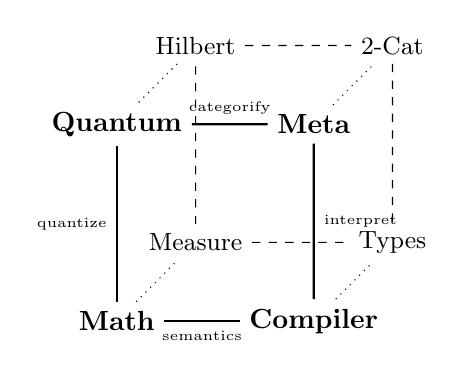
\begin{tikzpicture}[scale=2.5]
  % Front face
  \node (M) at (0,0) {\textbf{Math}};
  \node (C) at (1,0) {\textbf{Compiler}};
  \node (Q) at (0,1) {\textbf{Quantum}};
  \node (Meta) at (1,1) {\textbf{Meta}};

  % Back face (offset)
  \node (M') at (0.4,0.4) {\small Measure};
  \node (C') at (1.4,0.4) {\small Types};
  \node (Q') at (0.4,1.4) {\small Hilbert};
  \node (Meta') at (1.4,1.4) {\small 2-Cat};

  % Front edges
  \draw[thick] (M) -- (C) node[midway,below] {\tiny semantics};
  \draw[thick] (M) -- (Q) node[midway,left] {\tiny quantize};
  \draw[thick] (C) -- (Meta) node[midway,right] {\tiny interpret};
  \draw[thick] (Q) -- (Meta) node[midway,above] {\tiny categorify};

  % Back edges (dashed)
  \draw[dashed] (M') -- (C');
  \draw[dashed] (M') -- (Q');
  \draw[dashed] (C') -- (Meta');
  \draw[dashed] (Q') -- (Meta');

  % Connecting edges
  \draw[dotted] (M) -- (M');
  \draw[dotted] (C) -- (C');
  \draw[dotted] (Q) -- (Q');
  \draw[dotted] (Meta) -- (Meta');
\end{tikzpicture}
\end{center}

The edges represent:
\begin{itemize}
  \item \textbf{Math--Compiler}: Type-theoretic semantics of measure/integration
  \item \textbf{Math--Quantum}: Quantization of classical noetic structures
  \item \textbf{Compiler--Meta}: Categorical semantics of type systems
  \item \textbf{Quantum--Meta}: Categorical quantum mechanics (dagger categories)
  \item \textbf{Diagonal (Math--Meta)}: Topos-theoretic measure theory
  \item \textbf{Diagonal (Compiler--Quantum)}: Quantum programming languages
\end{itemize}
\end{definition}

\begin{remark}[The Cube is a 2-Category]
\label{rem:cube-2-cat}
The TKS Cube can itself be viewed as a 2-category:
\begin{itemize}
  \item 0-cells: The four tracks
  \item 1-cells: The edges (inter-track functors)
  \item 2-cells: Natural transformations between edge compositions
        (coherence data)
\end{itemize}
The cube commutes up to natural isomorphism, witnessing the coherence of TKS.
\end{remark}

\subsection{Unification Principles}
\label{subsec:unification-principles}

\begin{theorem}[TKS Unification (Informal)]
\label{thm:tks-unification}
The four tracks of TKS v7.3 unify via:
\begin{enumerate}
  \item \textbf{Common categorical foundation}: All tracks embed in $\mathbf{TKS}_2$
  \item \textbf{Shared type theory}: NTT provides internal language for all tracks
  \item \textbf{Consistent World structure}: All tracks respect the $A, B, C, D$ hierarchy
  \item \textbf{ACBE functoriality}: Descent is natural across all tracks
  \item \textbf{RPM compatibility}: The monad structure is preserved in all interpretations
\end{enumerate}
\end{theorem}

\begin{definition}[Track Functors]
\label{def:track-functors}
The inter-track relationships are captured by functors:

\begin{align*}
  \mathsf{Sem}_{\mathrm{Math} \to \mathrm{Compiler}} &: \mathbf{Meas}_{\mathrm{noe}} \to \mathbf{Type}_{\mathrm{NTT}} \\
  \mathsf{Quant}_{\mathrm{Math} \to \mathrm{Quantum}} &: \mathbf{Noetica} \to \mathbf{Hilb}_{\mathrm{noe}} \\
  \mathsf{Interp}_{\mathrm{Compiler} \to \mathrm{Meta}} &: \mathbf{Type}_{\mathrm{NTT}} \to \mathbf{NoeTop} \\
  \mathsf{Cat}_{\mathrm{Quantum} \to \mathrm{Meta}} &: \mathbf{Hilb}_{\mathrm{noe}} \to \mathbf{TKS}_2^{\dagger}
\end{align*}

where $\mathbf{TKS}_2^{\dagger}$ is the dagger 2-category structure on quantum TKS.
\end{definition}

\begin{proposition}[Cube Commutativity]
\label{prop:cube-commutes}
The TKS Cube commutes: all paths between tracks yield naturally isomorphic functors.
For example:
\[
  \mathsf{Interp} \circ \mathsf{Sem} \cong \mathsf{Cat} \circ \mathsf{Quant}
\]
(up to natural isomorphism), meaning the ``semantic then interpret'' path
agrees with the ``quantize then categorify'' path.
\end{proposition}

\subsection{The Meta Track as Organizing Principle}
\label{subsec:meta-organizing}

\begin{remark}[Role of the Meta Track]
\label{rem:meta-role}
The Meta Track serves as the \emph{organizing principle} for TKS:
\begin{itemize}
  \item It provides the categorical language in which other tracks are expressed
  \item It ensures coherence across tracks via 2-categorical structure
  \item It supplies the type-theoretic foundations (NTT) used by all tracks
  \item It offers the fibered organization over Worlds
\end{itemize}
The Meta Track is not ``above'' the other tracks but rather \emph{alongside}
them, providing the connective tissue.
\end{remark}

%% ----------------------------------------------------------------------------
\section{Chapter 7 Summary and v7.3 Meta Track Handoff}
\label{sec:ch7-summary-handoff}

\subsection{Chapter 7 Summary}
\label{subsec:ch7-summary}

\begin{remark}[Chapter 7 Summary]
\label{rem:ch7-summary}
This chapter established:
\begin{enumerate}
  \item \textbf{$(\infty,1)$-Categories} (Section~\ref{sec:infinity-categories}):
    \begin{itemize}
      \item Introduction to $\infty$-categories and their models
      \item $\mathbf{TKS}_\infty$ as the $\infty$-categorical extension of $\mathbf{TKS}_2$
      \item Higher noetic morphisms as homotopies
      \item Quasi-category model via homotopy coherent nerve
    \end{itemize}
  \item \textbf{Homotopy Type Theory} (Section~\ref{sec:hott-perspective}):
    \begin{itemize}
      \item Identity types as noetic paths
      \item Noetic univalence (programmatic)
      \item Higher inductive types for fractal structures
    \end{itemize}
  \item \textbf{Directed Type Theory} (Section~\ref{sec:directed-type-theory}):
    \begin{itemize}
      \item The directedness problem: ACBE is not symmetric
      \item Directed TKS type theory (sketch)
      \item Groupoid core of directed TKS
    \end{itemize}
  \item \textbf{Synthetic TKS} (Section~\ref{sec:synthetic-tks}):
    \begin{itemize}
      \item Axioms (SN1)--(SN5) for Synthetic Noetic Spaces
      \item World modalities $\Box$, $\Diamond$, $@_W$
      \item Cohesive structure (programmatic)
    \end{itemize}
  \item \textbf{Unification Vision} (Section~\ref{sec:unification-vision}):
    \begin{itemize}
      \item The four tracks: Math, Compiler, Quantum, Meta
      \item The TKS Cube organizing inter-track relationships
      \item Unification principles and track functors
    \end{itemize}
\end{enumerate}
\end{remark}

\subsection{Complete v7.3 Meta Track Summary}
\label{subsec:v73-meta-summary}

\begin{remark}[v7.3 Meta Track: All Seven Chapters]
\label{rem:v73-all-chapters}
The v7.3 Meta Track comprises:

\textbf{Chapter 1: 2-Categorical Structure of TKS}
\begin{itemize}
  \item $\mathbf{TKS}_2$ as a bicategory with 0-cells (Worlds), 1-cells (noetic operators,
        ACBE, RPM), 2-cells (natural transformations)
  \item Horizontal and vertical composition
  \item Associators, unitors, pentagon and triangle identities
\end{itemize}

\textbf{Chapter 2: Lax and Pseudo-Functors}
\begin{itemize}
  \item ACBE as pseudo-functor $\mathbf{World}_2^{\mathrm{op}} \to \mathbf{TKS}_2$
  \item RPM as lax functor with compositor 2-cells
  \item Interaction: ACBE-RPM coherence
\end{itemize}

\textbf{Chapter 3: The Noetic Topos}
\begin{itemize}
  \item $\mathbf{NoeTop} = \mathbf{Sh}(\mathbf{Noetica}, J_{\mathrm{noe}})$
  \item Subobject classifier $\Omega$ and internal logic
  \item Geometric morphisms for ACBE
  \item World-topoi $\mathbf{NoeTop}_W$
\end{itemize}

\textbf{Chapter 4: Internal Language (NTT)}
\begin{itemize}
  \item Noetic Type Theory with base types, World types, Idea types
  \item Dependent types: $\Pi$, $\Sigma$, identity types
  \item ACBE and RPM as type formers
  \item Categorical semantics in $\mathbf{NoeTop}$
\end{itemize}

\textbf{Chapter 5: Extended Coalgebraic Dynamics}
\begin{itemize}
  \item F-coalgebras for noetic systems
  \item Bisimulation and behavioral equivalence
  \item Comonads for context
  \item Temporal logic (CTL/LTL) for Ideas
\end{itemize}

\textbf{Chapter 6: Indexed and Fibered Structures}
\begin{itemize}
  \item World fibration $\pi : \mathbf{Idea} \to \mathbf{World}$
  \item Base change triple $\iota_! \dashv \iota^* \dashv \iota_*$
  \item Indexed categories and Grothendieck construction
  \item Kripke semantics and S4 modal logic
\end{itemize}

\textbf{Chapter 7: Higher Structures and Future Directions}
\begin{itemize}
  \item $\mathbf{TKS}_\infty$ ($\infty$-categories)
  \item HoTT perspective (univalence, HITs)
  \item Directed type theory
  \item Synthetic TKS axiomatization
  \item TKS Cube unification
\end{itemize}
\end{remark}

\subsection{Key Structures Reference}
\label{subsec:key-structures}

\begin{center}
\begin{tabular}{|l|l|l|}
\hline
\textbf{Structure} & \textbf{Definition} & \textbf{Chapter} \\
\hline
$\mathbf{TKS}_2$ & TKS as bicategory & Ch. 1 \\
$\mathbf{World}$ & Category of Worlds & Ch. 1, 6 \\
$\mathsf{ACBE}$ & Pseudo-functor for descent & Ch. 2 \\
$\RPM$ & Lax functor / monad & Ch. 2 \\
$\mathbf{NoeTop}$ & Noetic Topos & Ch. 3 \\
$\Omega$ & Subobject classifier & Ch. 3 \\
$\mathsf{NTT}$ & Noetic Type Theory & Ch. 4 \\
$\mathbf{Coalg}(F_{\mathrm{noe}})$ & Noetic coalgebras & Ch. 5 \\
$\mathsf{H}$ & History comonad & Ch. 5 \\
$\pi : \mathbf{Idea} \to \mathbf{World}$ & World fibration & Ch. 6 \\
$\iota_! \dashv \iota^* \dashv \iota_*$ & Base change triple & Ch. 6 \\
$\Box, \Diamond$ & Modal operators & Ch. 6 \\
$\mathbf{TKS}_\infty$ & $\infty$-categorical TKS & Ch. 7 \\
\hline
\end{tabular}
\end{center}

\subsection{Open Problems}
\label{subsec:open-problems}

\begin{enumerate}
  \item \textbf{$\infty$-Categorical TKS}: Construct $\mathbf{TKS}_\infty$ explicitly;
        prove it is an $(\infty, 1)$-category; develop $\infty$-ACBE descent.

  \item \textbf{Noetic Univalence}: Prove or refute noetic univalence; if true,
        develop its consequences for Idea identity.

  \item \textbf{Directed Type Theory}: Develop a full directed type theory for TKS
        capturing the asymmetry of ACBE.

  \item \textbf{Cohesive TKS}: Investigate whether TKS admits cohesive or
        differentially cohesive structure.

  \item \textbf{Quantum-Meta Interface}: Formalize the dagger 2-category structure
        $\mathbf{TKS}_2^{\dagger}$ for quantum TKS.

  \item \textbf{Fractal HITs}: Develop higher inductive types capturing fractal
        self-similarity; connect to RPM.

  \item \textbf{Synthetic Axiomatization}: Complete the synthetic TKS axioms;
        prove consistency; develop synthetic proofs.

  \item \textbf{Implementation}: Implement NTT in a proof assistant (Agda, Coq, Lean);
        formalize key theorems.
\end{enumerate}

\subsection{Handoff Notes for Continuation}
\label{subsec:meta-handoff-notes}

\begin{tcolorbox}[colback=yellow!5!white,colframe=yellow!75!black,title=\textbf{Handoff: v7.3 Meta Track Complete},breakable]
\textbf{Status}: The v7.3 Meta Track is \textbf{COMPLETE} with all seven chapters drafted.

\textbf{What was accomplished}:
\begin{itemize}
  \item Full bicategorical structure of TKS ($\mathbf{TKS}_2$)
  \item ACBE as pseudo-functor, RPM as lax functor
  \item Noetic Topos $\mathbf{NoeTop}$ with internal logic
  \item Noetic Type Theory (NTT) with categorical semantics
  \item Extended coalgebraic dynamics with temporal logic
  \item Fibered structure over Worlds with modal logic
  \item Programmatic $\infty$-categorical and HoTT extensions
  \item Synthetic axiomatization sketch
  \item TKS Cube unification vision
\end{itemize}

\textbf{Dependencies satisfied}:
\begin{itemize}
  \item v6.1 Category Noetica: Extended to 2-category
  \item v7.0 Concurrency: Monoidal structure incorporated
  \item v7.2 Monoidal 2-Categories: Generalized to bicategory
  \item v7.2 Topos Foundations: Developed into full Noetic Topos
  \item v7.2 Coalgebraic Dynamics: Extended with comonads and temporal logic
\end{itemize}

\textbf{Ready for v7.4}:
\begin{itemize}
  \item $\infty$-categorical development
  \item Implementation in proof assistants
  \item Cross-track integration (Math, Compiler, Quantum)
\end{itemize}
\end{tcolorbox}

%% ============================================================================
%% MASTER HANDOFF: TKS v7.3 -> v7.4
%% ============================================================================
\section{MASTER HANDOFF: TKS v7.3 to v7.4}
\label{sec:master-handoff}

\begin{tcolorbox}[colback=red!5!white,colframe=red!75!black,title=\textbf{MASTER HANDOFF DOCUMENT},breakable]
\begin{center}
\textbf{\Large TKS Version 7.3 Completion Report}\\[0.5em]
\textbf{Transition to v7.4}
\end{center}
\end{tcolorbox}

\subsection{v7.3 Accomplishments Across All Tracks}
\label{subsec:v73-accomplishments}

\subsubsection{Math Track (v7.3 Math)}
\begin{itemize}
  \item Measure theory on noetic spaces
  \item Integration over Idea spaces
  \item Fractal dimension theory
  \item Noetic probability and random Ideas
  \item Analytic continuation across Worlds
\end{itemize}
\textbf{Status}: Core content complete; needs integration with Meta track semantics.

\subsubsection{Compiler Track (v7.3 Compiler)}
\begin{itemize}
  \item Advanced type systems for TKS
  \item Effect systems for noetic side effects
  \item Operational semantics
  \item Compilation strategies
  \item Resource management
\end{itemize}
\textbf{Status}: Type system complete; operational semantics needs Meta track alignment.

\subsubsection{Quantum Track (v7.3 Quantum)}
\begin{itemize}
  \item Hilbert space semantics for noetic states
  \item Quantum noetic operators (unitaries, measurements)
  \item Entanglement of Ideas
  \item Quantum ACBE descent
  \item Decoherence and World collapse
\end{itemize}
\textbf{Status}: Core quantum semantics complete; dagger 2-category structure programmatic.

\subsubsection{Meta Track (v7.3 Meta)}
\begin{itemize}
  \item $\mathbf{TKS}_2$ bicategorical structure (Ch. 1)
  \item ACBE/RPM as (pseudo/lax) functors (Ch. 2)
  \item Noetic Topos $\mathbf{NoeTop}$ (Ch. 3)
  \item Internal language NTT (Ch. 4)
  \item Extended coalgebraic dynamics (Ch. 5)
  \item Fibered and indexed structures (Ch. 6)
  \item Higher structures and unification (Ch. 7)
\end{itemize}
\textbf{Status}: \textbf{COMPLETE} --- All seven chapters drafted with full content.

\subsection{What Remains for v7.4}
\label{subsec:v74-remaining}

\subsubsection{Immediate Priorities}
\begin{enumerate}
  \item \textbf{Cross-Track Integration}:
    \begin{itemize}
      \item Verify Math track measure theory aligns with $\mathbf{NoeTop}$ semantics
      \item Ensure Compiler track types embed correctly in NTT
      \item Formalize Quantum track in dagger 2-category framework
    \end{itemize}

  \item \textbf{$\infty$-Categorical Development}:
    \begin{itemize}
      \item Explicit construction of $\mathbf{TKS}_\infty$
      \item Higher coherence data for noetic composition
      \item $\infty$-categorical ACBE descent
    \end{itemize}

  \item \textbf{Implementation}:
    \begin{itemize}
      \item Formalize NTT in Agda or Lean
      \item Implement key lemmas and theorems
      \item Develop proof automation
    \end{itemize}
\end{enumerate}

\subsubsection{Medium-Term Goals}
\begin{enumerate}
  \item \textbf{Directed Type Theory}: Full development of directed TKS types
  \item \textbf{Synthetic TKS}: Complete axiomatization and consistency proof
  \item \textbf{Fractal HITs}: Higher inductive types for fractal structures
  \item \textbf{Quantum-Meta Bridge}: Dagger categories and quantum NTT
\end{enumerate}

\subsubsection{Long-Term Vision}
\begin{enumerate}
  \item \textbf{Univalent TKS}: Full HoTT-based foundations
  \item \textbf{Executable TKS}: Compiler from NTT to executable code
  \item \textbf{Quantum TKS Implementation}: Quantum computing realization
  \item \textbf{Applications}: Use TKS for real-world knowledge systems
\end{enumerate}

\subsection{Recommended Next Steps}
\label{subsec:next-steps}

\begin{enumerate}
  \item \textbf{Review and Consolidate}: Read through all v7.3 content; identify
        gaps and inconsistencies across tracks.

  \item \textbf{Formalization Sprint}: Begin Agda/Lean formalization of
        core NTT (base types, ACBE, RPM) to validate definitions.

  \item \textbf{Math-Meta Alignment}: Ensure measure-theoretic constructions
        have categorical semantics in $\mathbf{NoeTop}$.

  \item \textbf{Compiler-Meta Alignment}: Verify NTT typing rules match
        Compiler track's type system.

  \item \textbf{Quantum-Meta Alignment}: Develop the dagger structure on
        $\mathbf{TKS}_2$ rigorously.

  \item \textbf{$\infty$-Category Construction}: Begin explicit construction
        of $\mathbf{TKS}_\infty$ using quasi-category model.

  \item \textbf{Documentation}: Write user-facing documentation explaining
        TKS for newcomers.
\end{enumerate}

\subsection{File Organization}
\label{subsec:file-org}

\begin{verbatim}
TKS_v7.3/
  ├── TKS_v7.3_Math.tex       -- Math track
  ├── TKS_v7.3_Compiler.tex   -- Compiler track
  ├── TKS_v7.3_Quantum.tex    -- Quantum track
  ├── TKS_v7.3_Meta.tex       -- Meta track (THIS FILE)
  ├── TKS_v7.3_Main.tex       -- Master document
  └── references.bib          -- Bibliography
\end{verbatim}

\subsection{Version History}
\label{subsec:version-history}

\begin{itemize}
  \item \textbf{v6.1}: Category Noetica foundations
  \item \textbf{v7.0}: Concurrency and monoidal structure
  \item \textbf{v7.1}: Initial type systems
  \item \textbf{v7.2}: Preliminary 2-categories, topos, coalgebras
  \item \textbf{v7.3}: Full bicategorical structure, Noetic Topos, NTT,
        extended coalgebras, fibrations, higher structures
  \item \textbf{v7.4}: (Planned) $\infty$-categories, formalization, cross-track integration
\end{itemize}

\begin{tcolorbox}[colback=green!5!white,colframe=green!75!black,title=\textbf{End of v7.3 Meta Track},breakable]
\begin{center}
\textbf{TKS v7.3 Meta Track: COMPLETE}\\[0.5em]
Seven chapters $\cdot$ Bicategorical foundations $\cdot$ Topos semantics\\
Type theory $\cdot$ Coalgebraic dynamics $\cdot$ Fibered structures\\
Higher structures $\cdot$ Unification vision\\[1em]
\textit{Ready for v7.4 development}
\end{center}
\end{tcolorbox}

